\documentclass[11pt,aspectratio=169]{beamer}

% --- Tema og fonte ---
\usetheme{Madrid}
\usefonttheme{serif}
% --- Farver ---
\definecolor{myteal}{RGB}{14,71,57}
\setbeamercolor{title}{fg=white}
\setbeamercolor{frametitle}{fg=white,bg=myteal}
\setbeamercolor{block title}{fg=white,bg=myteal}
\setbeamercolor{block body}{bg=myteal!10}
\setbeamercolor{normal text}{fg=myteal}
\setbeamercolor{background canvas}{bg=white}
\setbeamercolor{structure}{fg=myteal}
\setbeamercolor{palette primary}{fg=white,bg=myteal}
\setbeamercolor{palette secondary}{fg=white,bg=myteal!80}
\setbeamercolor{palette tertiary}{fg=white,bg=myteal!60}
\setbeamercolor{author in head/foot}{fg=white,bg=myteal}
\setbeamercolor{title in head/foot}{fg=white,bg=myteal!80}
\setbeamercolor{date in head/foot}{fg=white,bg=myteal!60}
\setbeamercolor{titlelike}{fg=myteal}
\setbeamercolor{section in toc}{fg=myteal}
\setbeamercolor{item}{fg=myteal}
% --- Sprog og encoding ---
\usepackage[utf8]{inputenc}
\usepackage[danish]{babel}
\usepackage[T1]{fontenc}
\usepackage{lmodern}
% --- Matematik ---
\usepackage{amsmath,amsfonts,amssymb}
% --- Grafik og layout ---
\usepackage{graphicx}
\usepackage{ragged2e}
\usepackage{booktabs}
\usepackage{arydshln}
\usepackage[most]{tcolorbox}
% --- Ikoner og figurer ---
\usepackage{fontawesome5}
\usepackage{tikz}
\usetikzlibrary{positioning,arrows.meta,shapes.geometric,calc}
\usepackage{circuitikz}
% --- Positionering ---
\usepackage[absolute,overlay]{textpos}
% --- CSV ---
\usepackage{csvsimple}
% --- Kildehenvisning nederst på slides ---
\setbeamercolor{framesource}{fg=gray,bg=white}
\setbeamerfont{framesource}{size=\scriptsize}
\newcommand{\framesource}[1]{%
  \begin{textblock*}{12cm}(0.5cm,8.6cm)
    \raggedleft
    \beamercolorbox[wd=\textwidth,rightskip=0.5cm]{framesource}{#1}
  \end{textblock*}
}
% --- Automatisk billedattribution ---
\csvreader[
  head to column names,
  no head
]{Billeder/billedkilder.csv}{}{}
\newcommand{\billedkilde}[1]{%
  \csvreader[
    head to column names,
    full filter=\ifcsvstrcmp{\filnavn}{#1}{\csvfilteraccept}{\csvfilterreject},
    no head
  ]{Billeder/billedkilder.csv}{}%
  {%
    \tiny\forfatter\ / Wikimedia Commons (\licens)%
  }%
}
% --- Boksstile til jagttid-sliden ---
\tcbset{
  gruppe/.style={
    enhanced,
    colback=white,
    colframe=myteal,
    coltitle=myteal,
    boxrule=0.8pt,
    dashed,
    sharp corners,
    fonttitle=\bfseries\large,
    attach boxed title to top left={yshift=-2mm,xshift=3mm},
    boxed title style={colback=white,colframe=white,boxrule=0pt,sharp corners},
    top=1mm,left=1mm,right=1mm,bottom=1mm
  },
  felt/.style={
    enhanced,
    colback=white,
    colframe=myteal,
    boxrule=0.6pt,
    sharp corners,
    halign=center,
    valign=center,
    width=\linewidth,
    height=1.55cm,
    fit,
    fit algorithm=fontsize,
    fit basedim=7pt,
    boxsep=0.3mm,
    left=0.5mm, right=0.5mm, top=0.3mm, bottom=0.3mm
  },
  feltfri/.style={
    enhanced,
    colback=white,
    colframe=myteal,
    boxrule=0.6pt,
    sharp corners,
    halign=center,
    valign=center,
    width=\linewidth,
    boxsep=0.3mm,
    left=0.5mm, right=0.5mm, top=0.3mm, bottom=0.3mm,
    fontupper=\scriptsize
  }
}
% --- Matematiske operatorer ---
\DeclareMathOperator{\sen}{sen}
\DeclareMathOperator{\tg}{tg}
% --- Beamer-indstillinger ---
\setbeamertemplate{caption}[numbered]
\setbeamertemplate{navigation symbols}{}
% --- Forfatter ---
\author[Østerbro Jagttegn]{Østerbro Jagttegn \\ \textbf{Aleksander Sønder}}
% --- Hyperref (altid sidst) ---
\usepackage{hyperref}
\hypersetup{
  colorlinks=true,
  linkcolor=myteal,
  urlcolor=myteal,
  citecolor=myteal
}

\title[Modul 2]{Modul 2 \\
Obligatorisk Jagttegnskursus \\ @ Microsoft 17:30-21:00}
\date{\today}

\begin{document}

% Titelside
\begin{frame}
  \titlepage
\end{frame}

% Indholdsfortegnelse (valgfri)
\begin{frame}{Program}
  \tableofcontents
\end{frame}


\section{Våbenbekendtgørelsen}

\begin{frame}
\vspace{3em}
\begin{center}
{\LARGE \textbf{Bekendtgørelse om våben og ammunition mv.}}
\vspace{2em}
\par
% Våbenbekendtgørelsen
{\normalsize \href{https://www.retsinformation.dk/eli/lta/2021/2531}{BEK nr 2531 af 20/12/2021}}
\vspace{1em}
\par

\end{center}
\end{frame}

\begin{frame}{Adgang til Våben: Jagttegn og Tilladelser}

\vspace{1em}

\begin{columns}[c] % c = center vertically

\column{0.05\textwidth} % Venstre margin

\column{0.7\textwidth} % Midten: Bullets

\small

\raggedright

\begin{itemize}

\itemsep0.6em % Justér afstand mellem bullets

\item Et jagttegn udstedes kun med \textbf{samtykke fra Politiet} (vurdering af vandel/egnethed, jf. § 6).

\item Du skal være fyldt \textbf{18 år} for selv at kunne \structure{erhverve} og \structure{besidde} skydevåben.

\item Våben må kun håndteres af personer, der kan fremvise \textbf{gyldigt jagttegn} eller \structure{våbentilladelse} (§ 20).

\item Du må bruge haglgevær under \structure{jagtprøven} og til instruktion, da kursuslærere må overlade våben til dig (§ 21).

\item \textbf{Ungjægerordningen}: Er du under 18 år, skal du jage \textbf{i følge med} en myndig jæger (over 18 år).

\end{itemize}

\column{0.25\textwidth} % Højre: Ikon

\centering

\vspace{0pt}

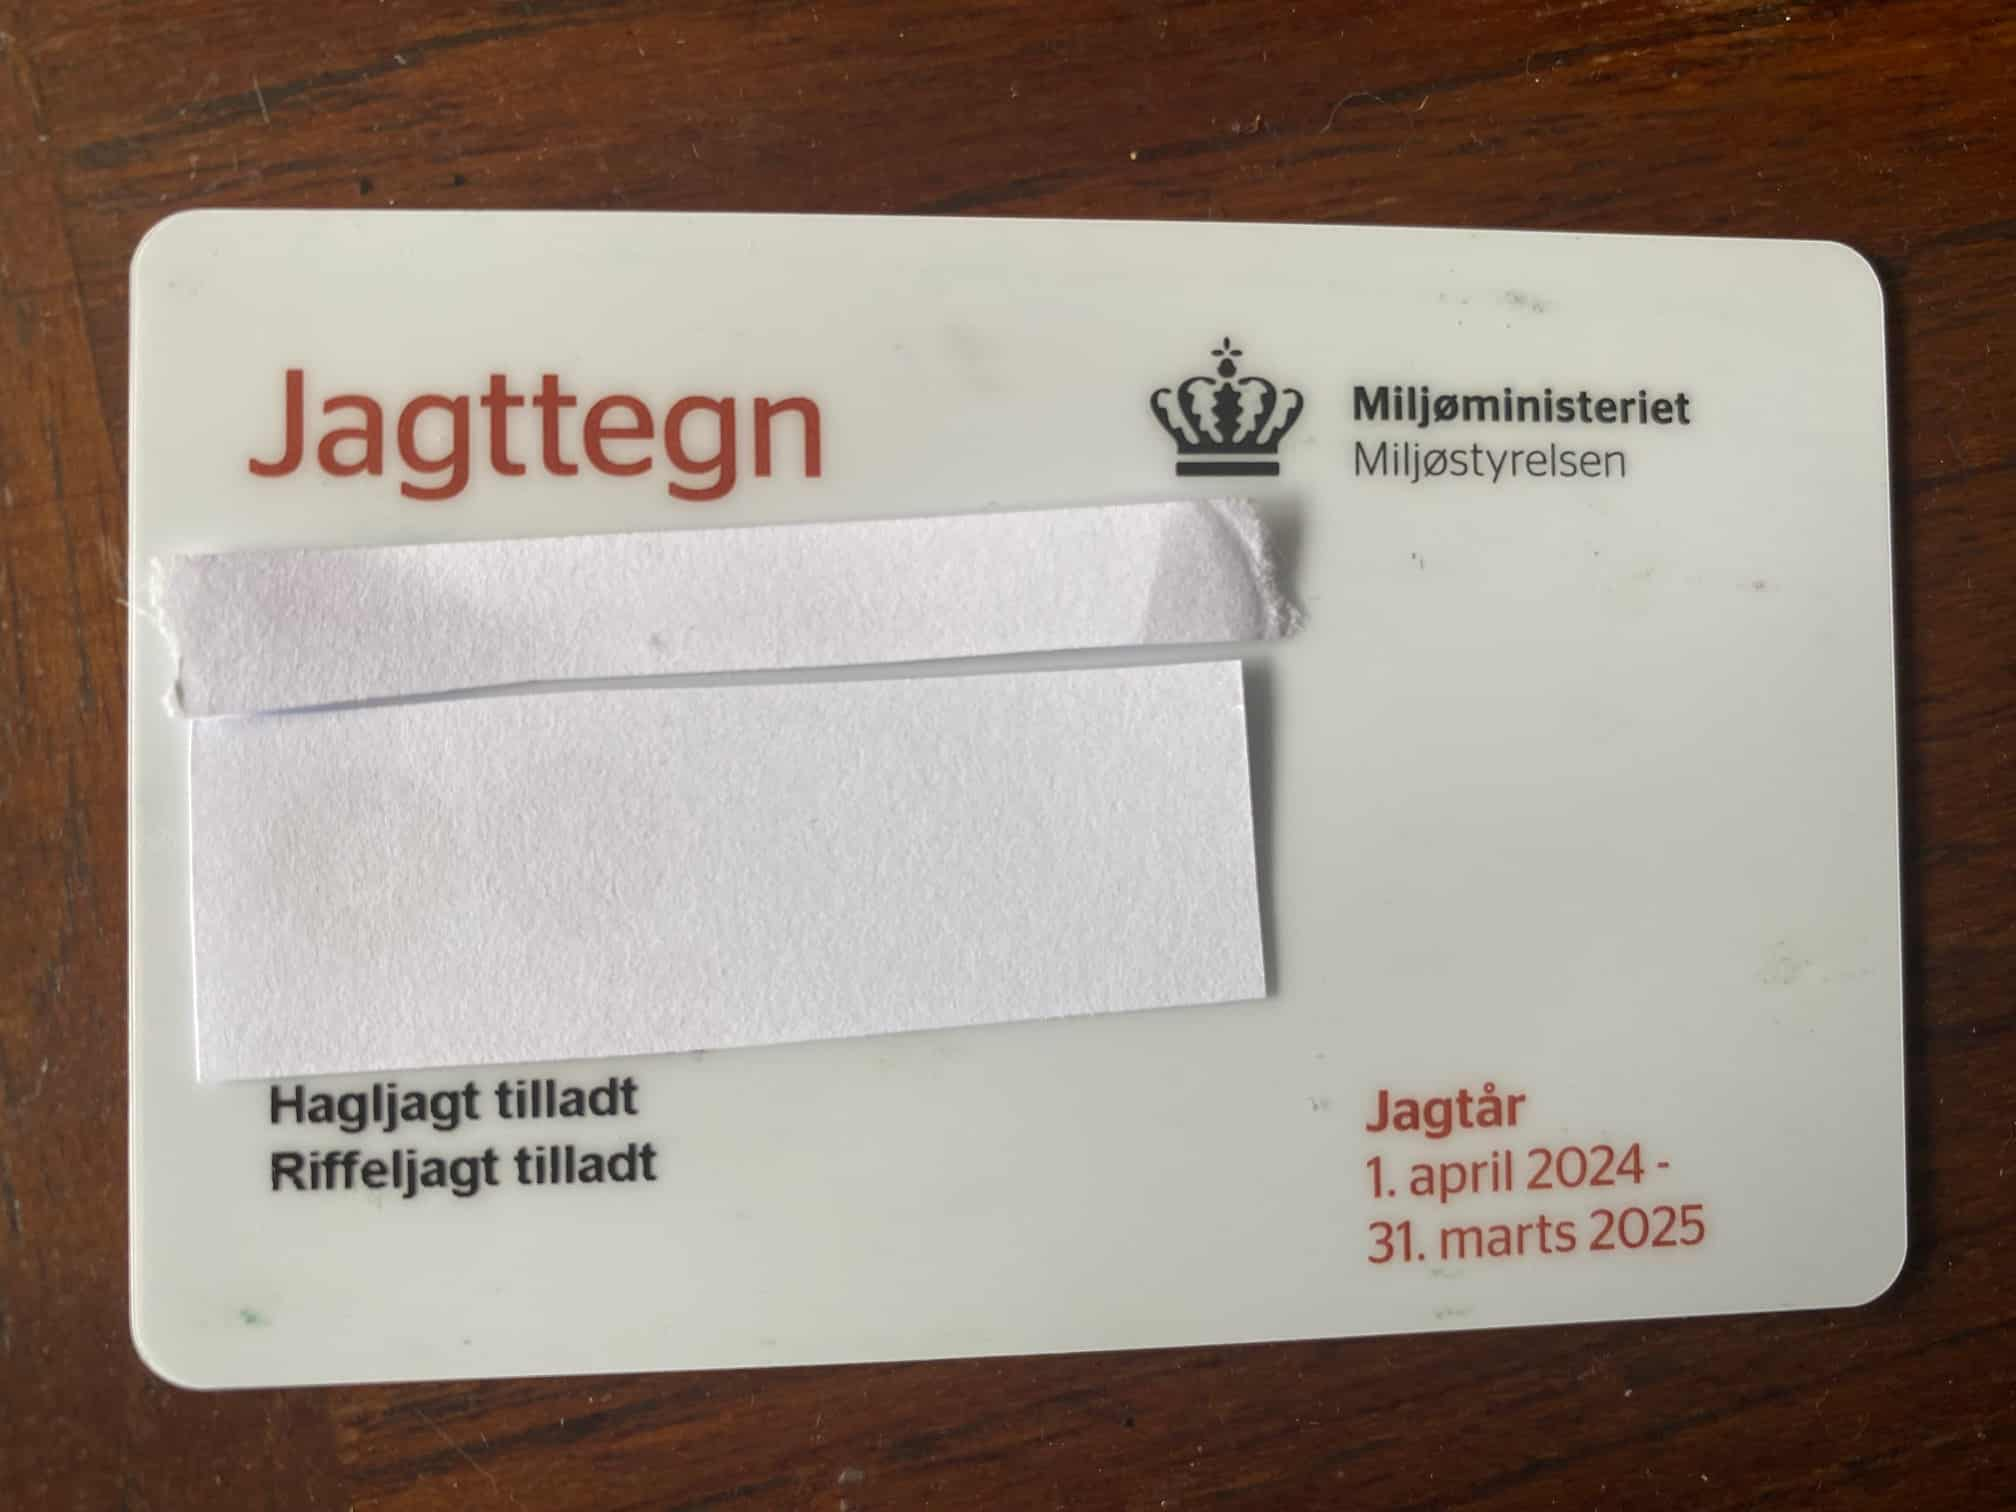
\includegraphics[width=0.9\linewidth]{Billeder/Redskaber/jagttegn_billede.jpg} % Antager et ikon, der passer til 'Tilladelse' (evt. et jagttegn)

\end{columns}

\end{frame}
\begin{frame}{Opbevaring af våben og ammunition § 24}

\vspace{1em}

\begin{columns}[c] % c = center vertically

\column{0.05\textwidth} % Venstre margin (kan fjernes eller justeres)



\column{0.7\textwidth} % Midten: Bullets

\small

\raggedright



\begin{itemize}

\itemsep0.6em % Justér afstand mellem bullets

\item Våben og ammunition skal opbevares forsvarligt og \textbf{utilgængeligt} for uvedkommende.

\item Skabe under \textbf{1.000 kg} skal være fastboltet til gulv/væg.

\item Nøgler til skabet skal opbevares separat og utilgængeligt.

\item Der sondres mellem to typer af våbenskabe, som styres af antallet af våben, der skal opbevares.

\item Max 25 regulære våben, hvor max 10 våben må være særligt farlige våben \textbf{kræver} (min. EN 1143-1 \textbf{Grade 0}).

\item Flere end 25 regulære våben og/eller 10 særligt farlige våben \textbf{kræver} (min. EN 1143-1 \textbf{Grade 1}).

\item Ammunition må opbevares ved siden af, men ikke i våbnet.

\end{itemize}



\column{0.25\textwidth} % Højre: Ikon (størrelsen tilpasses her)

\centering

\vspace{0pt} % hjælper med vertikal centring i nogle temaer

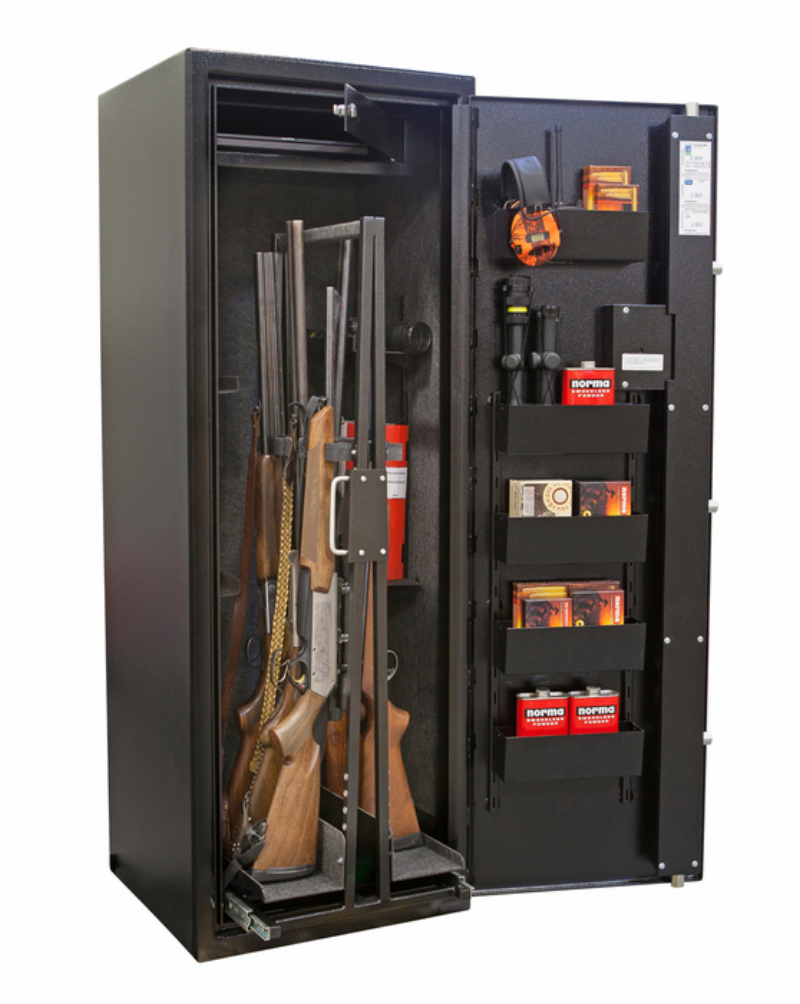
\includegraphics[width=0.8\linewidth]{Billeder/Redskaber/vaabenskab.png}



\end{columns}

\end{frame}
\begin{frame}{Særligt farlige våben og sikringskrav}

\begin{itemize}
    \item \textbf{Særligt farlige våben} (defineret i bekendtgørelsen):
    \begin{itemize}
        \item Pistoler (inkl. enkeltskud, halvautomatiske, revolvere – undtagen forladevåben)
        \item Fuld- og halvautomatiske våben (halvautomatisk haglgevær)
        \item Glatløbede haglgeværer med pibelængde under 55 cm
    \end{itemize}
    \vspace{1em}
    \item \textbf{Vigtigt at huske}:
    \begin{itemize}
        \item Det samlede antal våben på adressen afgør sikringskravet – også selvom våbnene opbevares i flere skabe
        \item Sikringsniveauet er strengere for særligt farlige våben, da de anses for en større risiko end et højere antal almindelige våben
    \end{itemize}
\end{itemize}

\end{frame}
\begin{frame}{Overdragelse og Overladelse af Våben (§ 20)}

\vspace{1em}

\begin{columns}[c] % c = center vertically

\column{0.05\textwidth} % Venstre margin

\column{0.7\textwidth} % Midten: Bullets

\small

\raggedright

\begin{itemize}

\itemsep0.3em % Justér afstand mellem bullets

\item \textbf{Hovedregel:} Våben må kun overdrages eller overlades til personer, der kan fremvise \structure{fornøden våbentilladelse}.

\item \textbf{Forskel riffel og haglvåben:} Haglvåben kan overlades til en anden person med jagttegn. Riffel må kun overdrages til person med våbentilladelse til pågældende våben.

\item \textbf{Identifikation:} Den, der modtager våbnet, skal fremvise \structure{original billedlegitimation} for at bevise, at tilladelsen tilhører vedkommende.

\item \textbf{Udlåners ansvar:} Den, der låner våbnet ud, har pligt til at kontrollere \structure{både tilladelse og legitimation}.

\item \textbf{Ungjægere:} Glatløbede haglgeværer må overlades til kursister/aspiranter af \textbf{godkendte lærere/prøvesagkyndige} i forbindelse med instruktion og prøve (§ 21).

\end{itemize}

\column{0.25\textwidth} % Højre: Ikon

\centering

\vspace{0pt}

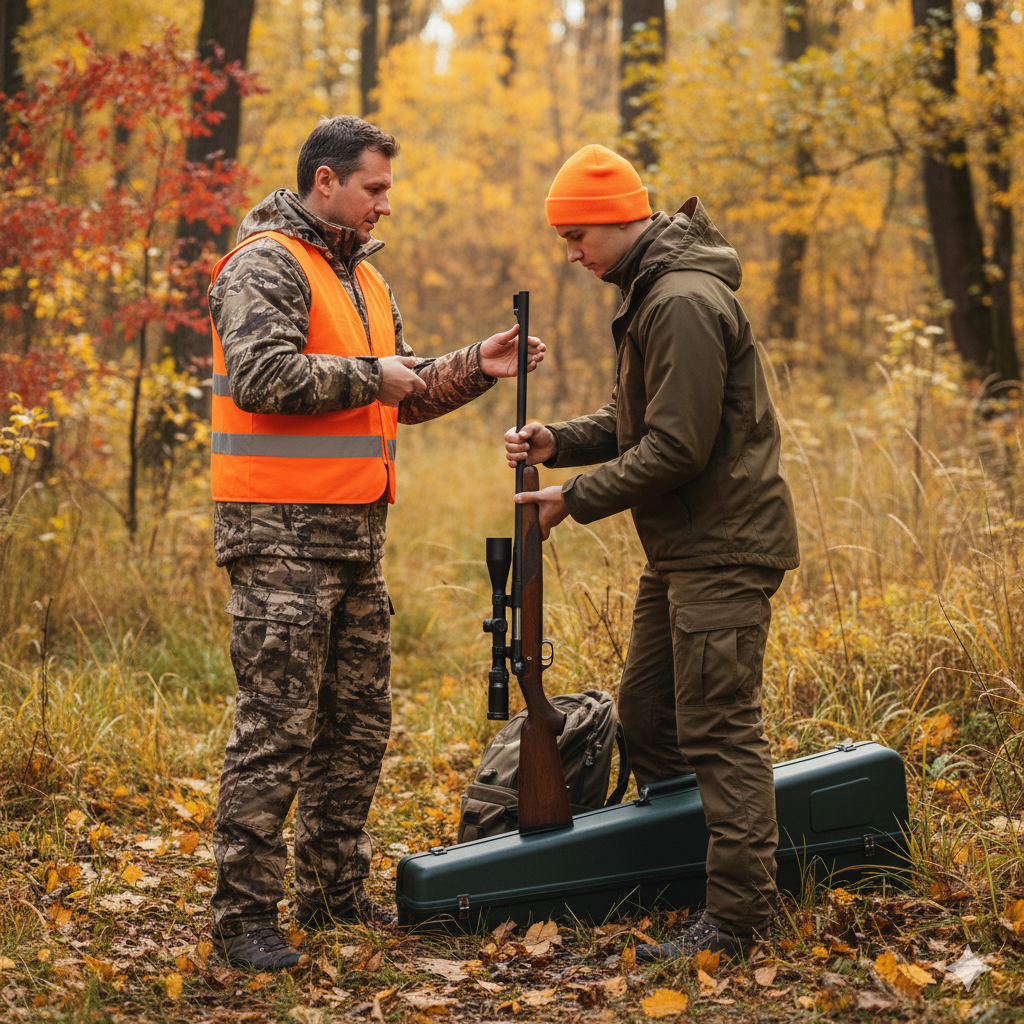
\includegraphics[width=0.9\linewidth]{Billeder/Redskaber/overdragelse.png} % Forslag til et ikon, der symboliserer overladelse/aftale

\end{columns}

\end{frame}
\begin{frame}{Transport af Skydevåben (§ 11)}

\vspace{1em}

\begin{columns}[c] % c = center vertically

\column{0.05\textwidth} % Venstre margin

\column{0.7\textwidth} % Midten: Bullets

\small

\raggedright

\begin{itemize}

\itemsep0.6em % Justér afstand mellem bullets

\item \textbf{Formål:} Transport må kun ske i forbindelse med anerkendelsesværdige formål (f.eks. til/fra \structure{opbevaring, anvendelsessted, køb/salg eller reparation}).

\item \textbf{Forsvarlighed:} Våben skal transporteres \textbf{forsvarligt} (f.eks. under konstant tilsyn eller tildækket i aflåst transportmiddel).

\item \textbf{Indpakning:} Skydevåben skal være \structure{indpakket i lukket etui eller lignende} (f.eks. våbenkuffert).

\item \textbf{Ammunition:} Skydevåben må \textbf{IKKE indeholde ammunition} under transport uden for anvendelsesområdet (jagt/skydebane).

\item \textbf{Bæring:} Våben må \textbf{IKKE} transporteres i side- eller skulderhylstre på kroppen.

\end{itemize}

\column{0.25\textwidth} % Højre: Ikon

\centering

\vspace{0pt}

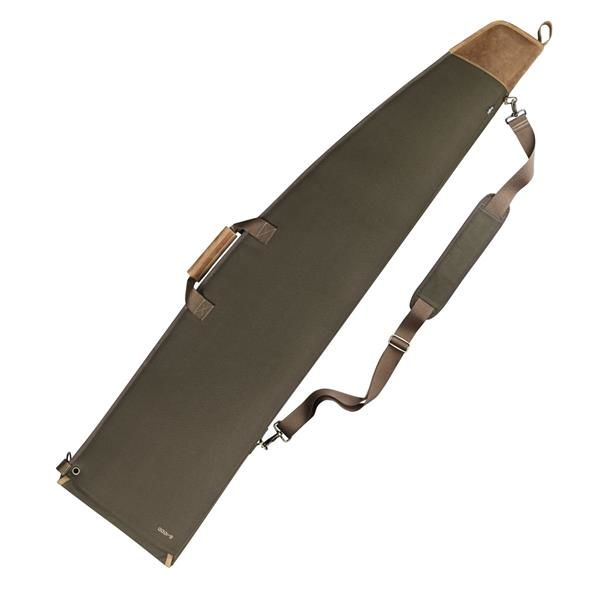
\includegraphics[width=0.9\linewidth]{Billeder/Redskaber/futeral.jpg} % Forslag til et ikon, der symboliserer transport/bil

\end{columns}

\end{frame}
\section{Cirkulære om våben og ammunition m.v.}

\begin{frame}
  \vspace{3em}
  \begin{center}
    {\LARGE \textbf{Cirkulære om våben og ammunition m.v.}} \\
    \vspace{1em}
    CIR1H nr 10066 af 29/10/2025, § 16
  \end{center}
\end{frame}

\begin{frame}{\S\ 16, Personer under 18 år}
\begin{itemize}
    \item Tilladelse kan gives til personer under 18 år, hvis de:
    \begin{itemize}
        \item er medlem af skytte- eller jagtforening og fyldt 16 år, eller
        \item har jagttegn
    \end{itemize}
    \item Personer fyldt 16 år kan desuden få tilladelse til luft-/fjedervåben ($\leq$ 4,5 mm)
    \item Tilladelse til foreningsmedlemmer gælder kun våben, der anvendes i foreningen
    \item Tilladelse kræver skriftligt samtykke fra forældremyndighedsindehavere, som også påtager sig opbevaringsansvar
    \item Politiet skal sikre, at forældre er bekendt med rettigheder/pligter og opfylder opbevaringskrav (\S\ 48 i våbenbekendtgørelsen)
\end{itemize}
\end{frame}
\section{Årefodede fugle}

\begin{frame}
  \vspace{3em}
  \begin{center}
    {\LARGE \textbf{Årefodede fugle}}
    \vspace{2em}
    \\ Artsbestemmelse og vildtbiologi
\par
{\normalsize }
\vspace{1em}
\par
  \end{center}
\end{frame}

\begin{frame}{%
\begin{minipage}[t]{0.85\textwidth}
Skarv (mellemskarv og storskarv)
\end{minipage}%
\hfill
\begin{minipage}[t]{0.1\textwidth}
\raggedleft

\includegraphics[width=0.5cm, height=0.5cm, keepaspectratio]{Billeder/Ikoner/star.png}%
\hspace{0.2em}%

\includegraphics[width=0.5cm, height=0.5cm, keepaspectratio]{Billeder/Ikoner/star.png}
\end{minipage}%
}
\vspace{0.25em}
\begin{columns}[T]
% --- Venstre kolonne: Tekst ---
\column{0.55\textwidth}
\setlength{\parskip}{0.5em}
\small
\RaggedRight\textbf{\textit{Phalacrocorax carbo}} – Sort fugl også kaldet ålekrage \par % Rettet til Troldand's latinske navn og beskrivelse

\textbf{Udseende:} \\
\quad – Slank sort med kraftig gult næb der er tydeligt nedadbøjet i spidsen \par

\textbf{Levesteder:} \\
\quad – Kyster, fjorde, søer og større vandløb

\textbf{Føde:} \\
\quad – Fisk \par

\textbf{Udbredelse:} \\
\quad – Hele Danmark \par

\textbf{Træk/standfugl} \\
\quad – Mellemskarv yngler, storskarv er trækfugl \par

% --- Højre kolonne: Kun ét billede (Hannen) ---
\column{0.40\textwidth}
\centering
\fbox{%
\begin{minipage}{\linewidth}
\centering
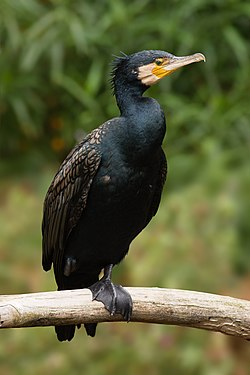
\includegraphics[width=0.8\linewidth, height=6.5cm, keepaspectratio]{Billeder/Dyr/Fugle/Skarver/skarv.jpg}%
\end{minipage}
}%
\end{columns}
\end{frame}
\section{Storkefugle}

\begin{frame}
  \vspace{3em}
  \begin{center}
    {\LARGE \textbf{Storkefugle}}
    \vspace{2em}
    \\ Artsbestemmelse og vildtbiologi
\par
{\normalsize }
\vspace{1em}
\par
  \end{center}
\end{frame}

\begin{frame}{%
\begin{minipage}[t]{0.85\textwidth}
Fiskehejre
\end{minipage}%
\hfill
\begin{minipage}[t]{0.1\textwidth}
\raggedleft

\includegraphics[width=0.55cm, height=0.55cm, keepaspectratio]{Billeder/Ikoner/star.png}%
\end{minipage}%
}
\vspace{0.25em}
\begin{columns}[T]
% --- Venstre kolonne: Tekst ---
\column{0.55\textwidth}
\setlength{\parskip}{0.5em}
\small
\RaggedRight\textbf{\textit{Ardea cinerea}} – Særegen storkelignende slank fugl der jager langs kyster, søer, vandløb osv \par

\textbf{Udseende:} \\
\quad – Grå krop med sort nakketop, spidst langt gult næb \par

% --- Højre kolonne: Et billede ---
\column{0.40\textwidth}
\centering
\fbox{%
\begin{minipage}{\linewidth}
\centering
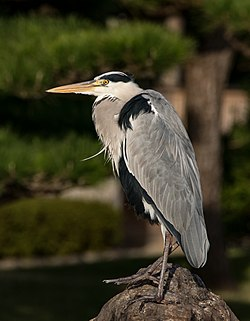
\includegraphics[width=0.8\linewidth, height=10cm, keepaspectratio]{Billeder/Dyr/Fugle/Hejrer/fiskehejre.jpg}
\end{minipage}
}%
\end{columns}
\end{frame}
% ========== TITEL: GÆS ==========
\begin{frame}
  \vspace{1.5em}
  \begin{center}
    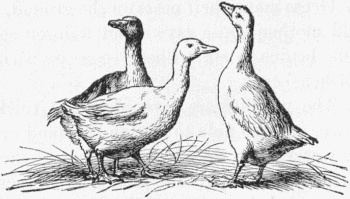
\includegraphics[width=12cm, height=4cm, keepaspectratio]{Billeder/Dyr/Fugle/Gaes/gæs.jpg}\\[1.2em]
    {\LARGE \textbf{Gæs}}\\[0.6em]
    
    Artsbestemmelse \&  vildtbiologi \\[0.9em]
    {\tiny\color{gray}
    CC BY 4.0 – kan frit anvendes, også kommercielt. Rettighederne må ikke skærpes.\\[0.05em]
    Udviklet af Aleksander Sønder, OSJAGTTEGN.DK}
  \end{center}
\end{frame}

% ========== GRÅGÅS ==========
\begin{frame}{%
  \begin{minipage}[c]{0.30\textwidth}
    Grågås
  \end{minipage}%
  \hfill
  \begin{minipage}[c]{0.45\textwidth}
    \footnotesize
    \textbf{Jagttid:} 1.\ sep.--31.\ jan. samt 1.\--31.\ aug.* \\
    \textbf{Regulering:} Efter aftale: 1.\--31.\ jul. \& 1.\--29.\ jan.
  \end{minipage}%
  \hfill
  \begin{minipage}[c]{0.15\textwidth}
    \noindent\raggedleft
    
\includegraphics[width=0.5cm, height=0.5cm, keepaspectratio]{Billeder/Ikoner/star.png}%
    \hspace{0.2em}%
    
\includegraphics[width=0.5cm, height=0.5cm, keepaspectratio]{Billeder/Ikoner/star.png}%
    \hspace{0.2em}%
    
\includegraphics[width=0.5cm, height=0.5cm, keepaspectratio]{Billeder/Ikoner/star.png}
  \end{minipage}%
}
  \vspace{0.25em}
  \begin{columns}[T]
    % --- Venstre kolonne: Tekst ---
    \column{0.45\textwidth}
    \setlength{\parskip}{0.5em}
    \tiny
    \RaggedRight
    \textbf{\textit{Anser anser}} – største af de grå gæs \par
    \textbf{Udseende:}\\
    \quad – Kødfarvede ben \\
    \quad – Kraftig hals \\
    \quad – Orangerødt næb \par
    \textbf{Levesteder:} Nær vådområder og på marker. \par
    \textbf{Føde:} Planteføde. \par
    \textbf{Udbredelse:} Hele Danmark. \par
    \textbf{Træk/standfugl:} Begge \par
    \textbf{Forplantning:}\\
    \quad – \textbf{Yngleforhold:} Yngler i hele Danmark \\
    \quad – \textbf{Kønsmoden:} Ca. 3 år \\
    \quad – \textbf{Mono/polygam:} Monogam \\
    \quad – \textbf{Bestandsomsætning:} Langsom \\
    \quad – \textbf{Kuld:} 4–6 æg
    \par
    \textbf{* Jagttid 1. - 31. august:} \\
    \quad – \textbf{Krav} På arealer i omdrift (aktive marker/landbrug) med minimumsafstand på 300m til ferske vandre større end 3ha
    % --- Højre kolonne: Større billede ---
    \column{0.52\textwidth}
    \centering
    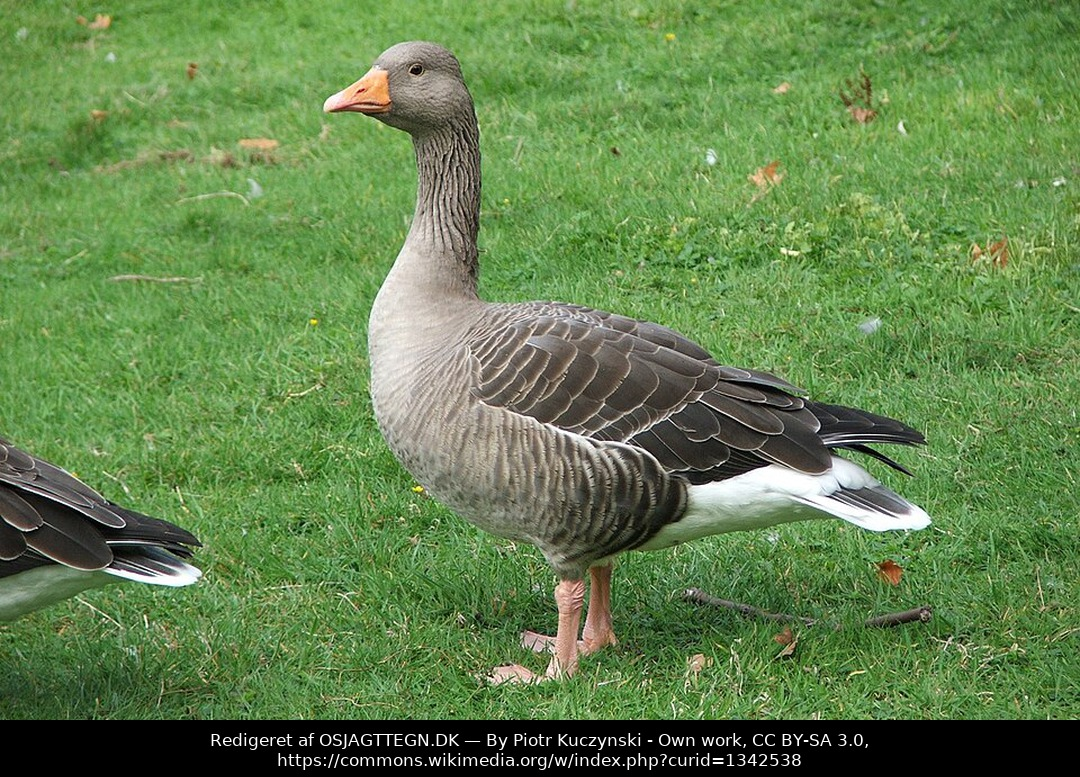
\includegraphics[width=\linewidth, height=7.2cm, keepaspectratio]{Billeder/Dyr/Fugle/Gaes/grågås.jpg}
  \end{columns}
\end{frame}
% ========== KNORTEGÅS ==========
\begin{frame}{%
  \begin{minipage}[c]{0.30\textwidth}
    Knortegås
  \end{minipage}%
  \hfill
  \begin{minipage}[c]{0.45\textwidth}
    \footnotesize
    \textbf{Jagttid:} Ingen jagttid
  \end{minipage}%
  \hfill
  \begin{minipage}[c]{0.15\textwidth}
    \noindent\raggedleft
    
\includegraphics[width=0.5cm, height=0.5cm, keepaspectratio]{Billeder/Ikoner/star.png}%
    \hspace{0.2em}%
    
\includegraphics[width=0.5cm, height=0.5cm, keepaspectratio]{Billeder/Ikoner/star.png}
  \end{minipage}%
}
  \vspace{0.25em}
  \begin{columns}[T]
    % --- Venstre kolonne: Tekst ---
    \column{0.45\textwidth}
    \setlength{\parskip}{0.5em}
    \tiny
    \RaggedRight
    \textbf{\textit{Branta bernicla}} – lille rajgås hvor navnet refererer til deres knurrende kald \par
    \textbf{Udseende:}\\
    \quad – Mørk med hvid halsring \par
    \textbf{Levesteder:} Kyster og fjorde. \par
    \textbf{Føde:} Ålegræs. \par
    \textbf{Udbredelse:} Overvintrer langs kysterne i Danmark. \par
    \textbf{Træk/standfugl:} Trækfugl
    % --- Højre kolonne: Større billede ---
    \column{0.52\textwidth}
    \centering
    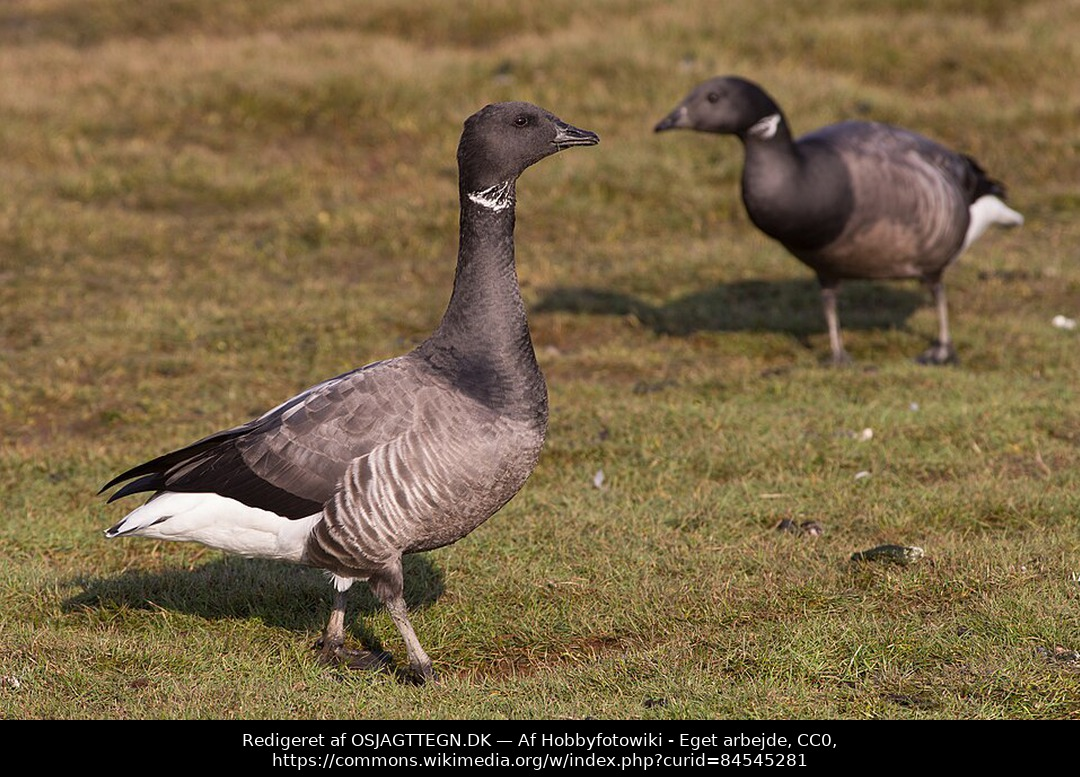
\includegraphics[width=\linewidth, height=7.2cm, keepaspectratio]{Billeder/Dyr/Fugle/Gaes/knortegås.jpg}
  \end{columns}
\end{frame}
% ========== KORTNÆBBET GÅS ==========
\begin{frame}{%
  \begin{minipage}[c]{0.30\textwidth}
    Kortnæbbet gås
  \end{minipage}%
  \hfill
  \begin{minipage}[c]{0.45\textwidth}
    \footnotesize
    \textbf{Jagttid:} 1.\ september -- 31.\ januar
  \end{minipage}%
  \hfill
  \begin{minipage}[c]{0.15\textwidth}
    \noindent\raggedleft
    
\includegraphics[width=0.5cm, height=0.5cm, keepaspectratio]{Billeder/Ikoner/star.png}%
    \hspace{0.2em}%
    
\includegraphics[width=0.5cm, height=0.5cm, keepaspectratio]{Billeder/Ikoner/star.png}
  \end{minipage}%
}
  \vspace{0.25em}
  \begin{columns}[T]
    % --- Venstre kolonne: Tekst ---
    \column{0.45\textwidth}
    \setlength{\parskip}{0.5em}
    \tiny
    \RaggedRight
    \textbf{\textit{Anser brachyrhynchus}} – kendes på det korte næb, men forveksles let med de øvrige grå gæs \par
    \textbf{Udseende:}\\
    \quad – Kort kraftigt lyserødt næb, lyserøde ben \par
    \textbf{Levesteder:} Vådområder og landbrugsarealer. \par
    \textbf{Føde:} Planteføde. \par
    \textbf{Udbredelse:} Langs vestkysten som trækfugl. \par
    \textbf{Træk/standfugl:} Trækfugl
    % --- Højre kolonne: Større billede ---
    \column{0.52\textwidth}
    \centering
    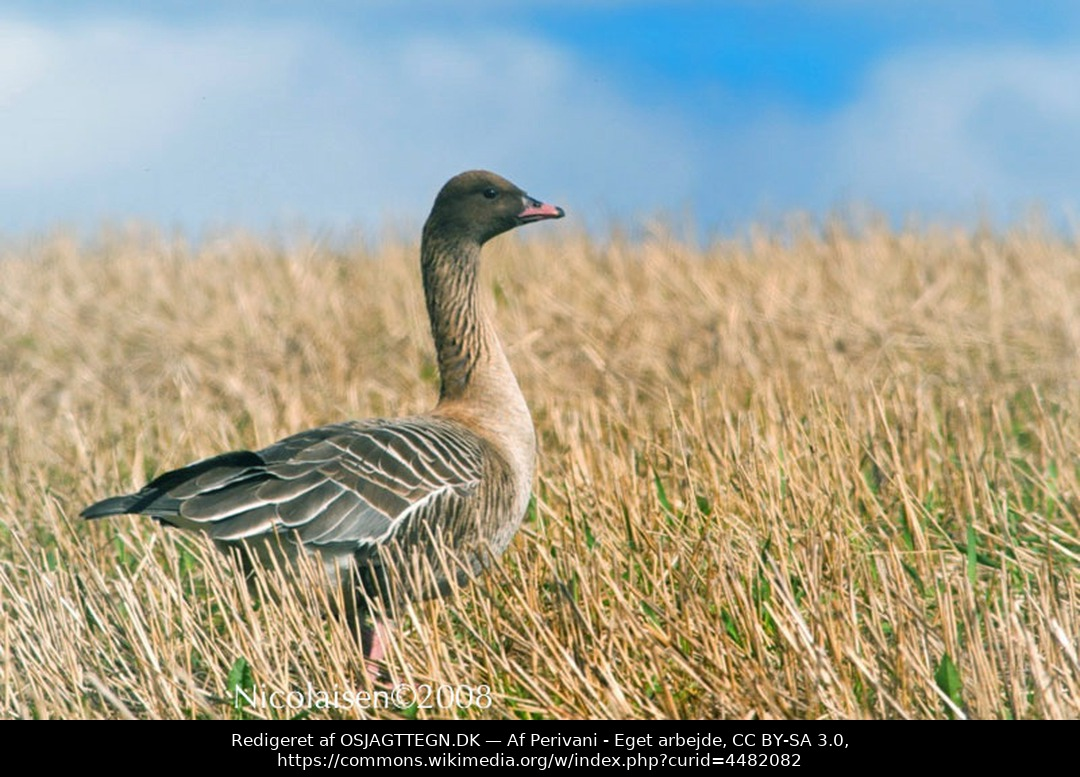
\includegraphics[width=\linewidth, height=7.2cm, keepaspectratio]{Billeder/Dyr/Fugle/Gaes/kortnæbbet_gås.jpg}
  \end{columns}
\end{frame}
% ========== SÆDGÅS ==========
\begin{frame}{%
  \begin{minipage}[c]{0.30\textwidth}
    Sædgås
  \end{minipage}%
  \hfill
  \begin{minipage}[c]{0.45\textwidth}
    \footnotesize
    \textbf{Jagttid:} Ingen jagttid
  \end{minipage}%
  \hfill
  \begin{minipage}[c]{0.15\textwidth}
    \noindent\raggedleft
    
\includegraphics[width=0.5cm, height=0.5cm, keepaspectratio]{Billeder/Ikoner/star.png}
  \end{minipage}%
}
  \vspace{0.25em}
  \begin{columns}[T]
    % --- Venstre kolonne: Tekst ---
    \column{0.45\textwidth}
    \setlength{\parskip}{0.5em}
    \tiny
    \RaggedRight
    \textbf{\textit{Anser fabalis}} – i familien "grå gæs" \par
    \textbf{Udseende:}\\
    \quad – Næb er orangegult, orangegule ben
    % --- Højre kolonne: Større billede ---
    \column{0.52\textwidth}
    \centering
    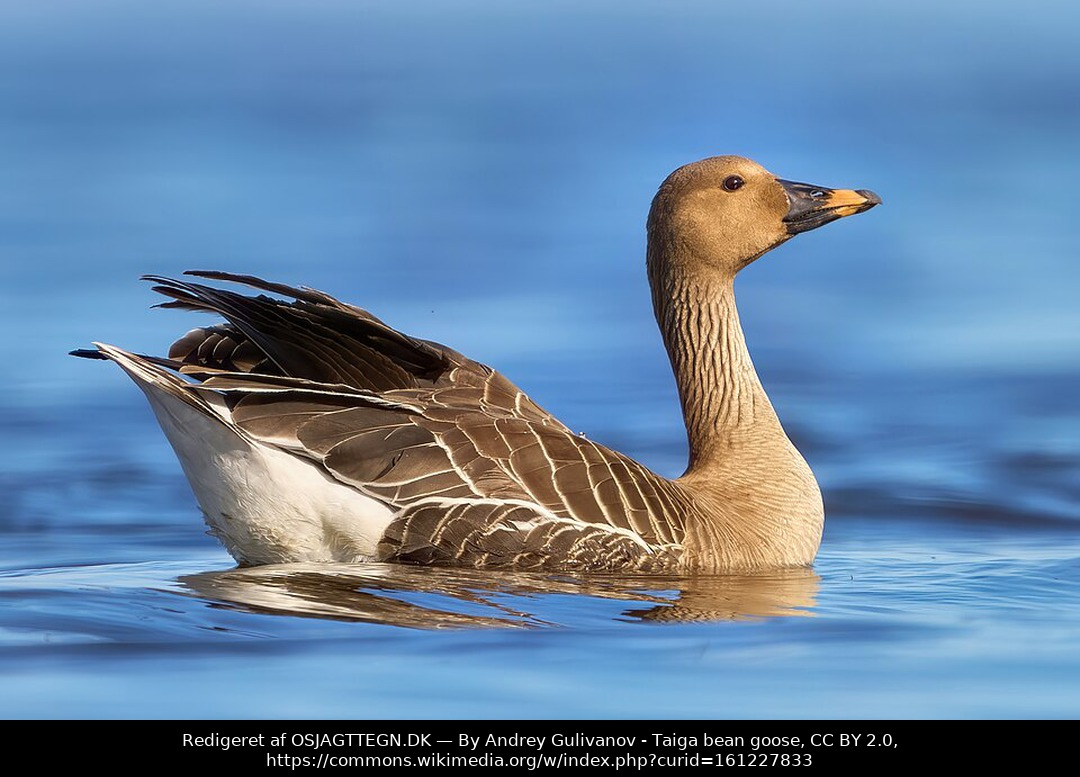
\includegraphics[width=\linewidth, height=7.2cm, keepaspectratio]{Billeder/Dyr/Fugle/Gaes/sædgås.jpg}
  \end{columns}
\end{frame}
% ========== BLISGÅS ==========
\begin{frame}{%
  \begin{minipage}[c]{0.30\textwidth}
    Blisgås
  \end{minipage}%
  \hfill
  \begin{minipage}[c]{0.45\textwidth}
    \footnotesize
    \textbf{Jagttid:} 1.\ september -- 31.\ januar
  \end{minipage}%
  \hfill
  \begin{minipage}[c]{0.15\textwidth}
    \noindent\raggedleft
    
\includegraphics[width=0.5cm, height=0.5cm, keepaspectratio]{Billeder/Ikoner/star.png}
  \end{minipage}%
}
  \vspace{0.25em}
  \begin{columns}[T]
    % --- Venstre kolonne: Tekst ---
    \column{0.45\textwidth}
    \setlength{\parskip}{0.5em}
    \tiny
    \RaggedRight
    \textbf{\textit{Anser albifrons}} – i familien "grå gæs" \par
    \textbf{Udseende:}\\
    \quad – Hvid blis ved næbroden, lyserødt næb, orange ben
    % --- Højre kolonne: Større billede ---
    \column{0.52\textwidth}
    \centering
    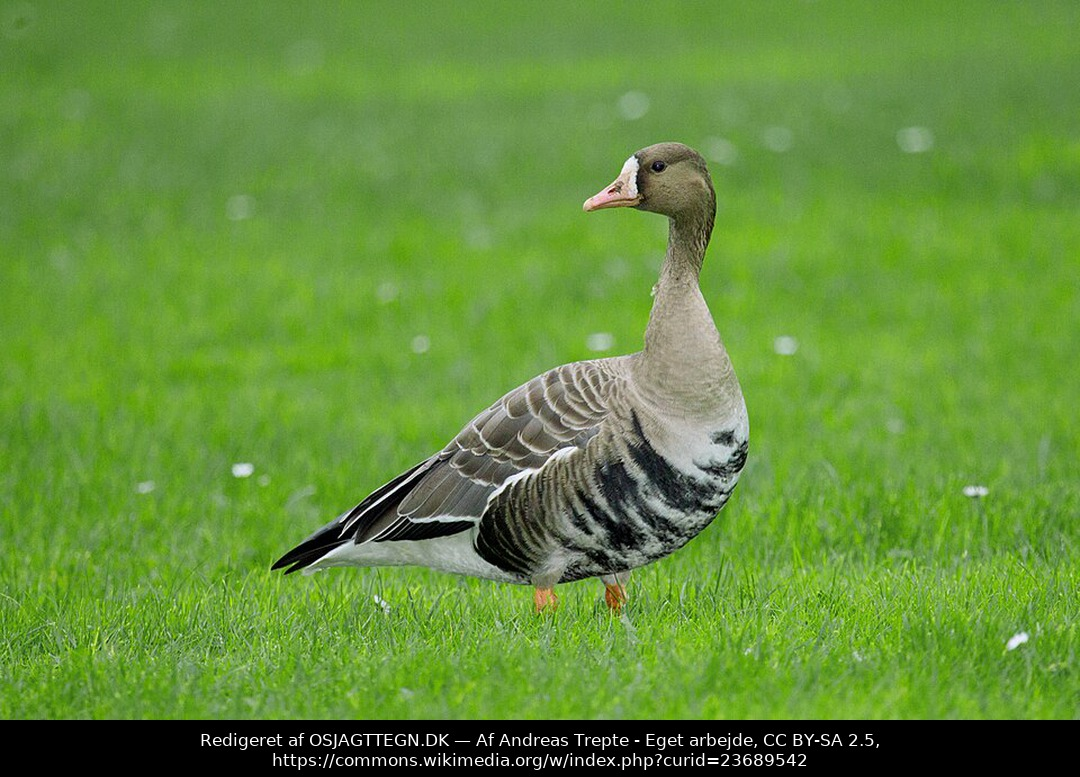
\includegraphics[width=\linewidth, height=7.2cm, keepaspectratio]{Billeder/Dyr/Fugle/Gaes/blisgås.jpg}
  \end{columns}
\end{frame}
% ========== BRAMGÅS ==========
\begin{frame}{%
  \begin{minipage}[c]{0.30\textwidth}
    Bramgås
  \end{minipage}%
  \hfill
  \begin{minipage}[c]{0.45\textwidth}
    \footnotesize
    \textbf{Jagttid:} Ingen jagttid
  \end{minipage}%
  \hfill
  \begin{minipage}[c]{0.15\textwidth}
    \noindent\raggedleft
    
\includegraphics[width=0.5cm, height=0.5cm, keepaspectratio]{Billeder/Ikoner/star.png}
  \end{minipage}%
}
  \vspace{0.25em}
  \begin{columns}[T]
    % --- Venstre kolonne: Tekst ---
    \column{0.45\textwidth}
    \setlength{\parskip}{0.5em}
    \tiny
    \RaggedRight
    \textbf{\textit{Branta leucopsis}} – lille rajgås som er i familie med knortegås og canadagås \par
    \textbf{Udseende:}\\
    \quad – Hvid kindplet der dækker det meste af hovedet
    % --- Højre kolonne: Større billede ---
    \column{0.52\textwidth}
    \centering
    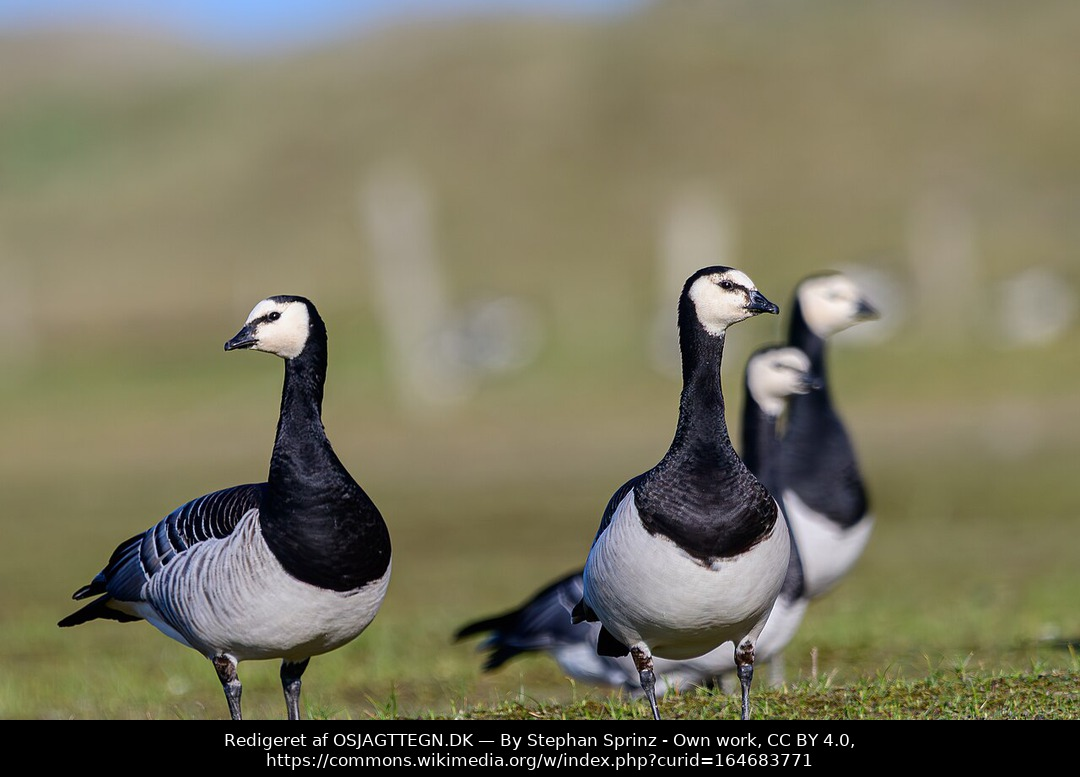
\includegraphics[width=\linewidth, height=7.2cm, keepaspectratio]{Billeder/Dyr/Fugle/Gaes/bramgås.jpg}
  \end{columns}
\end{frame}
% ========== CANADAGÅS ==========
\begin{frame}{%
  \begin{minipage}[c]{0.30\textwidth}
    Canadagås
  \end{minipage}%
  \hfill
  \begin{minipage}[c]{0.45\textwidth}
    \footnotesize
    \textbf{Jagttid:} 1.\ sep. -- 31.\ jan. samt 1.\ -- 31.\ aug.*
  \end{minipage}%
  \hfill
  \begin{minipage}[c]{0.15\textwidth}
    \noindent\raggedleft
    
\includegraphics[width=0.5cm, height=0.5cm, keepaspectratio]{Billeder/Ikoner/star.png}
  \end{minipage}%
}
  \vspace{0.25em}
  \begin{columns}[T]
    % --- Venstre kolonne: Tekst ---
    \column{0.45\textwidth}
    \setlength{\parskip}{0.5em}
    \tiny
    \RaggedRight
    \textbf{\textit{Branta canadensis}} – større hjemmehørende gås i rajgæs-familien \par
    \textbf{Udseende:}\\
    \quad – Stor krop og hvid plet bag øjet på kinden
    \par
    \textbf{* Jagttid 1. - 31. august:} \\
    \quad – \textbf{Krav} På arealer i omdrift (aktive marker/landbrug) med minimumsafstand på 300m til ferske vandre større end 3ha
    % --- Højre kolonne: Større billede ---
    \column{0.52\textwidth}
    \centering
    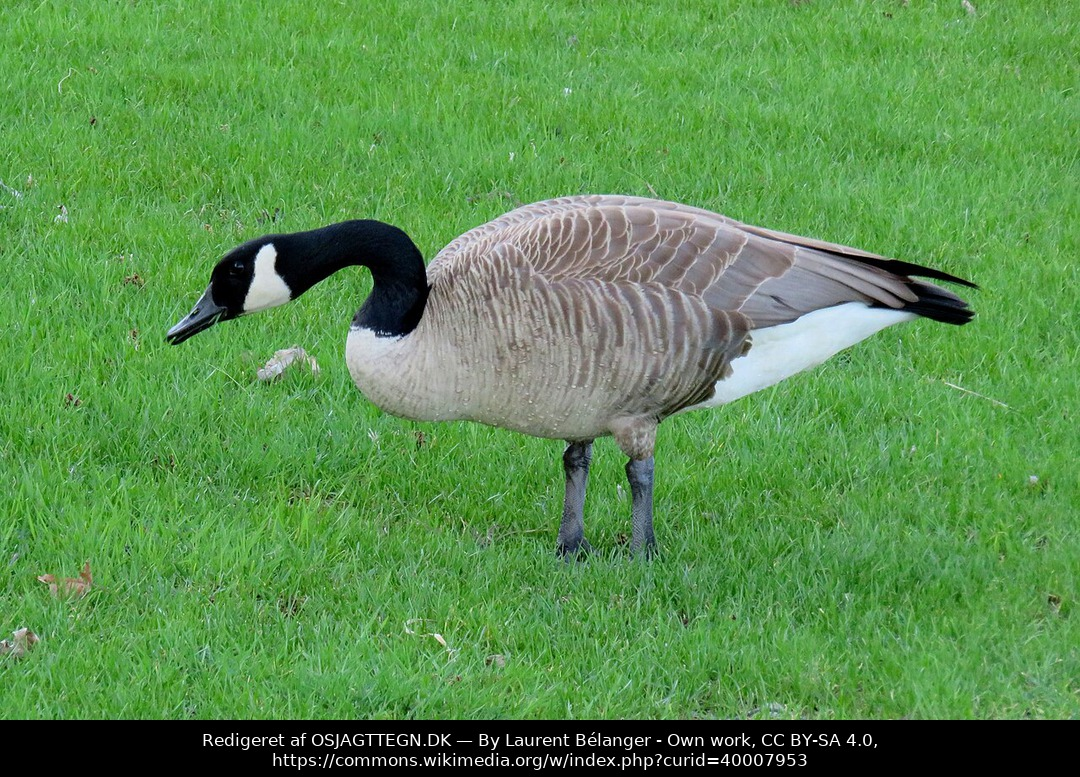
\includegraphics[width=\linewidth, height=7.2cm, keepaspectratio]{Billeder/Dyr/Fugle/Gaes/canadagås.jpg}
  \end{columns}
\end{frame}
\section{Våbenhåndtering}

\begin{frame}
  \vspace{3em}
  \begin{center}
    {\LARGE \textbf{Våbenhåndtering}}
  \end{center}
\end{frame}

\begin{frame}{Våbenhåndtering – en proces}
  \vspace{1em}
  \begin{columns}[T]
    \column{0.05\textwidth}

    \column{0.9\textwidth}
    \setlength{\parskip}{0.6em}
    \small
    \RaggedRight

    \textbf{Våbenhåndtering er en proces} – \\
    adskilt i klare, rolige faser. \par

    \vspace{0.6em}
    \textbf{Hver fase skal være:} \\
    \quad – Håndfast \\
    \quad – Rolig \\
    \quad – Afsluttet \\
    \quad – Bevidst \par

    \vspace{0.6em}
    \textit{Først når en fase er fuldt gennemført, \\
    iværksættes næste fase.} \par

    

    \column{0.05\textwidth}
  \end{columns}
\end{frame}

\begin{frame}{Våbenhåndtering – trin for trin}
  \vspace{0.2em}
  \begin{columns}[T]
    % --- Venstre kolonne: Opstart + Forhindring ---
    \column{0.48\textwidth}
    \setlength{\parskip}{0.32em}
    \footnotesize
    \RaggedRight

    \textbf{-- Opstart --} \\
    1. Fødder i skudretning – fri for mennesker. \\
    2. Forskæfte med \textit{modsatte hånd} af skulderen du vil lægge geværet til. \\
    3. Åbn geværet lodret med topnøgle. \\
    4. Kig igennem – \textit{tomt og rent}. \\
    5. Før gennem vandret (knækket). \\
    6. Isæt patroner. \\
    7. Luk i \textbf{45°} – hør \textit{klik}. \\
    8. Før op til \textit{semi-klar}.. \\
    9. \textit{Fingre væk} fra aftrækker/sikring. \par

    \vspace{0.4em}
    \textbf{-- Forhindring --} \\
    10. Før geværet ned gennem vandret. \\
    11. Åbn – patroner \textit{i lommen}. \\
    12. Forcer med \textit{knækket gevær}. \\
    13. Efterse løbene. \\
    14. Isæt patroner igen. \\
    15. Før op gennem vandret. \par

    % --- Højre kolonne: Skudafgivelse ---
    \column{0.48\textwidth}
    \setlength{\parskip}{0.32em}
    \footnotesize
    \RaggedRight

    \textbf{-- Skudafgivelse --} \\
    16. Geværet lades \\
    17. Op til \textit{semi-klar}. \\
    18. Kolbe mod bryst – nær armhule. Min 30° \\
    19. Meld: \textbf{„KLAR!“} \\
    20. Afsikring \textit{frem}. \\
    21. Affyr 1–2 skud. \\
    22. Ned til bryst. \\
    23. Sikring \textit{tilbage}. \\
    24. Ned gennem vandret. \\
    25. Åbn – fjern afskudte. \\
    26. Gentag \textbf{4 gange}. \\
    27. Aflever \textit{alle patroner}. \par

  \end{columns}
\end{frame}

\begin{frame}
  \vspace{3em}
  \begin{center}
    {\LARGE \textbf{Gå sammen to og to}} \\
    {\LARGE \textbf{Fuldfør steps med klikpatroner}}
  \end{center}
\end{frame}
\section{Jagt fra kunstige skjul}

\begin{frame}
  \vspace{3em}
  \begin{center}
    {\LARGE \textbf{Jagt fra kunstige skjul}
    }
    \\
    \vspace{1em}
    Bekendtgørelse om udsætning af vildt, jagtmåder og jagtredskaber
    \\
    \vspace{1em}
    BEK nr 1652 af 19/12/2017, Kapitel 1
  \end{center}
\end{frame}

\begin{frame}
    \frametitle{Forbud mod jagt på pattedyr fra kunstige skjul (§ 1)}

    \vspace{1.5cm}

    § 1

    \vspace{0.5cm}

    Der må ikke drives jagt på pattedyr fra

    \vspace{0.5cm}

    1) kunstigt skjul, herunder hus, hytte, jordhul, eller

    \vspace{0.5cm}

    2) platform eller sæde, der er hævet mere end 50 cm over det omgivende terræn.

    \vspace{0.5cm}

    Med to undtagelser

    \vspace{2.5cm}
\end{frame}

\begin{frame}
    \frametitle{Varianter af kunstige skjul}

    \begin{columns}
        \column{0.5\textwidth}
        \centering
        \begin{figure}
            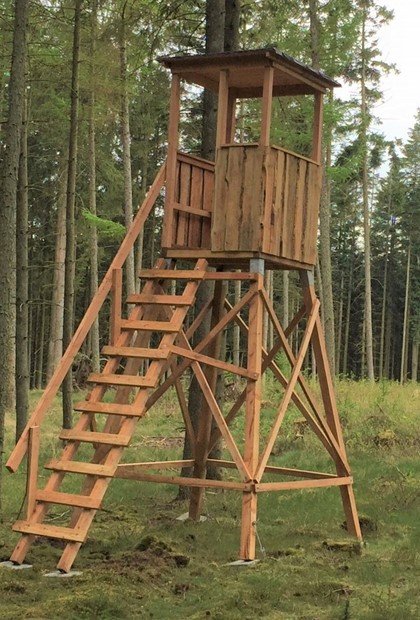
\includegraphics[width=0.5\textwidth]{Billeder/Redskaber/jagttårn.jpg}
            \caption{\textbf{Jagttårn} (jægeren kan skyde stående)}
        \end{figure}
        
        \column{0.5\textwidth}
        \centering
        \begin{figure}
            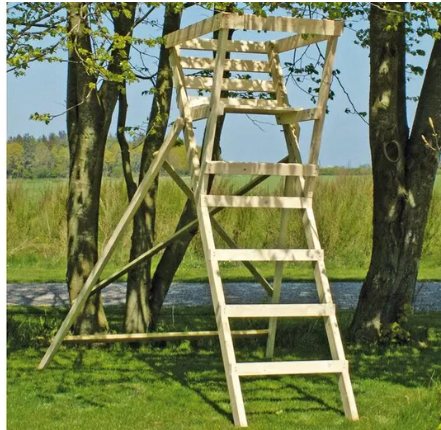
\includegraphics[width=0.5\textwidth]{Billeder/Redskaber/jagtstige.png}
            \caption{\textbf{Jagtstige} (jægeren kan skyde siddende)}
        \end{figure}
    \end{columns}

    \vspace{1cm}  % Plads til tekst under

    \centering
\end{frame}

\begin{frame}
    \frametitle{Regler for skydetårne (§ 1)}

    \begin{columns}[T]  % T for top-alignment
        \column{0.6\textwidth}
        \begin{itemize}
            \item Højere end 50 cm over omkringliggende areal
            \item Min 130 m til skel med mindre andet er aftalt skriftligt
            \item Udført i træ eller metal
            \item Opsættes i min 0,5 hektar skov eller ydre/inde skovbryn
            \item Må ikke skæmme (samme højde som øvrig bevoksning)
            \item Højde til plateau max 5m
            \item Sider max 110cm høje
            \item Plateau max 2 $m^2$
            \item Tag i et plan, ikke-reflekterende, max 10 cm udhæng
        \end{itemize}
        
        \column{0.4\textwidth}
        \centering
        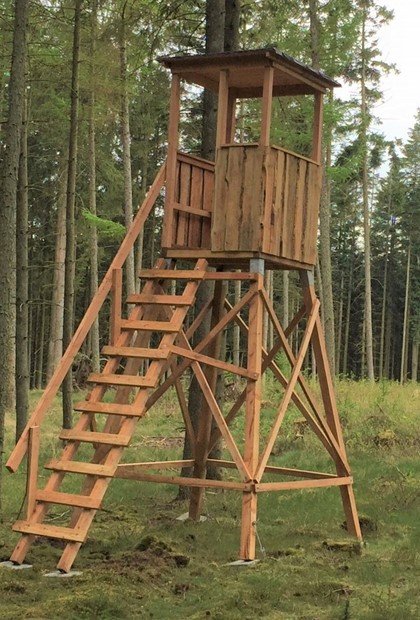
\includegraphics[width=0.7\textwidth]{Billeder/Redskaber/jagttårn.jpg}  % Mindre billede nu
        \vspace{0.5cm}
        \small 
    \end{columns}

\end{frame}

\begin{frame}
    \frametitle{Regler for skydestiger (§ 1)}

    \begin{columns}[T]  % T for top-alignment
        \column{0.6\textwidth}
        \begin{itemize}
            \item Højere end 50 cm over omkringliggende areal
            \item Min 130 m til skel med mindre andet er aftalt skriftligt
            \item De skal være mobile eller midlertidige konstruktioner
            \item Opsættes i hegn eller bevoksninger (ikke 0,5 hektar regel)
            \item Må ikke skæmme (samme højde som øvrig bevoksning)
            \item Højde til plateau max 5 m
        \end{itemize}
        
        \column{0.4\textwidth}
        \centering
        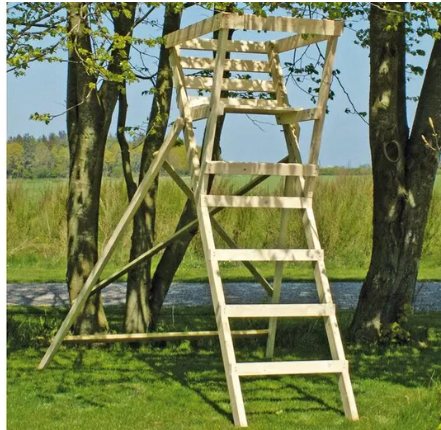
\includegraphics[width=0.7\textwidth]{Billeder/Redskaber/jagtstige.png}  % Mindre billede nu
        \vspace{0.5cm}
        \small 
    \end{columns}

    \end{frame}

\begin{frame}
    \frametitle{Regler for kunstige skjul på fugle (§ 3)}

    \begin{columns}[T]  % T for top-alignment
        \column{0.6\textwidth}
        \begin{itemize}
            \item Gulvet/ståstedet må højest være hævet 50 cm over terrænnet
            \item Ellers er kreativiteten ubegrænset – brug camouflage, net, siv, grene osv.
            \item Skjulet kan være midlertidigt (flytbart) eller mere fast (f.eks. ramme med net)
            \item Ofte brugt til andejagt, duejagt eller kragejagt med lokkefugle
            \item Husk at våbentype skal passe til skjulet (typisk haglgevær til fugle) (§ 2)
            \item Skjulet skal camouflages godt for ikke at skræmme vildtet
        \end{itemize}
        
        \column{0.4\textwidth}
        \centering
        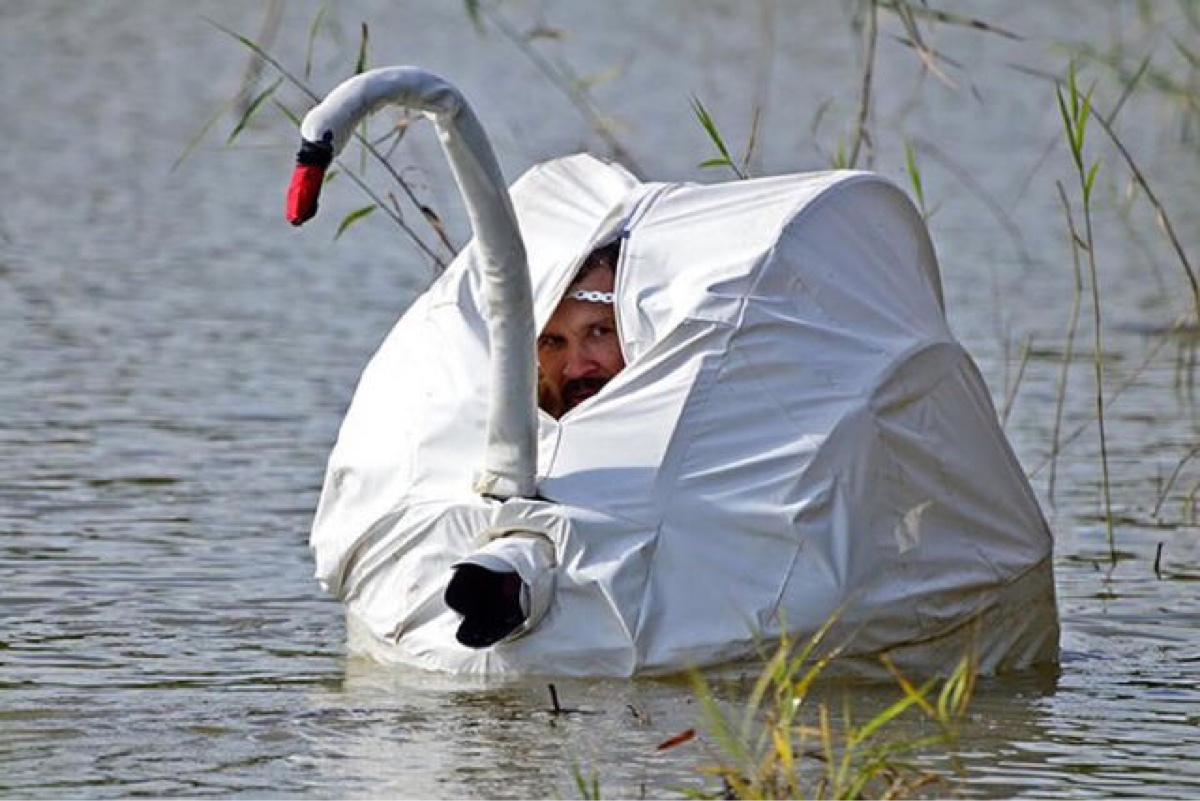
\includegraphics[width=0.9\textwidth]{Billeder/Redskaber/kunstigtskjul.jpg}
        \vspace{0.5cm}
        
    \end{columns}

\end{frame}

\section{Rovfugle (vildtkending og biologi)}

\begin{frame}
  \vspace{1.5em}
  \begin{center}
    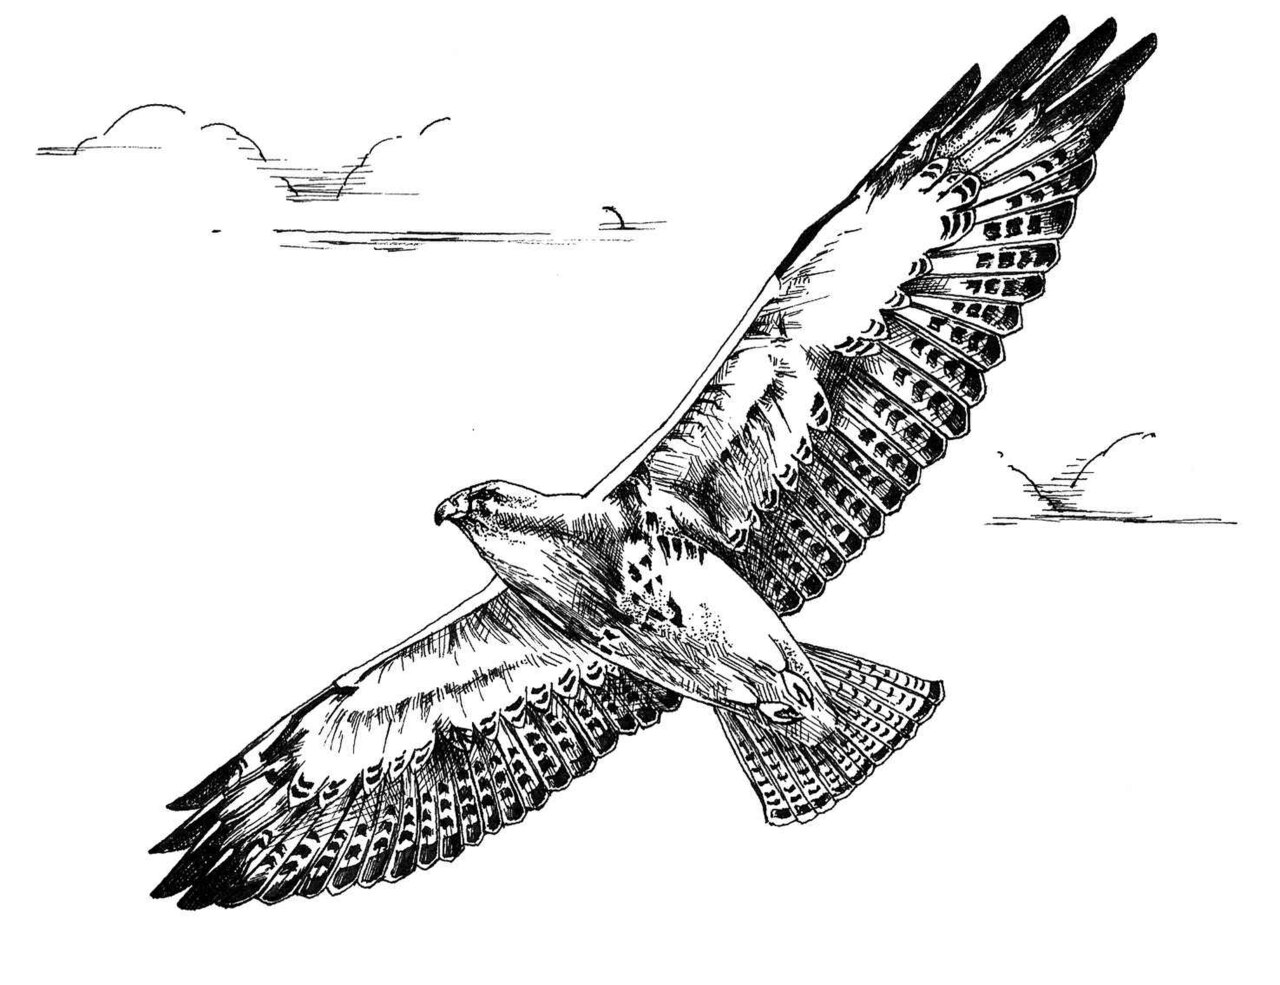
\includegraphics[width=12cm, height=4cm, keepaspectratio]{Billeder/Dyr/Fugle/Rovfugle/rovfugle.jpg}\\[1.2em]
    {\LARGE \textbf{Rovfugle}}
    \vspace{1em}
    \\ Artsbestemmelse og vildtbiologi
    \\[0.9em]
    {\tiny\color{gray}
    CC BY 4.0 – kan frit anvendes, også kommercielt. Rettighederne må ikke skærpes.\\[0.05em]
    Udviklet af Aleksander Sønder, OSJAGTTEGN.DK}
  \end{center}
\end{frame}

% ========== MUSVÅGE ==========
\begin{frame}{%
  \begin{minipage}[c]{0.30\textwidth}
    Musvåge
  \end{minipage}%
  \hfill
  \begin{minipage}[c]{0.45\textwidth}
    \footnotesize
    \textbf{Jagttid:} Ingen jagttid
  \end{minipage}%
  \hfill
  \begin{minipage}[c]{0.15\textwidth}
    \noindent\raggedleft
    
\includegraphics[width=0.5cm, height=0.5cm, keepaspectratio]{Billeder/Ikoner/star.png}%
    \hspace{0.2em}%
    
\includegraphics[width=0.5cm, height=0.5cm, keepaspectratio]{Billeder/Ikoner/star.png}
  \end{minipage}%
}
  \vspace{0.25em}
  \begin{columns}[T]
    % --- Venstre kolonne: Tekst ---
    \column{0.45\textwidth}
    \setlength{\parskip}{0.5em}
    \tiny
    \RaggedRight
    \textbf{\textit{Buteo buteo}} – kraftig bredskuldret rovfugl med musende kald \par
    \textbf{Udseende:}\\
    \quad – Brun men kan variere fra mørk til lys. Spraglet bryst. \par
    \textbf{Levesteder:} Det åbne land. \par
    \textbf{Føde:} Mus, gnavere, orme, frøer, harekillinger. \par
    \textbf{Udbredelse:} Hele Danmark. \par
    \textbf{Træk/standfugl:} Begge
    % --- Højre kolonne: Større billede ---
    \column{0.52\textwidth}
    \centering
    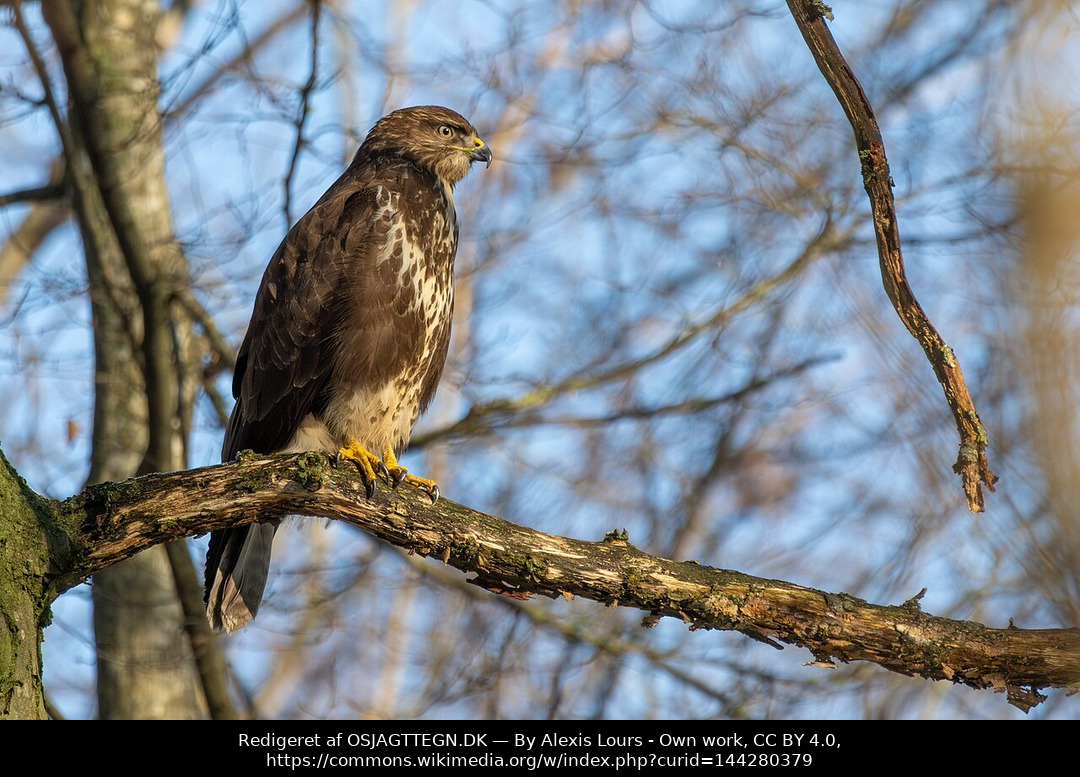
\includegraphics[width=\linewidth, height=7.2cm, keepaspectratio]{Billeder/Dyr/Fugle/Rovfugle/musvåge.jpg}
  \end{columns}
\end{frame}
% ========== SPURVEHØG ==========
\begin{frame}{%
  \begin{minipage}[c]{0.30\textwidth}
    Spurvehøg
  \end{minipage}%
  \hfill
  \begin{minipage}[c]{0.45\textwidth}
    \footnotesize
    \textbf{Jagttid:} Ingen jagttid
  \end{minipage}%
  \hfill
  \begin{minipage}[c]{0.15\textwidth}
    \noindent\raggedleft
    
\includegraphics[width=0.5cm, height=0.5cm, keepaspectratio]{Billeder/Ikoner/star.png}%
    \hspace{0.2em}%
    
\includegraphics[width=0.5cm, height=0.5cm, keepaspectratio]{Billeder/Ikoner/star.png}
  \end{minipage}%
}
  \vspace{0.25em}
  \begin{columns}[T]
    % --- Venstre kolonne: Tekst ---
    \column{0.45\textwidth}
    \setlength{\parskip}{0.5em}
    \tiny
    \RaggedRight
    \textbf{\textit{Accipiter nisus}} – relativt lille rovfugl \par
    \textbf{Udseende:}\\
    \quad – Tynde gule tændstiksben, rustrøde tværstriber på bryst \par
    \textbf{Levesteder:} Skovområder men forefindes også i byområder. \par
    \textbf{Føde:} Spurve og drosler som fanges ved overraskelse. \par
    \textbf{Udbredelse:} Hele Danmark. \par
    \textbf{Træk/standfugl:} Begge
    % --- Højre kolonne: Større billede ---
    \column{0.52\textwidth}
    \centering
    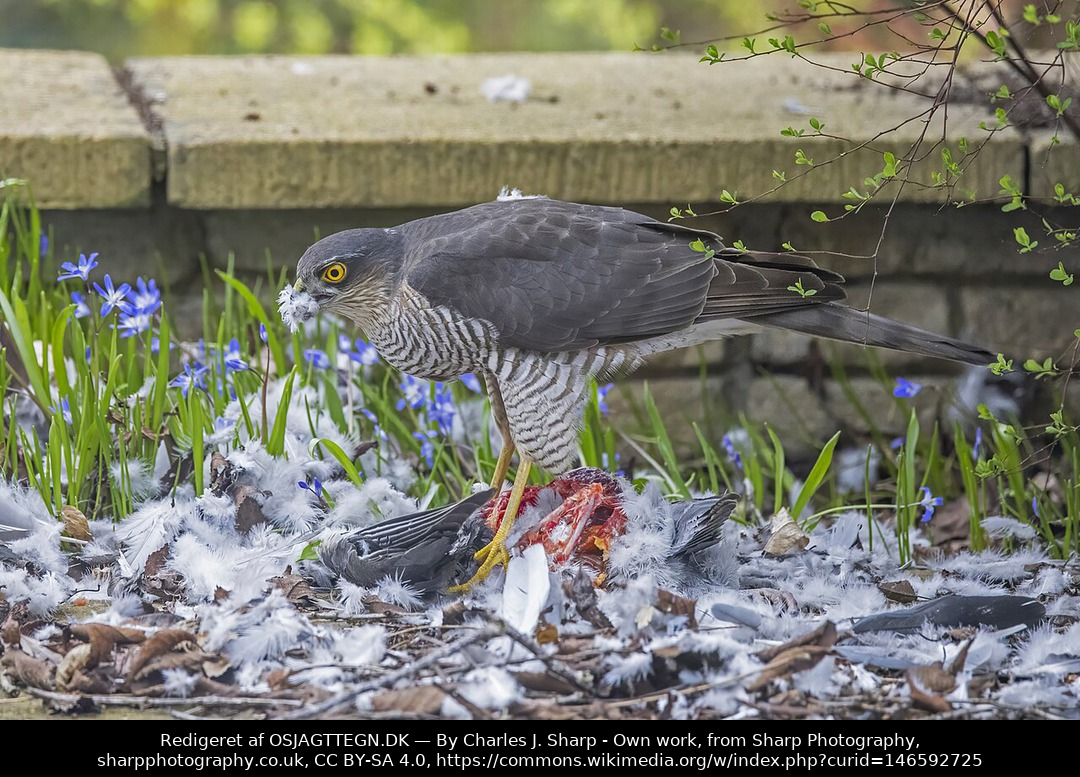
\includegraphics[width=\linewidth, height=7.2cm, keepaspectratio]{Billeder/Dyr/Fugle/Rovfugle/spurvehøg.jpg}
  \end{columns}
\end{frame}
% ========== TÅRNFALK ==========
\begin{frame}{%
  \begin{minipage}[c]{0.30\textwidth}
    Tårnfalk
  \end{minipage}%
  \hfill
  \begin{minipage}[c]{0.45\textwidth}
    \footnotesize
    \textbf{Jagttid:} Ingen jagttid
  \end{minipage}%
  \hfill
  \begin{minipage}[c]{0.15\textwidth}
    \noindent\raggedleft
    
\includegraphics[width=0.5cm, height=0.5cm, keepaspectratio]{Billeder/Ikoner/star.png}%
    \hspace{0.2em}%
    
\includegraphics[width=0.5cm, height=0.5cm, keepaspectratio]{Billeder/Ikoner/star.png}
  \end{minipage}%
}
  \vspace{0.25em}
  \begin{columns}[T]
    % --- Venstre kolonne: Tekst ---
    \column{0.45\textwidth}
    \setlength{\parskip}{0.5em}
    \tiny
    \RaggedRight
    \textbf{\textit{Falco tinnunculus}} – en af de mest udbredte rovfugle i Danmark \par
    \textbf{Udseende:}\\
    \quad – Teglrød overside med pletter, mørke tværbånd på halen \par
    \textbf{Levesteder:} Åbne arealer, også i byer og langs veje. \par
    \textbf{Føde:} Mus, gnavere og insekter. \par
    \textbf{Udbredelse:} Hele Danmark. \par
    \textbf{Træk/standfugl:} Begge
    % --- Højre kolonne: Større billede ---
    \column{0.52\textwidth}
    \centering
    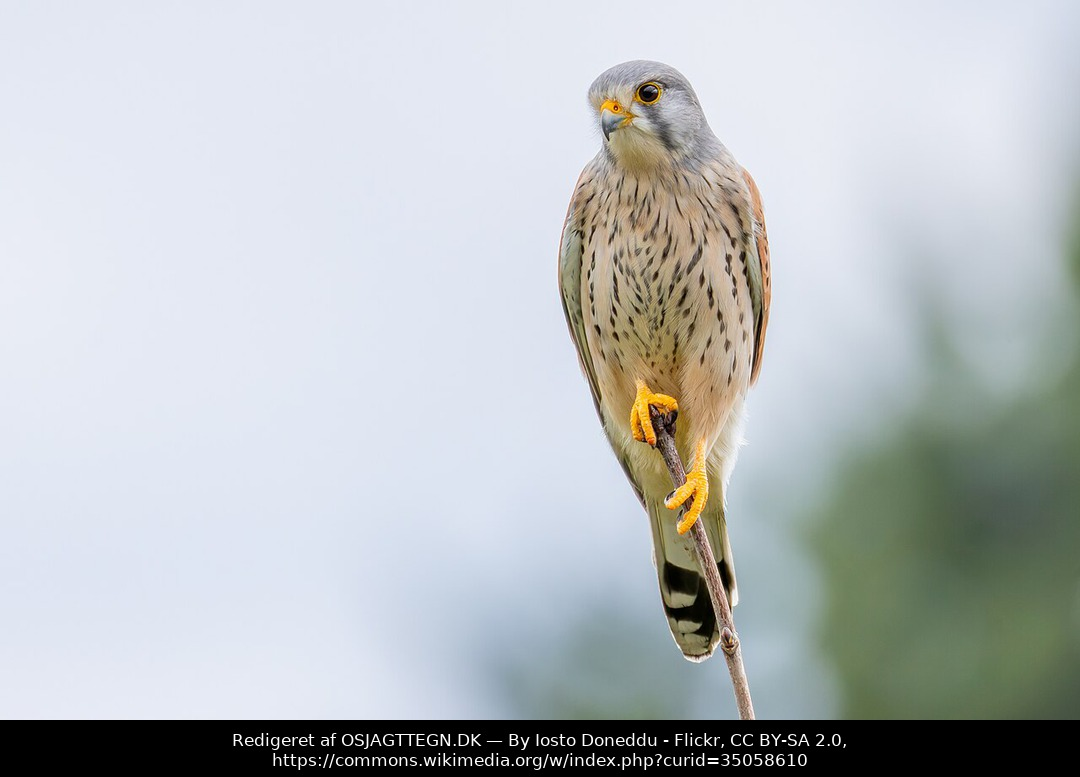
\includegraphics[width=\linewidth, height=7.2cm, keepaspectratio]{Billeder/Dyr/Fugle/Rovfugle/tårnfalk.jpg}
  \end{columns}
\end{frame}
% ========== DUEHØG ==========
\begin{frame}{%
  \begin{minipage}[c]{0.30\textwidth}
    Duehøg
  \end{minipage}%
  \hfill
  \begin{minipage}[c]{0.45\textwidth}
    \footnotesize
    \textbf{Jagttid:} Ingen jagttid
  \end{minipage}%
  \hfill
  \begin{minipage}[c]{0.15\textwidth}
    \noindent\raggedleft
    
\includegraphics[width=0.5cm, height=0.5cm, keepaspectratio]{Billeder/Ikoner/star.png}
  \end{minipage}%
}
  \vspace{0.25em}
  \begin{columns}[T]
    % --- Venstre kolonne: Tekst ---
    \column{0.45\textwidth}
    \setlength{\parskip}{0.5em}
    \tiny
    \RaggedRight
    \textbf{\textit{Accipiter gentilis}} – stor høg \par
    \textbf{Udseende:}\\
    \quad – Grå, med tværtstriber på bryst, lys øjenstribe
    % --- Højre kolonne: Større billede ---
    \column{0.52\textwidth}
    \centering
    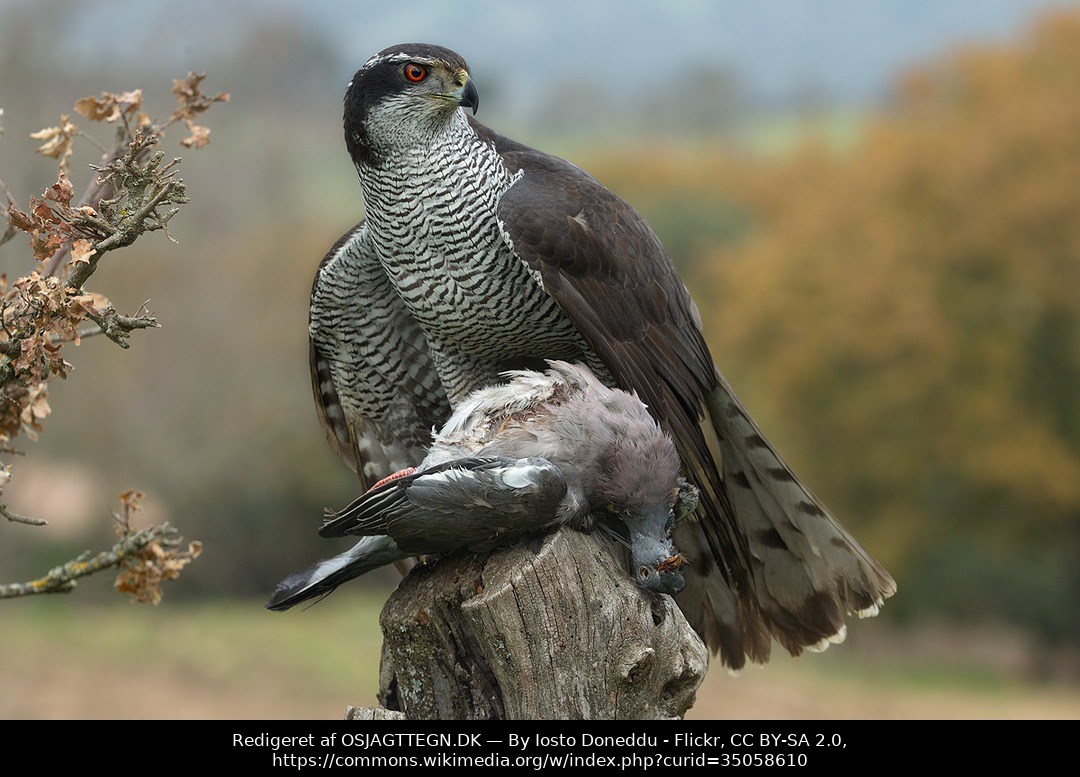
\includegraphics[width=\linewidth, height=7.2cm, keepaspectratio]{Billeder/Dyr/Fugle/Rovfugle/duehoeg.jpg}
  \end{columns}
\end{frame}
% ========== VANDREFALK ==========
\begin{frame}{%
  \begin{minipage}[c]{0.30\textwidth}
    Vandrefalk
  \end{minipage}%
  \hfill
  \begin{minipage}[c]{0.45\textwidth}
    \footnotesize
    \textbf{Jagttid:} Ingen jagttid
  \end{minipage}%
  \hfill
  \begin{minipage}[c]{0.15\textwidth}
    \noindent\raggedleft
    
\includegraphics[width=0.5cm, height=0.5cm, keepaspectratio]{Billeder/Ikoner/star.png}
  \end{minipage}%
}
  \vspace{0.25em}
  \begin{columns}[T]
    % --- Venstre kolonne: Tekst ---
    \column{0.45\textwidth}
    \setlength{\parskip}{0.5em}
    \tiny
    \RaggedRight
    \textbf{\textit{Falco peregrinus}} – mellemstor falk – kan flyve 150 km/t \par
    \textbf{Udseende:}\\
    \quad – Tynde tværstriber med sort pilothjelm. Bemærk skægstriben
    % --- Højre kolonne: Større billede ---
    \column{0.52\textwidth}
    \centering
    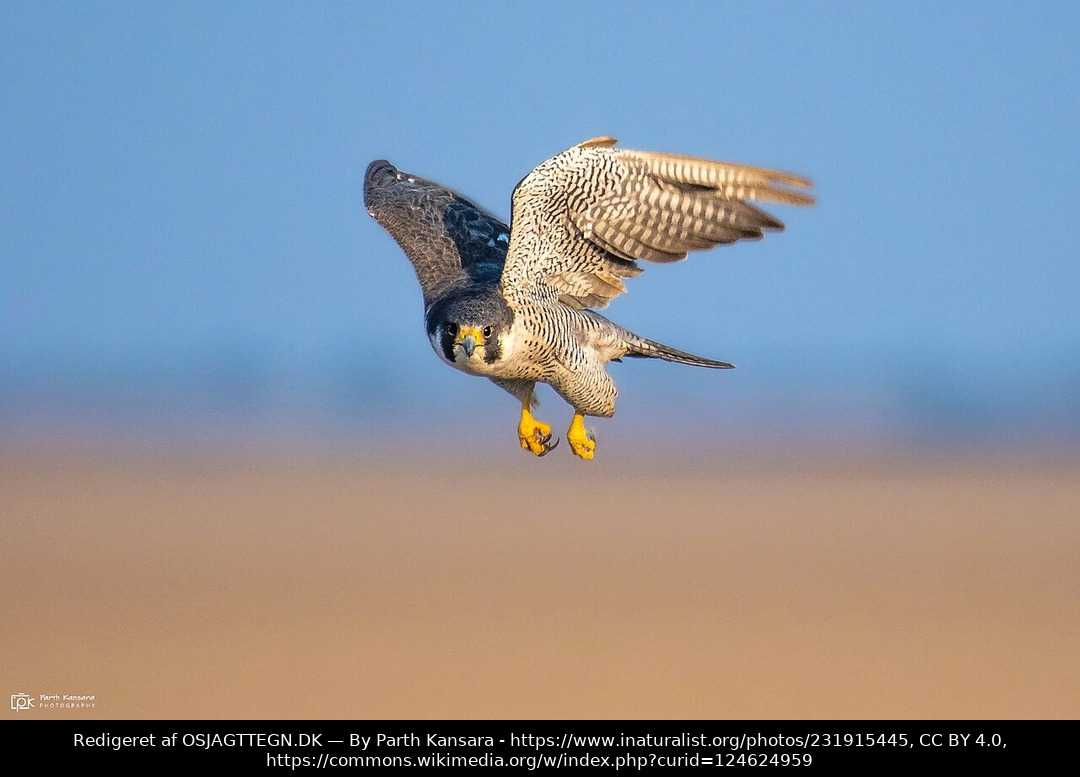
\includegraphics[width=\linewidth, height=7.2cm, keepaspectratio]{Billeder/Dyr/Fugle/Rovfugle/vandrefalk.jpg}
  \end{columns}
\end{frame}
% ========== RØRHØG ==========
\begin{frame}{%
  \begin{minipage}[c]{0.30\textwidth}
    Rørhøg
  \end{minipage}%
  \hfill
  \begin{minipage}[c]{0.45\textwidth}
    \footnotesize
    \textbf{Jagttid:} Ingen jagttid
  \end{minipage}%
  \hfill
  \begin{minipage}[c]{0.15\textwidth}
    \noindent\raggedleft
    
\includegraphics[width=0.5cm, height=0.5cm, keepaspectratio]{Billeder/Ikoner/star.png}
  \end{minipage}%
}
  \vspace{0.25em}
  \begin{columns}[T]
    % --- Venstre kolonne: Tekst ---
    \column{0.45\textwidth}
    \setlength{\parskip}{0.5em}
    \tiny
    \RaggedRight
    \textbf{\textit{Circus aeruginosus}} – i familien kærhøge som er kendetegnet ved v-formen i vingerne \par
    \textbf{Udseende:}\\
    \quad – Flødegult hovede og bryst, lange ben
    % --- Højre kolonne: Større billede ---
    \column{0.52\textwidth}
    \centering
    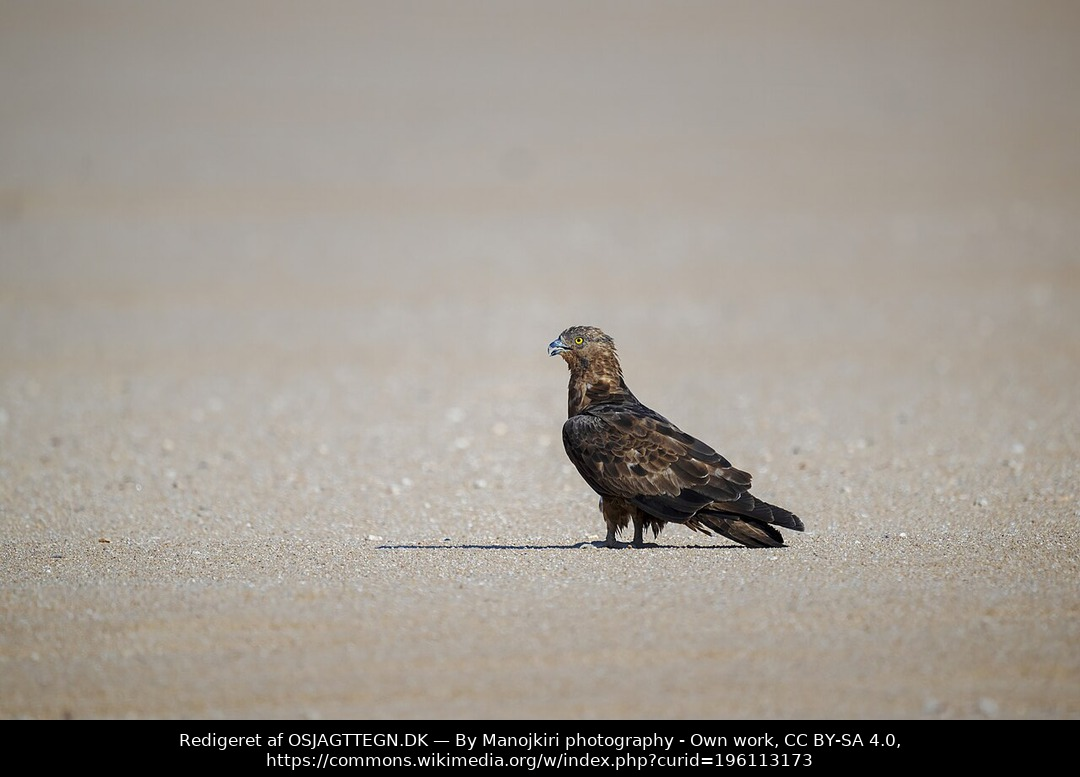
\includegraphics[width=\linewidth, height=7.2cm, keepaspectratio]{Billeder/Dyr/Fugle/Rovfugle/rørhøg.jpg}
  \end{columns}
\end{frame}
% ========== FISKEØRN ==========
\begin{frame}{%
  \begin{minipage}[c]{0.30\textwidth}
    Fiskeørn
  \end{minipage}%
  \hfill
  \begin{minipage}[c]{0.45\textwidth}
    \footnotesize
    \textbf{Jagttid:} Ingen jagttid
  \end{minipage}%
  \hfill
  \begin{minipage}[c]{0.15\textwidth}
    \noindent\raggedleft
    
\includegraphics[width=0.5cm, height=0.5cm, keepaspectratio]{Billeder/Ikoner/star.png}
  \end{minipage}%
}
  \vspace{0.25em}
  \begin{columns}[T]
    % --- Venstre kolonne: Tekst ---
    \column{0.45\textwidth}
    \setlength{\parskip}{0.5em}
    \tiny
    \RaggedRight
    \textbf{\textit{Pandion haliaetus}} – mellemstor rovfugl med lange smalle vinger \par
    \textbf{Udseende:}\\
    \quad – Grå overside, hvid underside. Hvidt hoved med sort stribe langsgående med halsen. Blå ben
    % --- Højre kolonne: Større billede ---
    \column{0.52\textwidth}
    \centering
    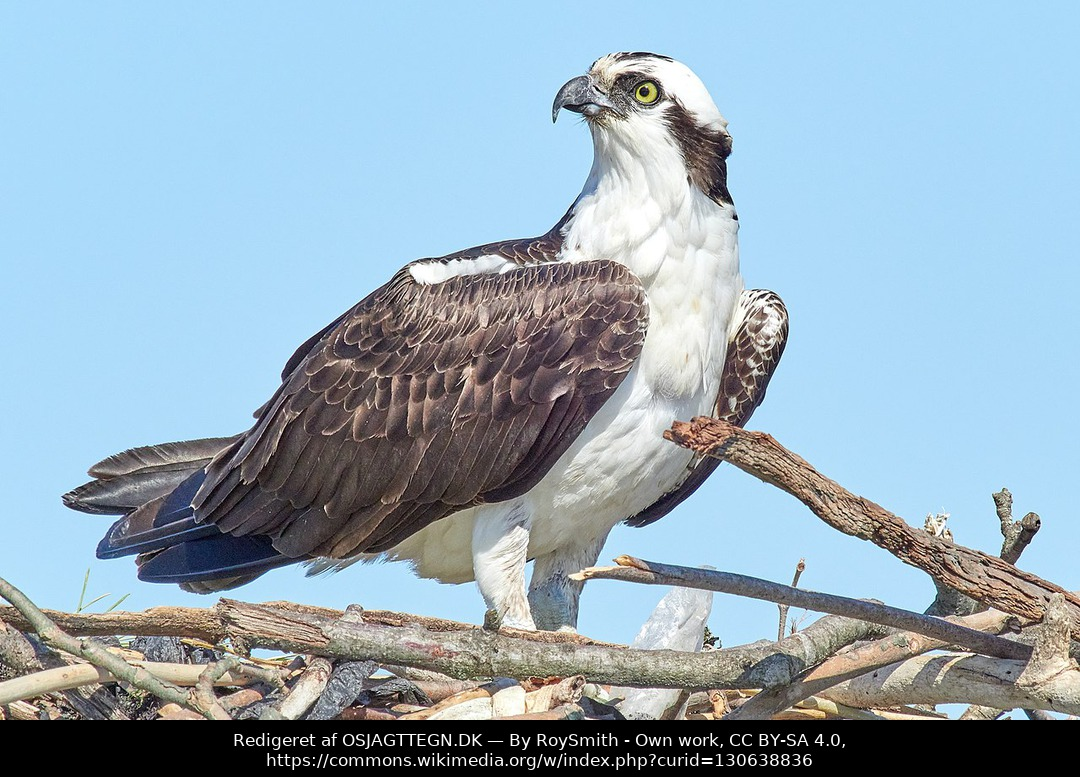
\includegraphics[width=\linewidth, height=7.2cm, keepaspectratio]{Billeder/Dyr/Fugle/Rovfugle/fiskeørn.jpg}
  \end{columns}
\end{frame}
\begin{frame}
  \vspace{3em}
  \begin{center}
    {\LARGE \textbf{Vadefugle}}
  \end{center}
\end{frame}

\section{Vadefugle (vildtkending og biologi)}

\begin{frame}{%
\begin{minipage}[t]{0.85\textwidth}
Strandskade
\end{minipage}%
\hfill
\begin{minipage}[t]{0.1\textwidth}
\raggedleft

\includegraphics[width=0.55cm, height=0.55cm, keepaspectratio]{Billeder/Ikoner/star.png}%
\end{minipage}%
}
\vspace{0.25em}
\begin{columns}[T]
% --- Venstre kolonne: Tekst ---
\column{0.55\textwidth}
\setlength{\parskip}{0.5em}
\small
\RaggedRight\textbf{\textit{Haematopus ostralegus}} – karakteristisk sort hvid vadefugl\par

\textbf{Udseende:} \\
\quad –  Sort/hvid fjerdragt, røde øjne, langt rødt næb og røde ben.  

% --- Højre kolonne: Et billede ---
\column{0.40\textwidth}
\centering
\fbox{%
\begin{minipage}{\linewidth}
\centering
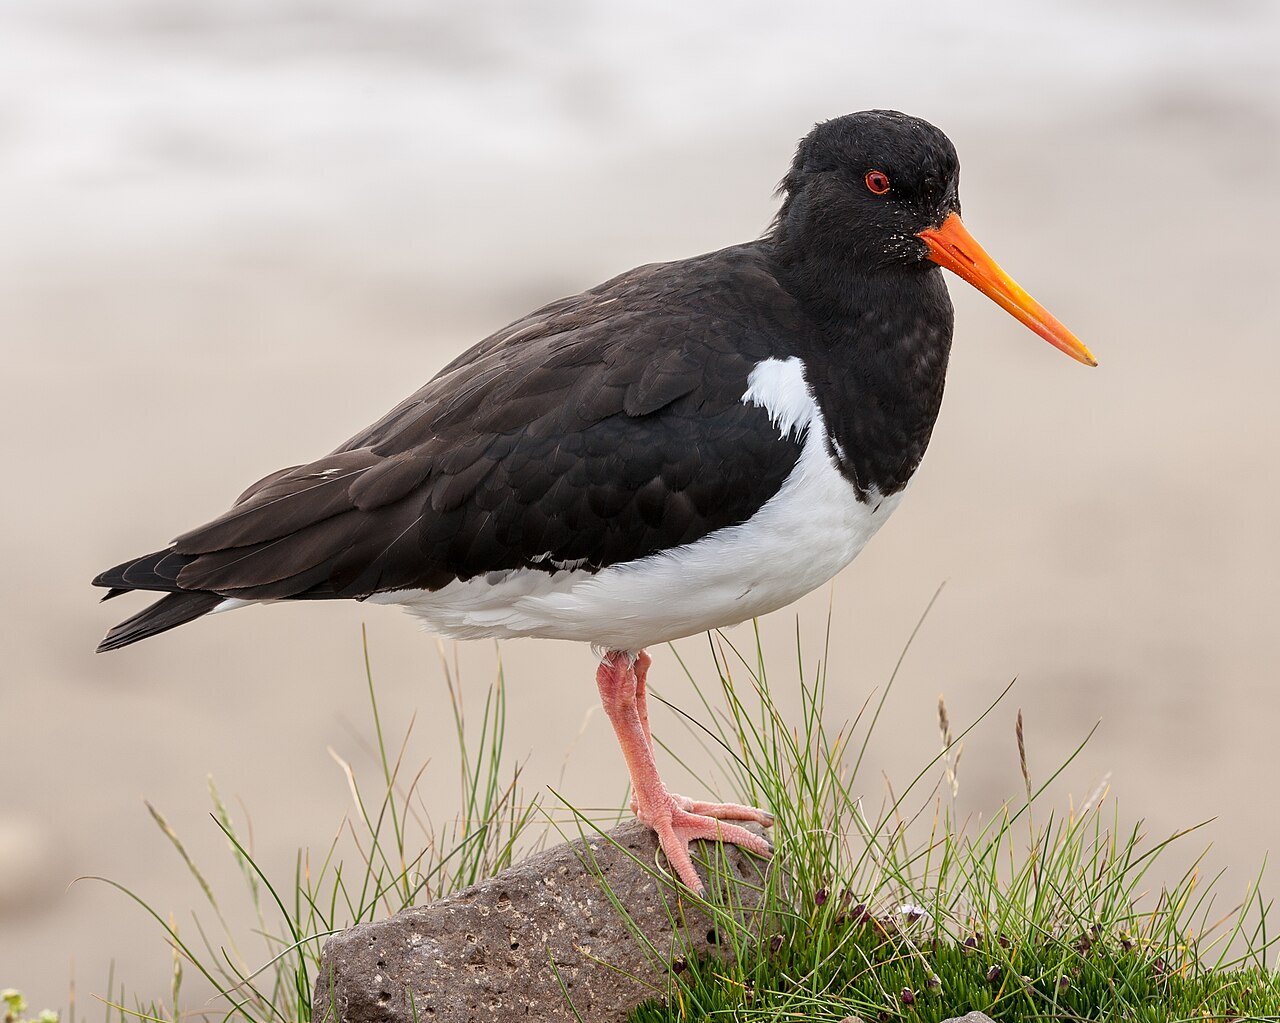
\includegraphics[width=0.8\linewidth, height=10cm, keepaspectratio]{Billeder/Dyr/Fugle/Vadefugle/strandskade.jpg}
\end{minipage}
}%
\end{columns}
\end{frame}
\begin{frame}{%
\begin{minipage}[t]{0.85\textwidth}
Vibe
\end{minipage}%
\hfill
\begin{minipage}[t]{0.1\textwidth}
\raggedleft

\includegraphics[width=0.55cm, height=0.55cm, keepaspectratio]{Billeder/Ikoner/star.png}%
\end{minipage}%
}
\vspace{0.25em}
\begin{columns}[T]
% --- Venstre kolonne: Tekst ---
\column{0.55\textwidth}
\setlength{\parskip}{0.5em}
\small
\RaggedRight\textbf{\textit{Vanellus vanellus}} – karakteristisk med fjertoppen på hvoedet\par

\textbf{Udseende:} \\
\quad –  Metalgrøn ryg, hvid bug, sort bryst og pande. Lang nakketop på hovedet.   

% --- Højre kolonne: Et billede ---
\column{0.40\textwidth}
\centering
\fbox{%
\begin{minipage}{\linewidth}
\centering
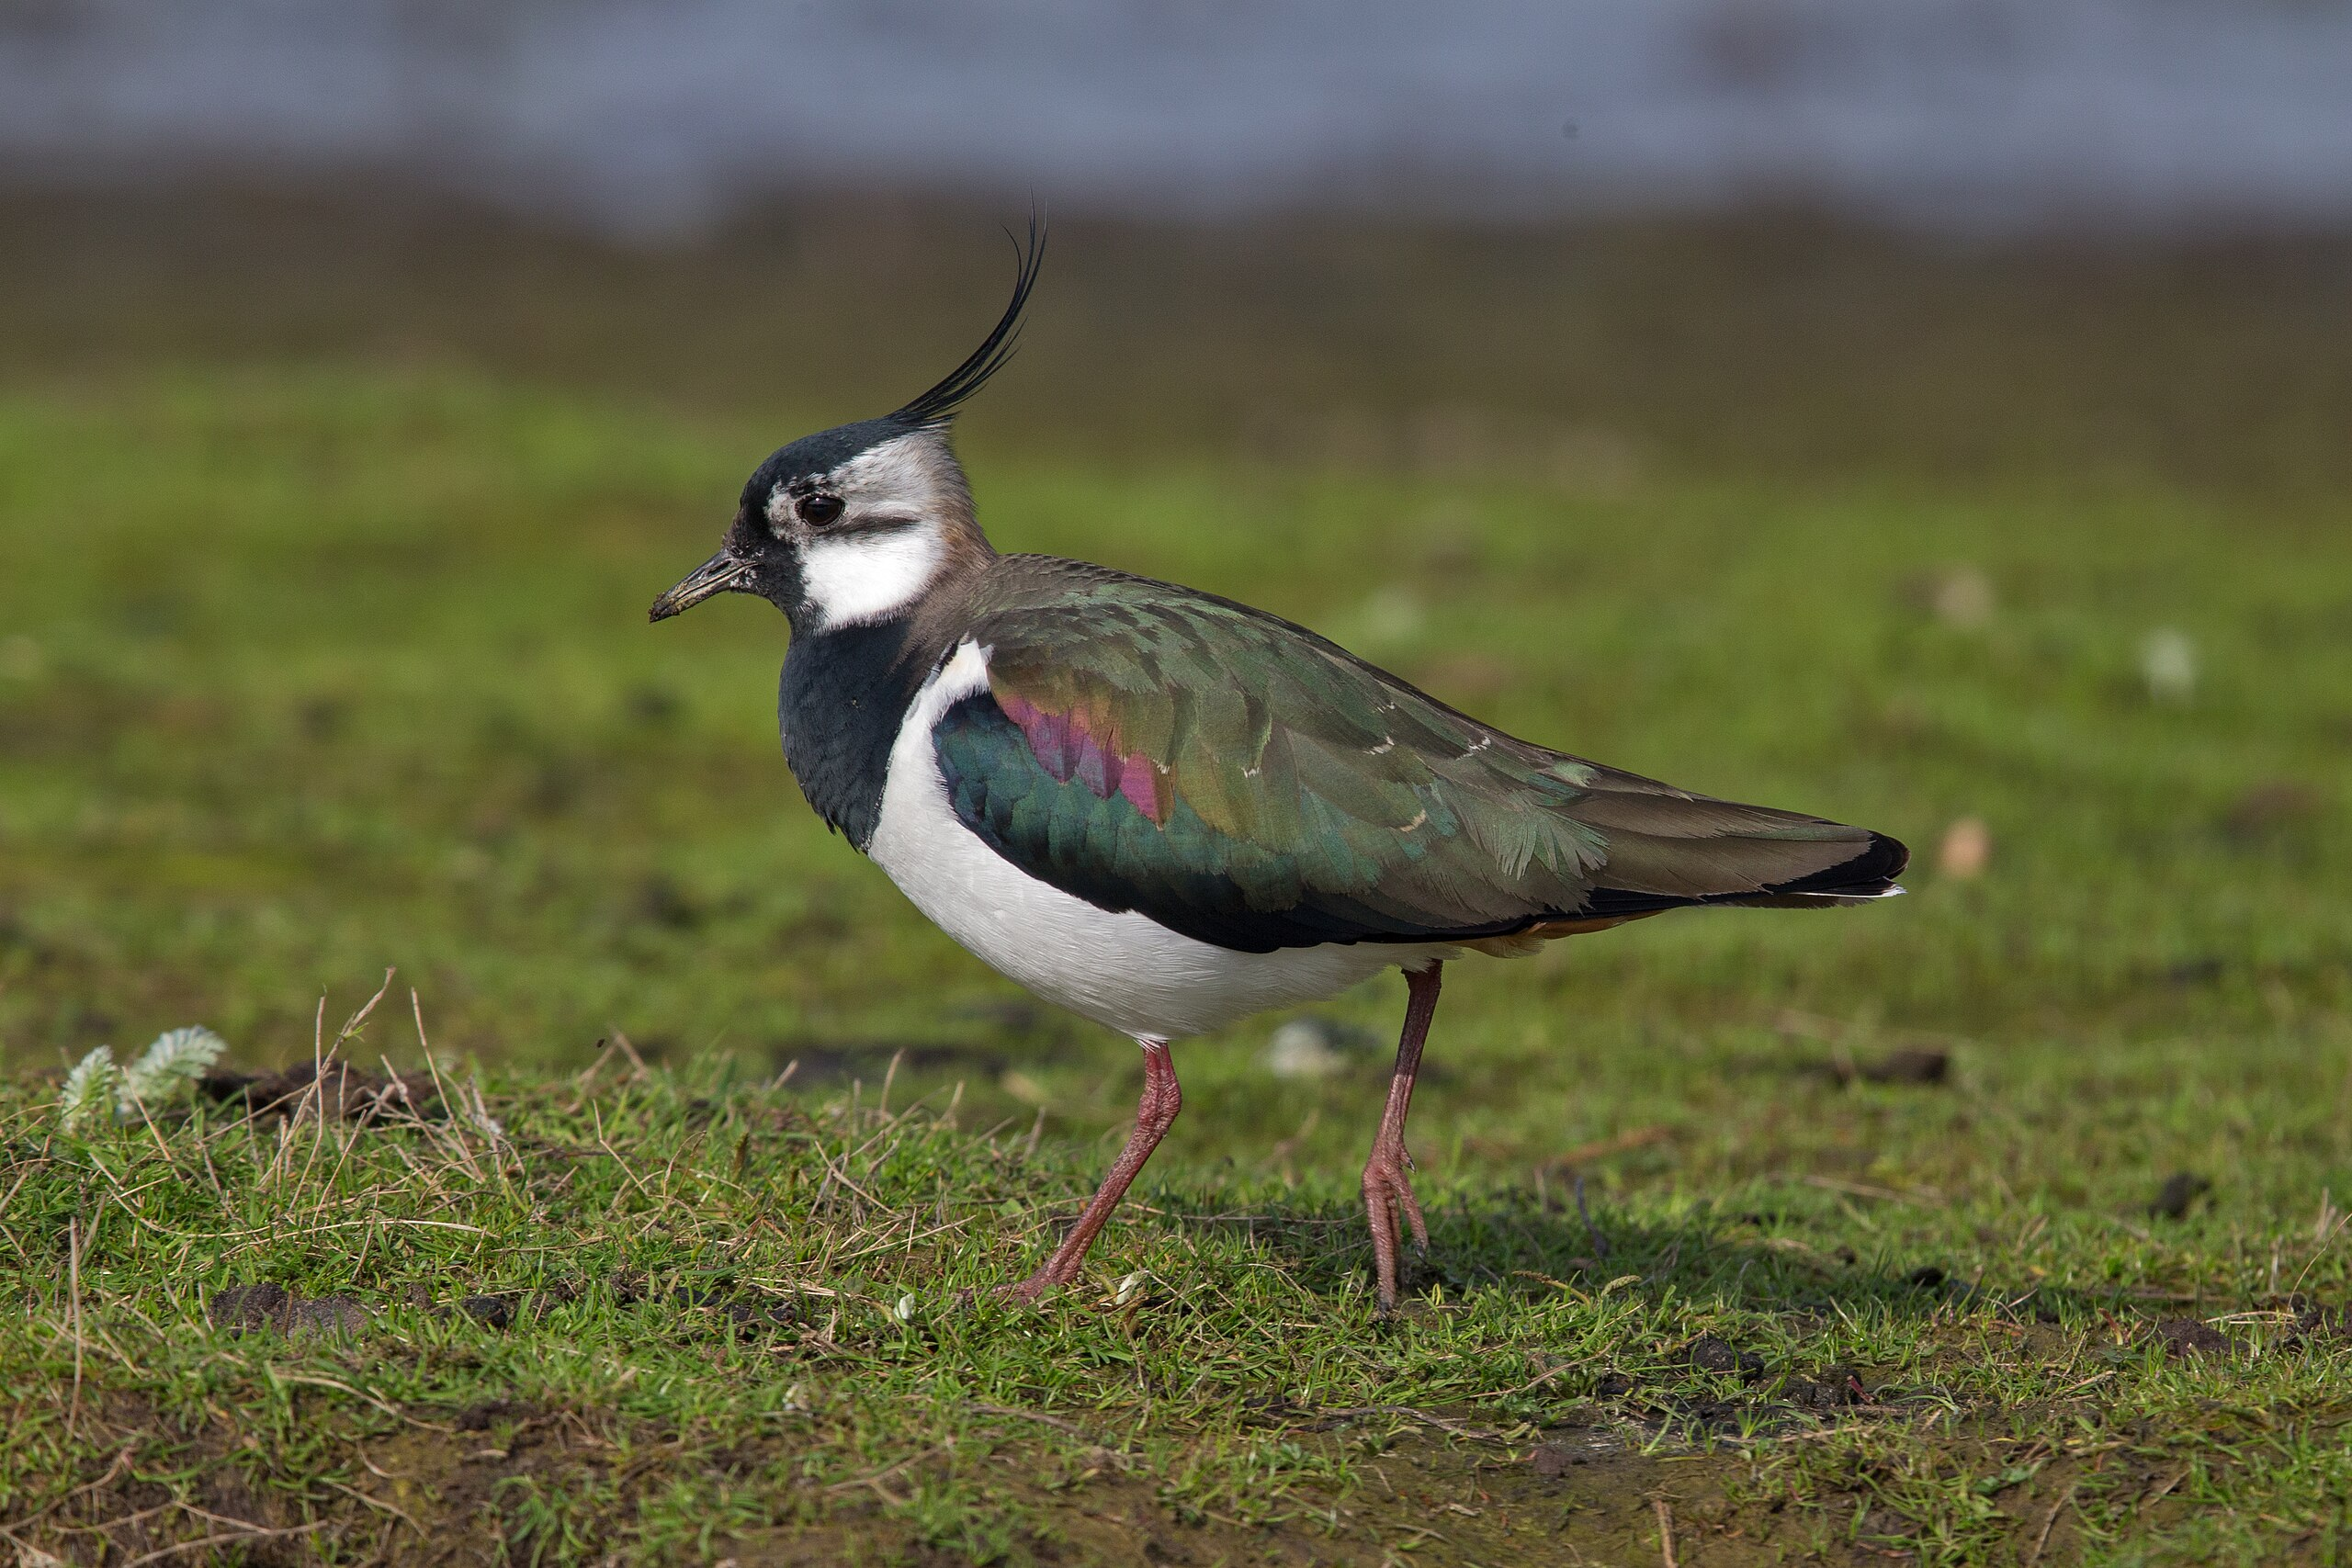
\includegraphics[width=0.8\linewidth, height=10cm, keepaspectratio]{Billeder/Dyr/Fugle/Vadefugle/vibe.jpg}
\end{minipage}
}%
\end{columns}
\end{frame}
\begin{frame}{%
\begin{minipage}[t]{0.85\textwidth}
Hjejle
\end{minipage}%
\hfill
\begin{minipage}[t]{0.1\textwidth}
\raggedleft

\includegraphics[width=0.5cm, height=0.5cm, keepaspectratio]{Billeder/Ikoner/star.png}%
\hspace{0.2em}%

\includegraphics[width=0.5cm, height=0.5cm, keepaspectratio]{Billeder/Ikoner/star.png}
\end{minipage}%
}
\vspace{0.25em}
\begin{columns}[T]
% --- Venstre kolonne: Tekst ---
\column{0.55\textwidth}
\setlength{\parskip}{0.5em}
\small
\RaggedRight\textbf{\textit{Pluvialis apricaria}} – Mellemstor vadefugl som kan forveksles med strandhjejle\par 

\textbf{Udseende:} \\
\quad – Buttet krop, store øjne, rundt hoved og kort næb. Spraglet ryg med sort, grøn og hvide nuancer.  \par

\textbf{Levesteder:} \\
\quad – Marker og enge, primært Vestjylland

\textbf{Føde:} \\
\quad – Primært animals: orme, insekter, snegle  \par

\textbf{Udbredelse:} \\
\quad – Sjælden ynglefugl. Ses primært som trækfugl \par

\textbf{Træk/standfugl} \\
\quad – Trækfugl \par

% --- Højre kolonne: Kun ét billede (Hannen) ---
\column{0.40\textwidth}
\centering
\fbox{%
\begin{minipage}{\linewidth}
\centering
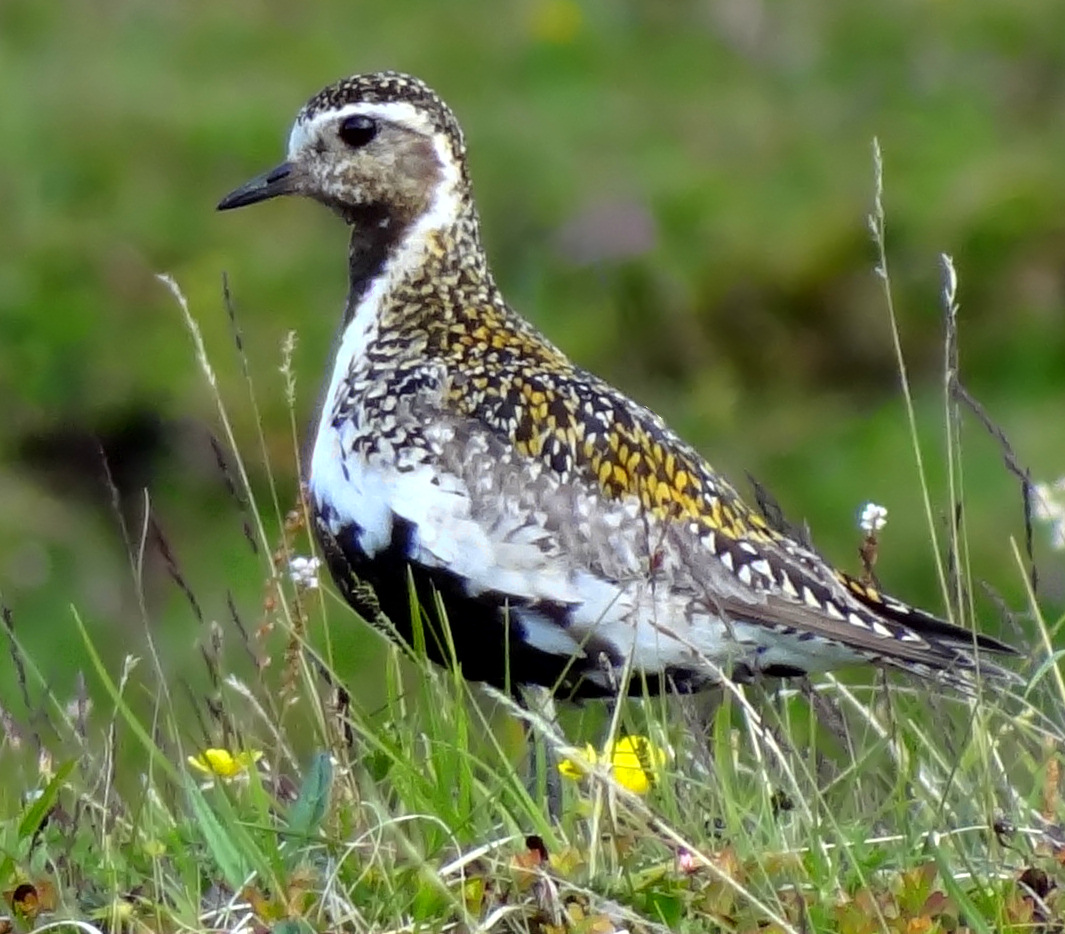
\includegraphics[width=0.8\linewidth, height=6.5cm, keepaspectratio]{Billeder/Dyr/Fugle/Vadefugle/hjejle.jpg}%
\end{minipage}
}%
\end{columns}
\end{frame}
\begin{frame}{%
\begin{minipage}[t]{0.85\textwidth}
Strandhjejle
\end{minipage}%
\hfill
\begin{minipage}[t]{0.1\textwidth}
\raggedleft

\includegraphics[width=0.55cm, height=0.55cm, keepaspectratio]{Billeder/Ikoner/star.png}%
\end{minipage}%
}
\vspace{0.25em}
\begin{columns}[T]
% --- Venstre kolonne: Tekst ---
\column{0.55\textwidth}
\setlength{\parskip}{0.5em}
\small
\RaggedRight\textbf{\textit{Pluvialis squatarola}} – Ligner hjeljlen men har hvid isse\par

\textbf{Udseende:} \\
\quad –  Sort hvid ryg som adskiller den fra hjejlen same den hvide isse  

% --- Højre kolonne: Et billede ---
\column{0.40\textwidth}
\centering
\fbox{%
\begin{minipage}{\linewidth}
\centering
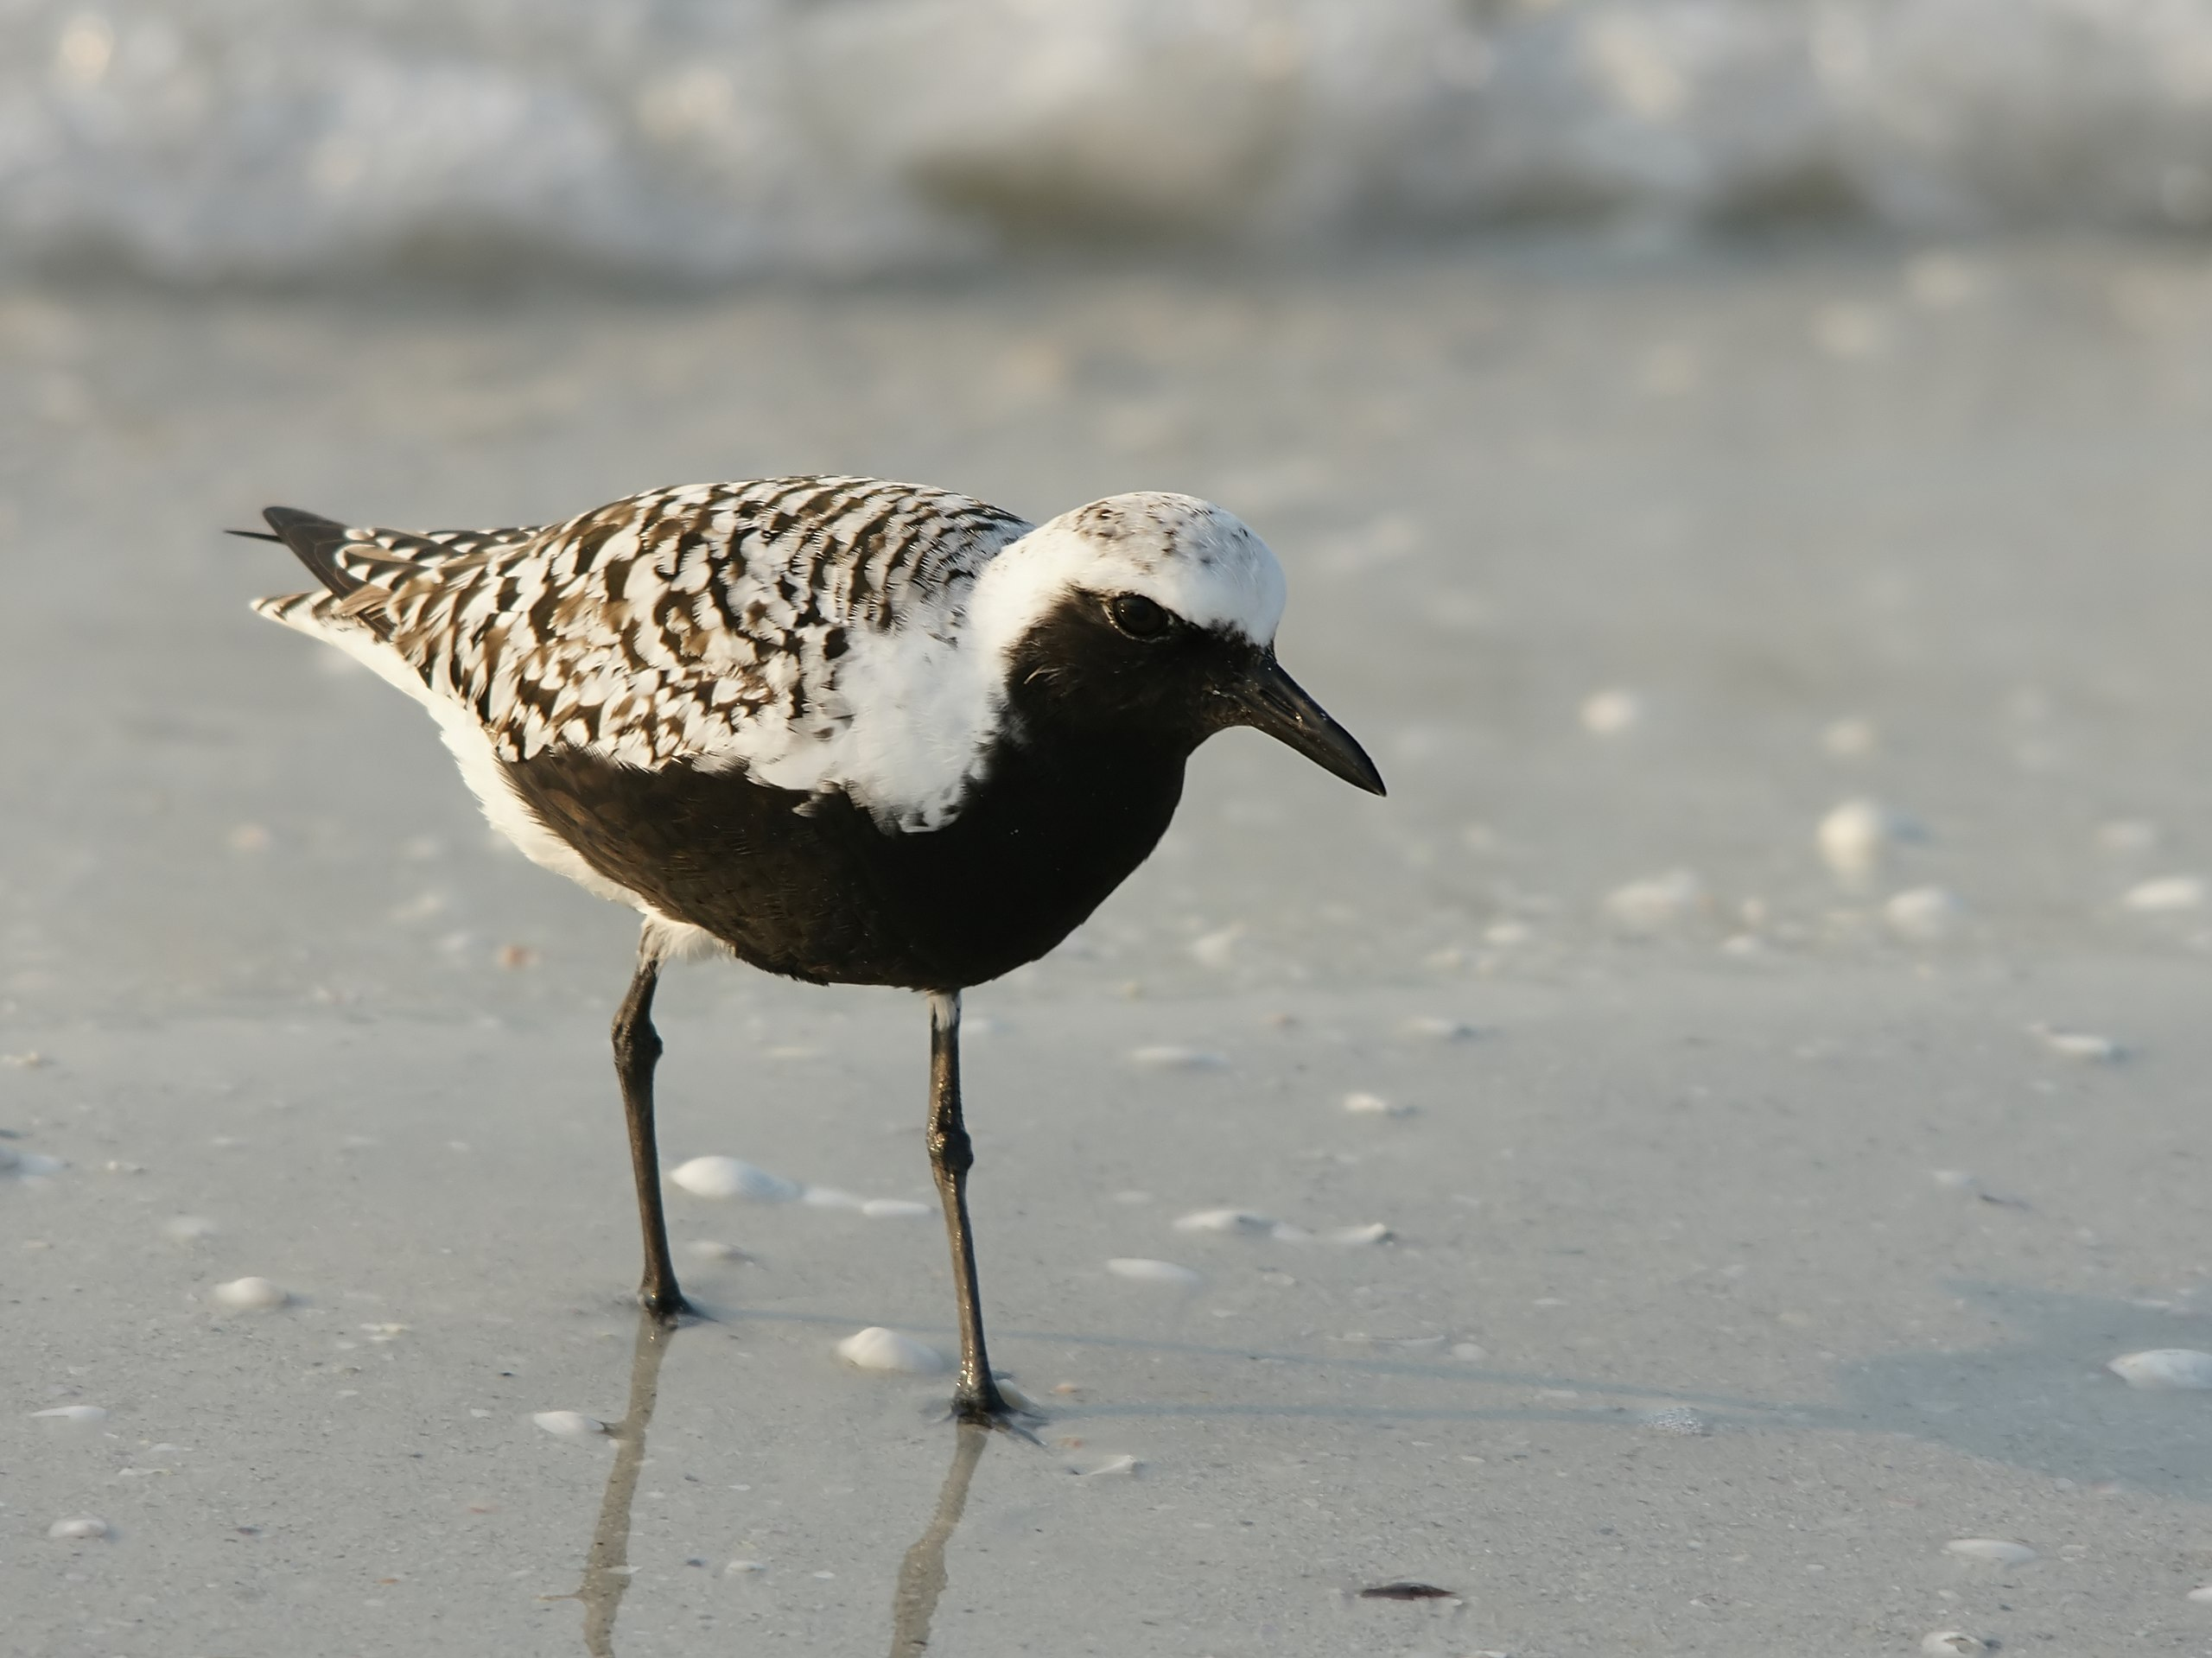
\includegraphics[width=0.8\linewidth, height=10cm, keepaspectratio]{Billeder/Dyr/Fugle/Vadefugle/strandhjejle.jpg}
\end{minipage}
}%
\end{columns}
\end{frame}
\begin{frame}{%
\begin{minipage}[t]{0.85\textwidth}
Stor regnspove
\end{minipage}%
\hfill
\begin{minipage}[t]{0.1\textwidth}
\raggedleft

\includegraphics[width=0.5cm, height=0.5cm, keepaspectratio]{Billeder/Ikoner/star.png}%
\hspace{0.2em}%

\includegraphics[width=0.5cm, height=0.5cm, keepaspectratio]{Billeder/Ikoner/star.png}
\end{minipage}%
}
\vspace{0.25em}
\begin{columns}[T]
% --- Venstre kolonne: Tekst ---
\column{0.55\textwidth}
\setlength{\parskip}{0.5em}
\small
\RaggedRight\textbf{\textit{Numenius arquata}} – Kendes på det lange nedadbøjet næb isse\par 

\textbf{Udseende:} \\
\quad – Kroppen er gråbrun med længdestriber. Næbbet er meget langt og nedadbøjet. Lange ben.  \par

\textbf{Levesteder:} \\
\quad – Kyster, lavvandede søer, enge og heder

\textbf{Føde:} \\
\quad – Børste- og sandorm, snegle, regnorm, insektlarver, krebsydr muslinger og bær \par

\textbf{Udbredelse:} \\
\quad – Primært Jylland \par

\textbf{Træk/standfugl} \\
\quad – Få yngler, alm trækfugl \par

% --- Højre kolonne: Kun ét billede (Hannen) ---
\column{0.40\textwidth}
\centering
\fbox{%
\begin{minipage}{\linewidth}
\centering
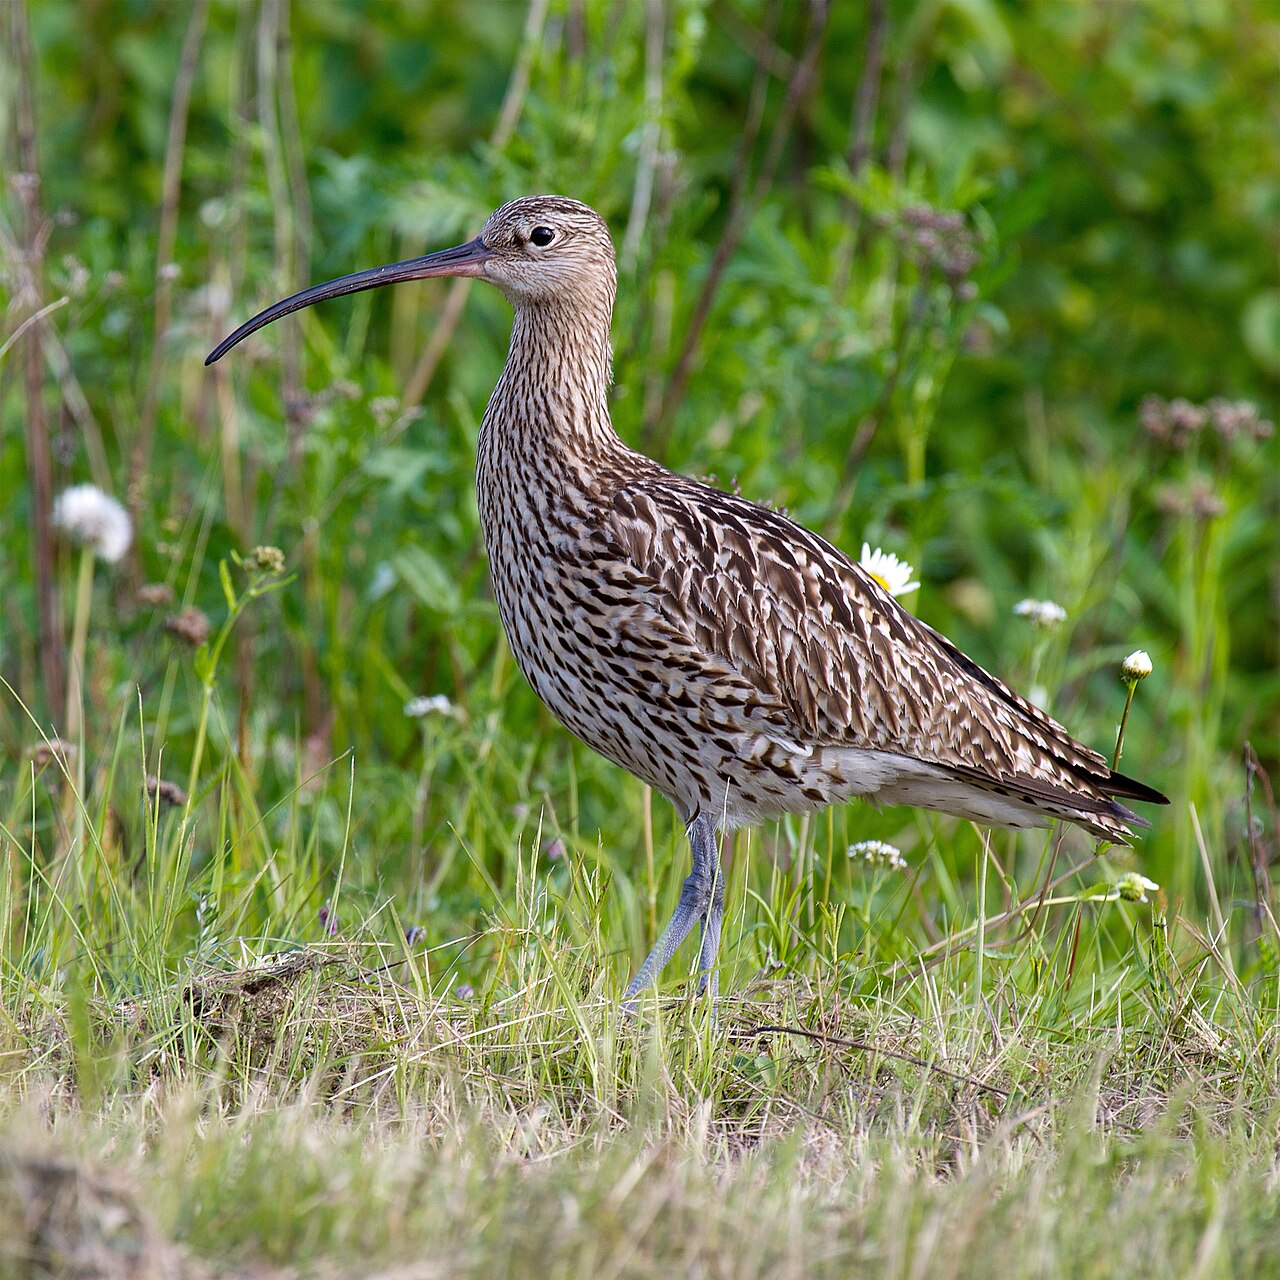
\includegraphics[width=0.8\linewidth, height=6.5cm, keepaspectratio]{Billeder/Dyr/Fugle/Vadefugle/stor_regnspove.jpg}%
\end{minipage}
}%
\end{columns}
\end{frame}
\begin{frame}{%
\begin{minipage}[t]{0.85\textwidth}
Lille regnspove
\end{minipage}%
\hfill
\begin{minipage}[t]{0.1\textwidth}
\raggedleft

\includegraphics[width=0.55cm, height=0.55cm, keepaspectratio]{Billeder/Ikoner/star.png}%
\end{minipage}%
}
\vspace{0.25em}
\begin{columns}[T]
% --- Venstre kolonne: Tekst ---
\column{0.55\textwidth}
\setlength{\parskip}{0.5em}
\small
\RaggedRight\textbf{\textit{Numenius phaeopus}} – også kaldet Småspove, langt nedadbøjet næb \par

\textbf{Udseende:} \\
\quad –  Mørk øjenstribe og tydelige brune issestriber med hvid midterskilning. Langt nedadbøjet næb.  

% --- Højre kolonne: Et billede ---
\column{0.40\textwidth}
\centering
\fbox{%
\begin{minipage}{\linewidth}
\centering
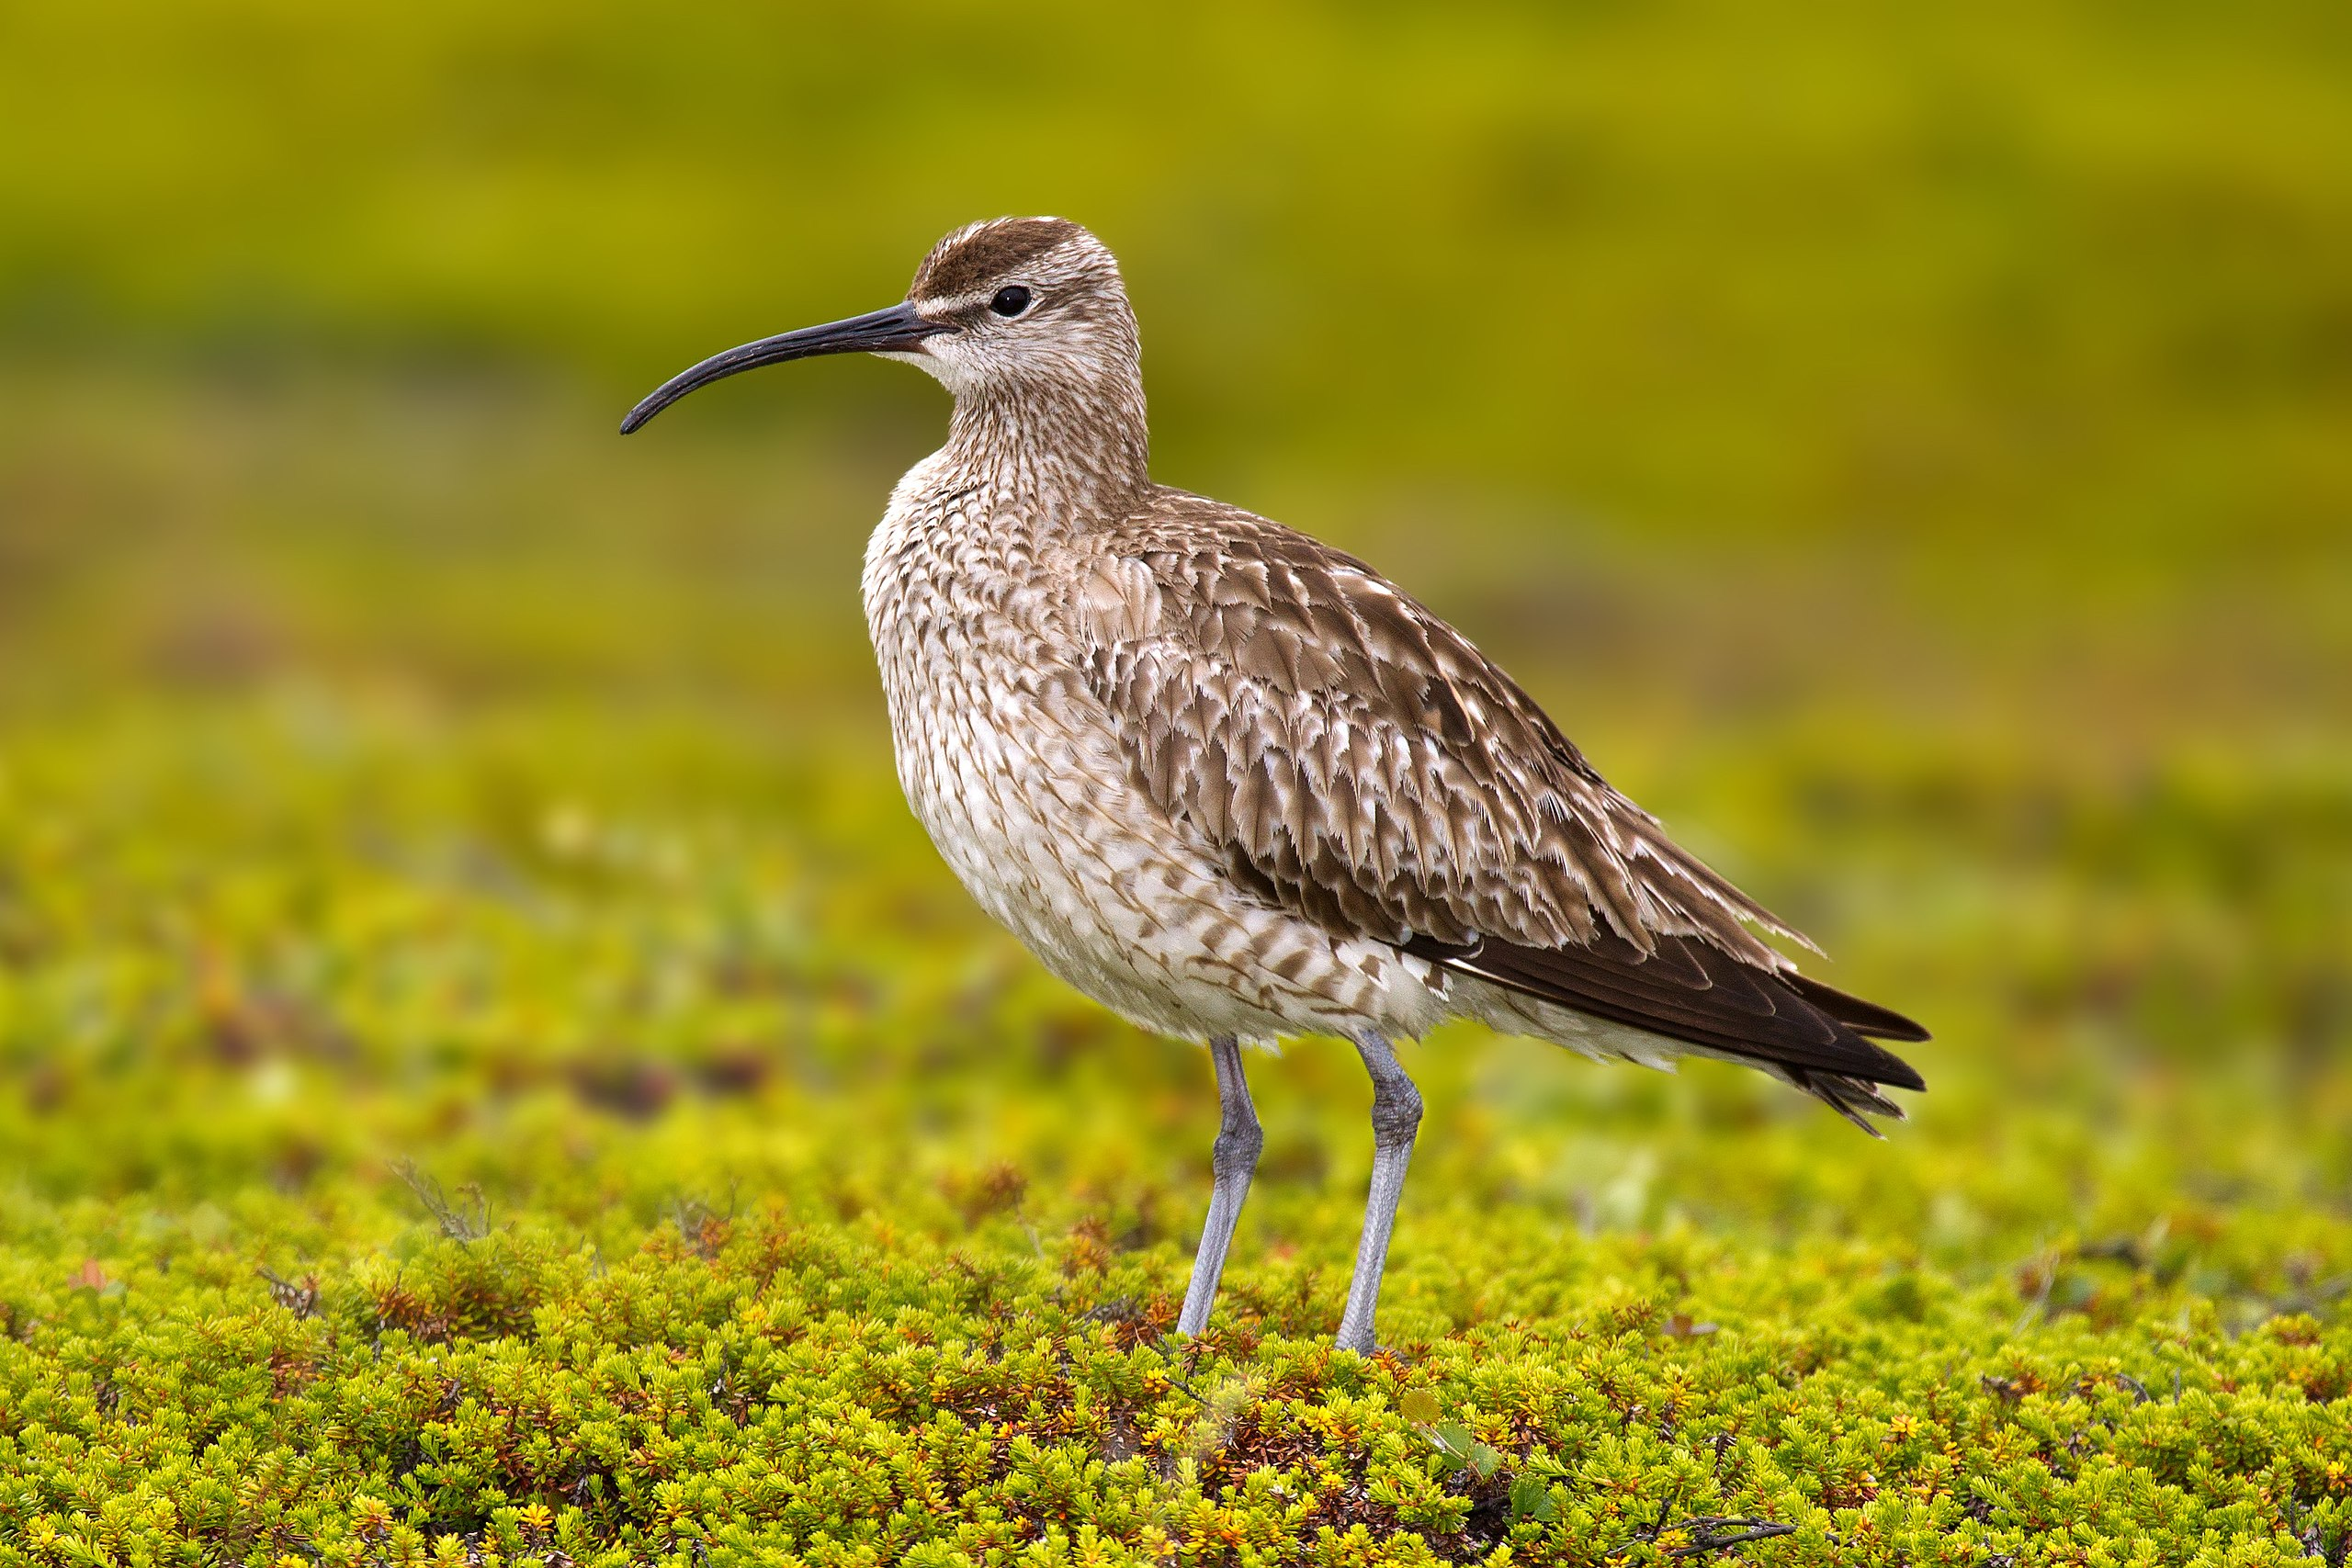
\includegraphics[width=0.8\linewidth, height=10cm, keepaspectratio]{Billeder/Dyr/Fugle/Vadefugle/lille_regnspove.jpg}
\end{minipage}
}%
\end{columns}
\end{frame}



\begin{frame}{%
  \begin{minipage}[t]{0.85\textwidth}
    Lille kobbersneppe
  \end{minipage}%
  \hfill
  \begin{minipage}[t]{0.1\textwidth}
    \raggedleft
    
\includegraphics[width=0.55cm, height=0.55cm, keepaspectratio]{Billeder/Ikoner/star.png}%
  \end{minipage}%
} 
  \vspace{0.25em}
  \begin{columns}[T]
    % --- Venstre kolonne: Tekst ---
    \column{0.55\textwidth}
    \setlength{\parskip}{0.5em}
    \small
    \RaggedRight\textbf{\textit{Limosa lapponica}} – langt næb og lange ben \par

    \textbf{Udseende:} \\
    \quad – Kobberfarvet. Langt let opadbuet næb. Lysere ved næbroden \par

    

    % --- Højre kolonne: To billeder stablet over hinanden ---
    \column{0.40\textwidth}
    \centering
    \fbox{%
      \begin{minipage}{\linewidth}
        \centering
        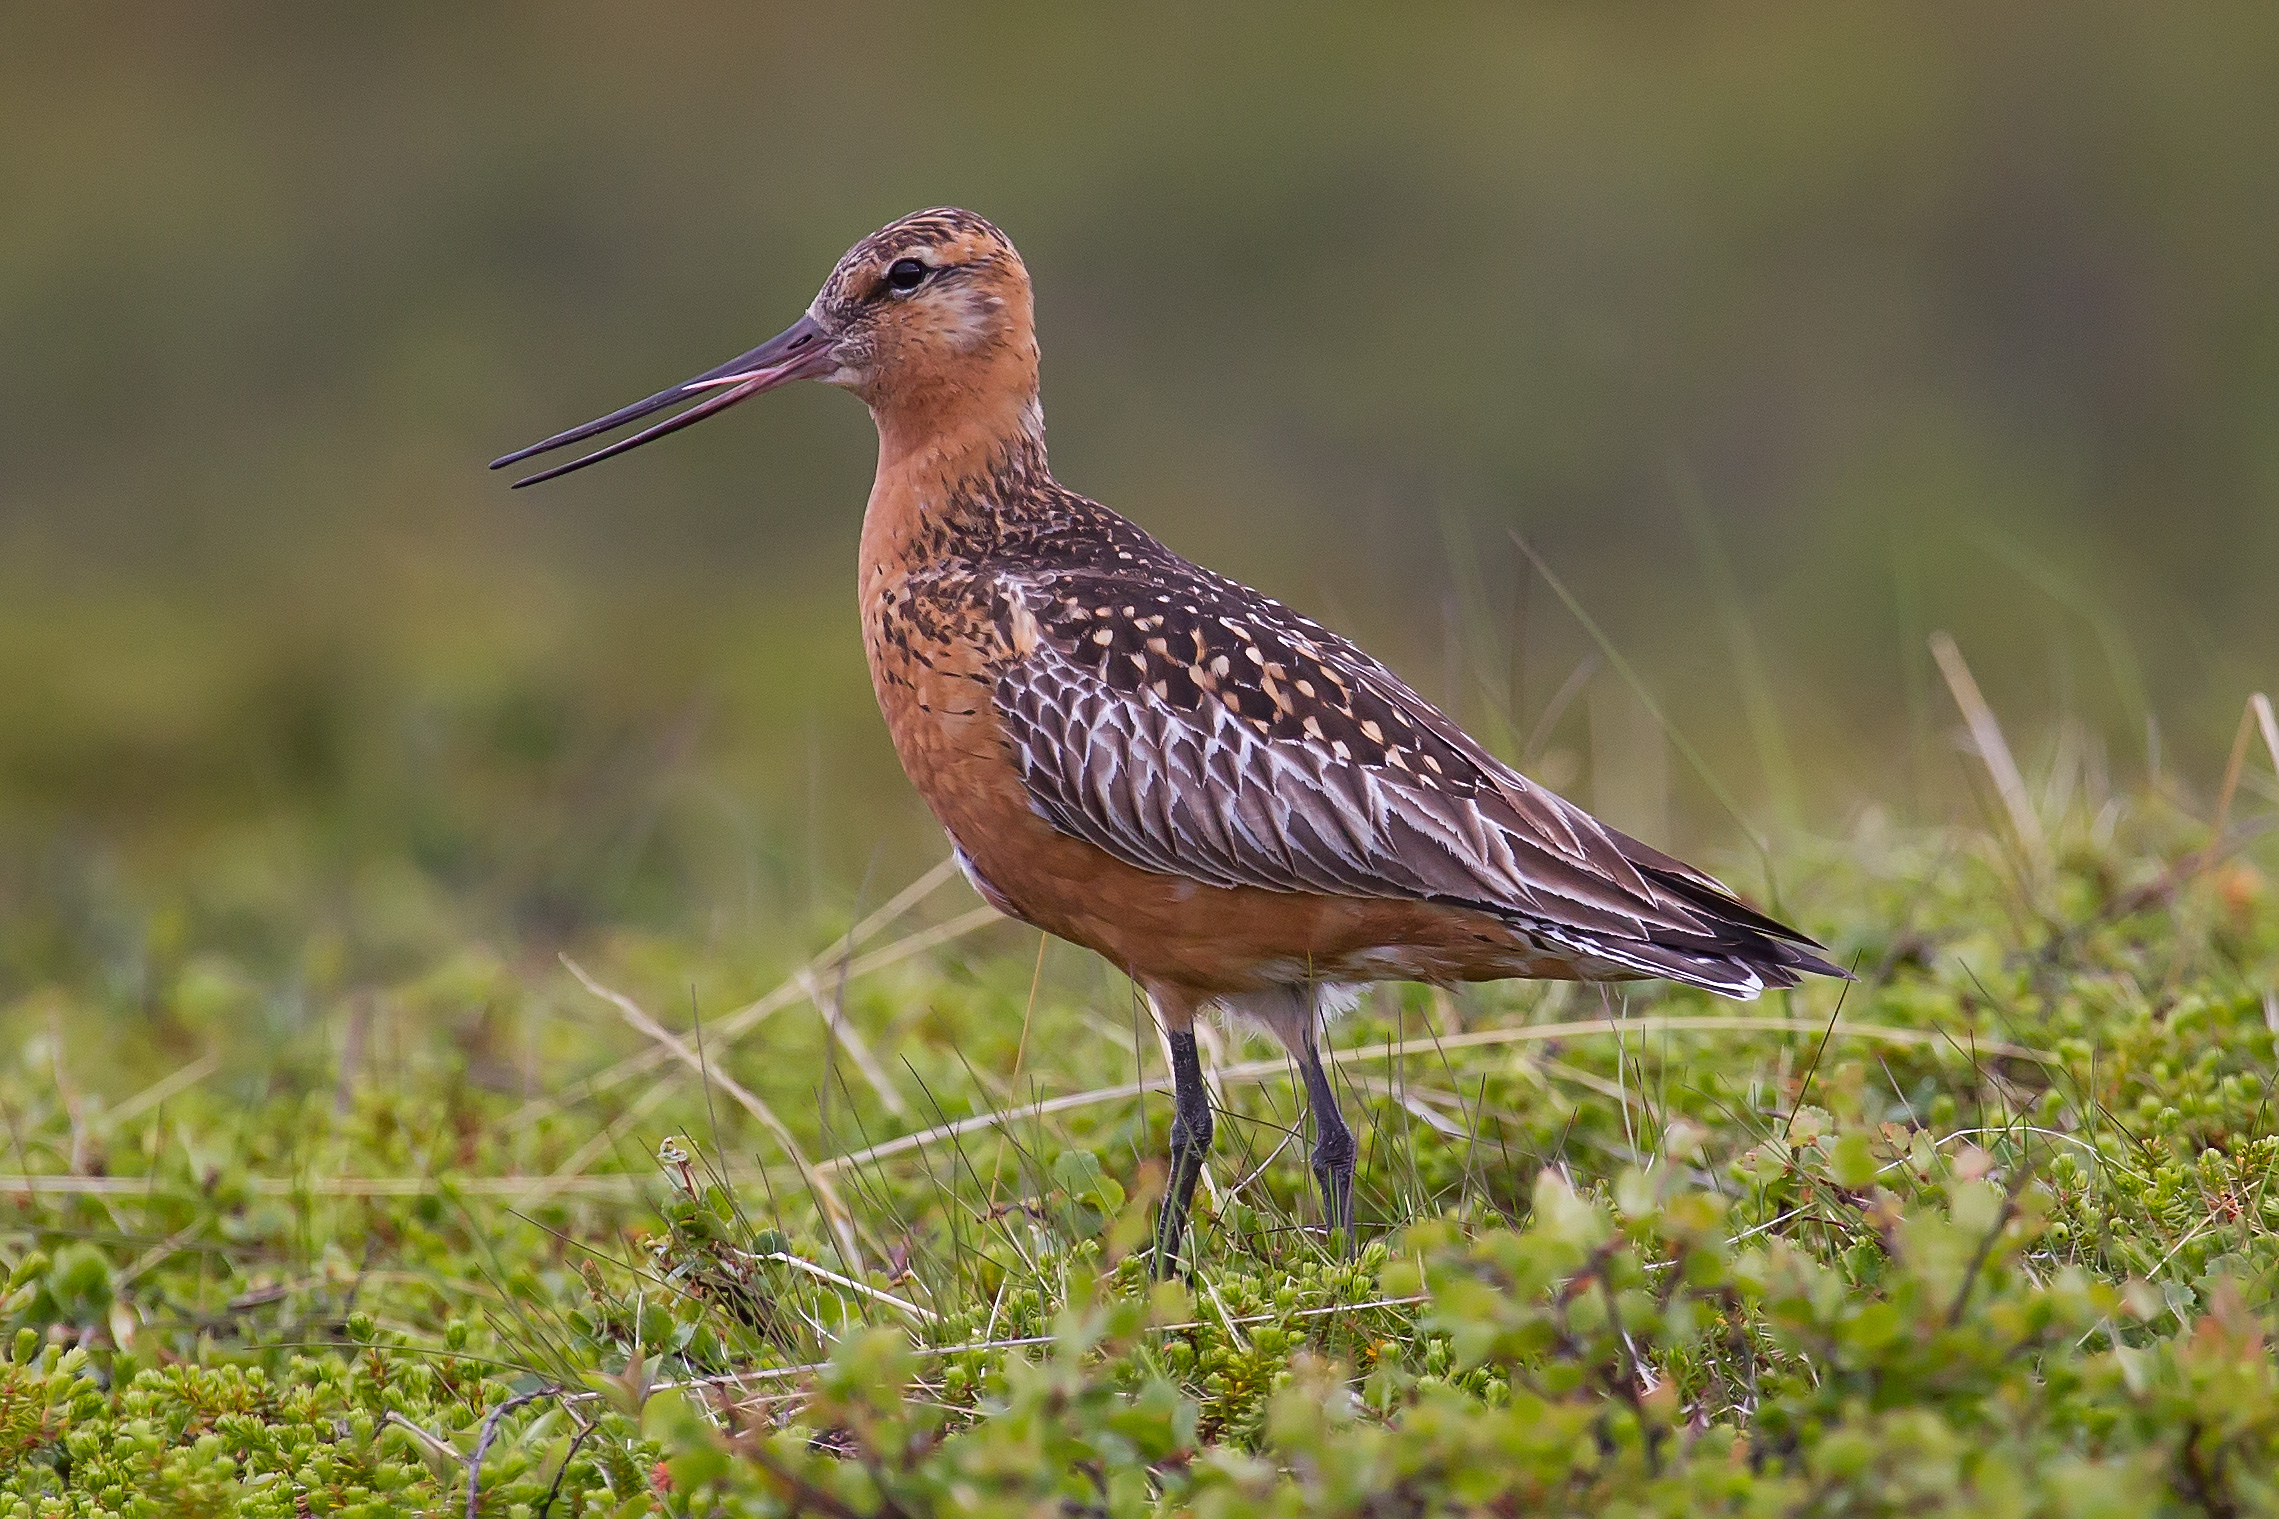
\includegraphics[width=0.8\linewidth, height=3cm, keepaspectratio]{Billeder/Dyr/Fugle/Vadefugle/lille_kobbersneppe_sommer.jpg}\\[0.5em]
        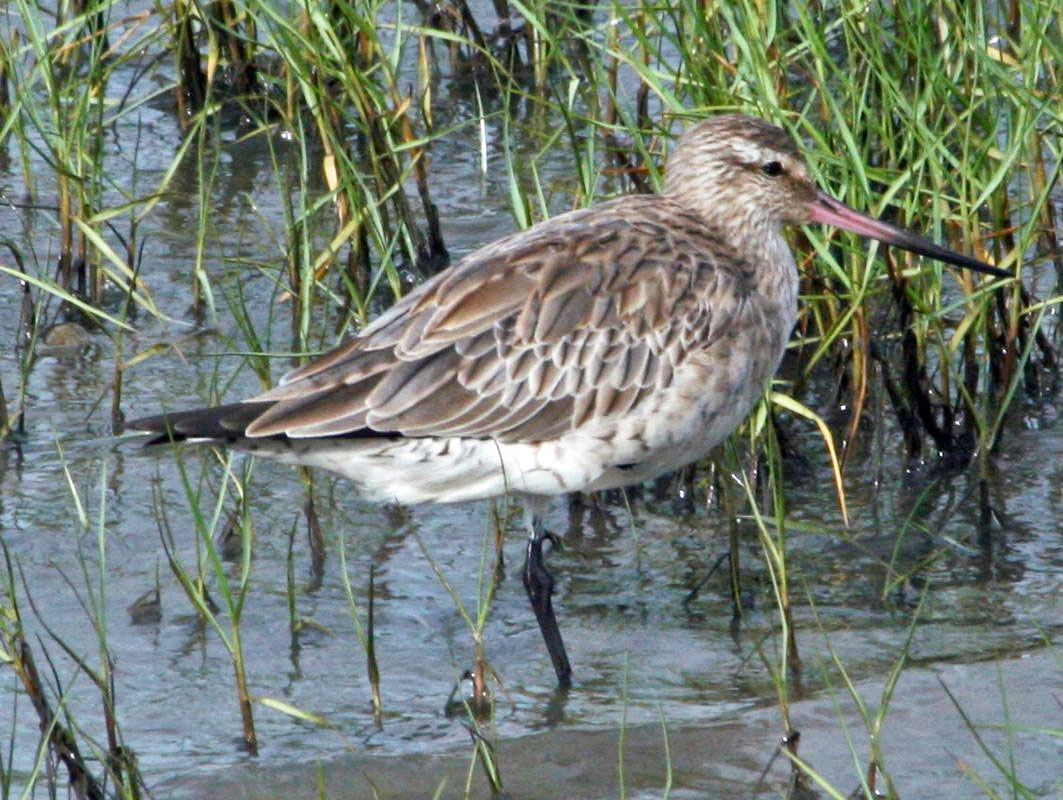
\includegraphics[width=0.8\linewidth, height=3cm, keepaspectratio]{Billeder/Dyr/Fugle/Vadefugle/lille_kobbersneppe_vinter.jpg}%
      \end{minipage}
    }%
    \vspace{0.05em}
    \footnotesize Sommerdragt øverst, vinter nederst
  \end{columns}
\end{frame}
\begin{frame}{%
\begin{minipage}[t]{0.85\textwidth}
Stor kobbersneppe
\end{minipage}%
\hfill
\begin{minipage}[t]{0.1\textwidth}
\raggedleft

\includegraphics[width=0.55cm, height=0.55cm, keepaspectratio]{Billeder/Ikoner/star.png}%
\end{minipage}%
}
\vspace{0.25em}
\begin{columns}[T]
% --- Venstre kolonne: Tekst ---
\column{0.55\textwidth}
\setlength{\parskip}{0.5em}
\small
\RaggedRight\textbf{\textit{Limosa limosa}} – stor slank vadefugl med langt næb\par

\textbf{Udseende:} \\
\quad –  Lange ben og langt svagt opadbuet næb. Næbbet er orangegult med sort spids.   

% --- Højre kolonne: Et billede ---
\column{0.40\textwidth}
\centering
\fbox{%
\begin{minipage}{\linewidth}
\centering
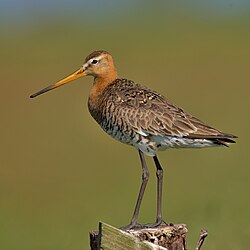
\includegraphics[width=0.8\linewidth, height=10cm, keepaspectratio]{Billeder/Dyr/Fugle/Vadefugle/stor_kobbersneppe.jpg}
\end{minipage}
}%
\end{columns}
\end{frame}
\begin{frame}{%
\begin{minipage}[t]{0.85\textwidth}
Rødben
\end{minipage}%
\hfill
\begin{minipage}[t]{0.1\textwidth}
\raggedleft

\includegraphics[width=0.55cm, height=0.55cm, keepaspectratio]{Billeder/Ikoner/star.png}%
\end{minipage}%
}
\vspace{0.25em}
\begin{columns}[T]
% --- Venstre kolonne: Tekst ---
\column{0.55\textwidth}
\setlength{\parskip}{0.5em}
\small
\RaggedRight\textbf{\textit{Tringa totanus}} – Lys vadefugl med røde ben\par

\textbf{Udseende:} \\
\quad –  Røde ben, rød næb med sort spids.  

% --- Højre kolonne: Et billede ---
\column{0.40\textwidth}
\centering
\fbox{%
\begin{minipage}{\linewidth}
\centering
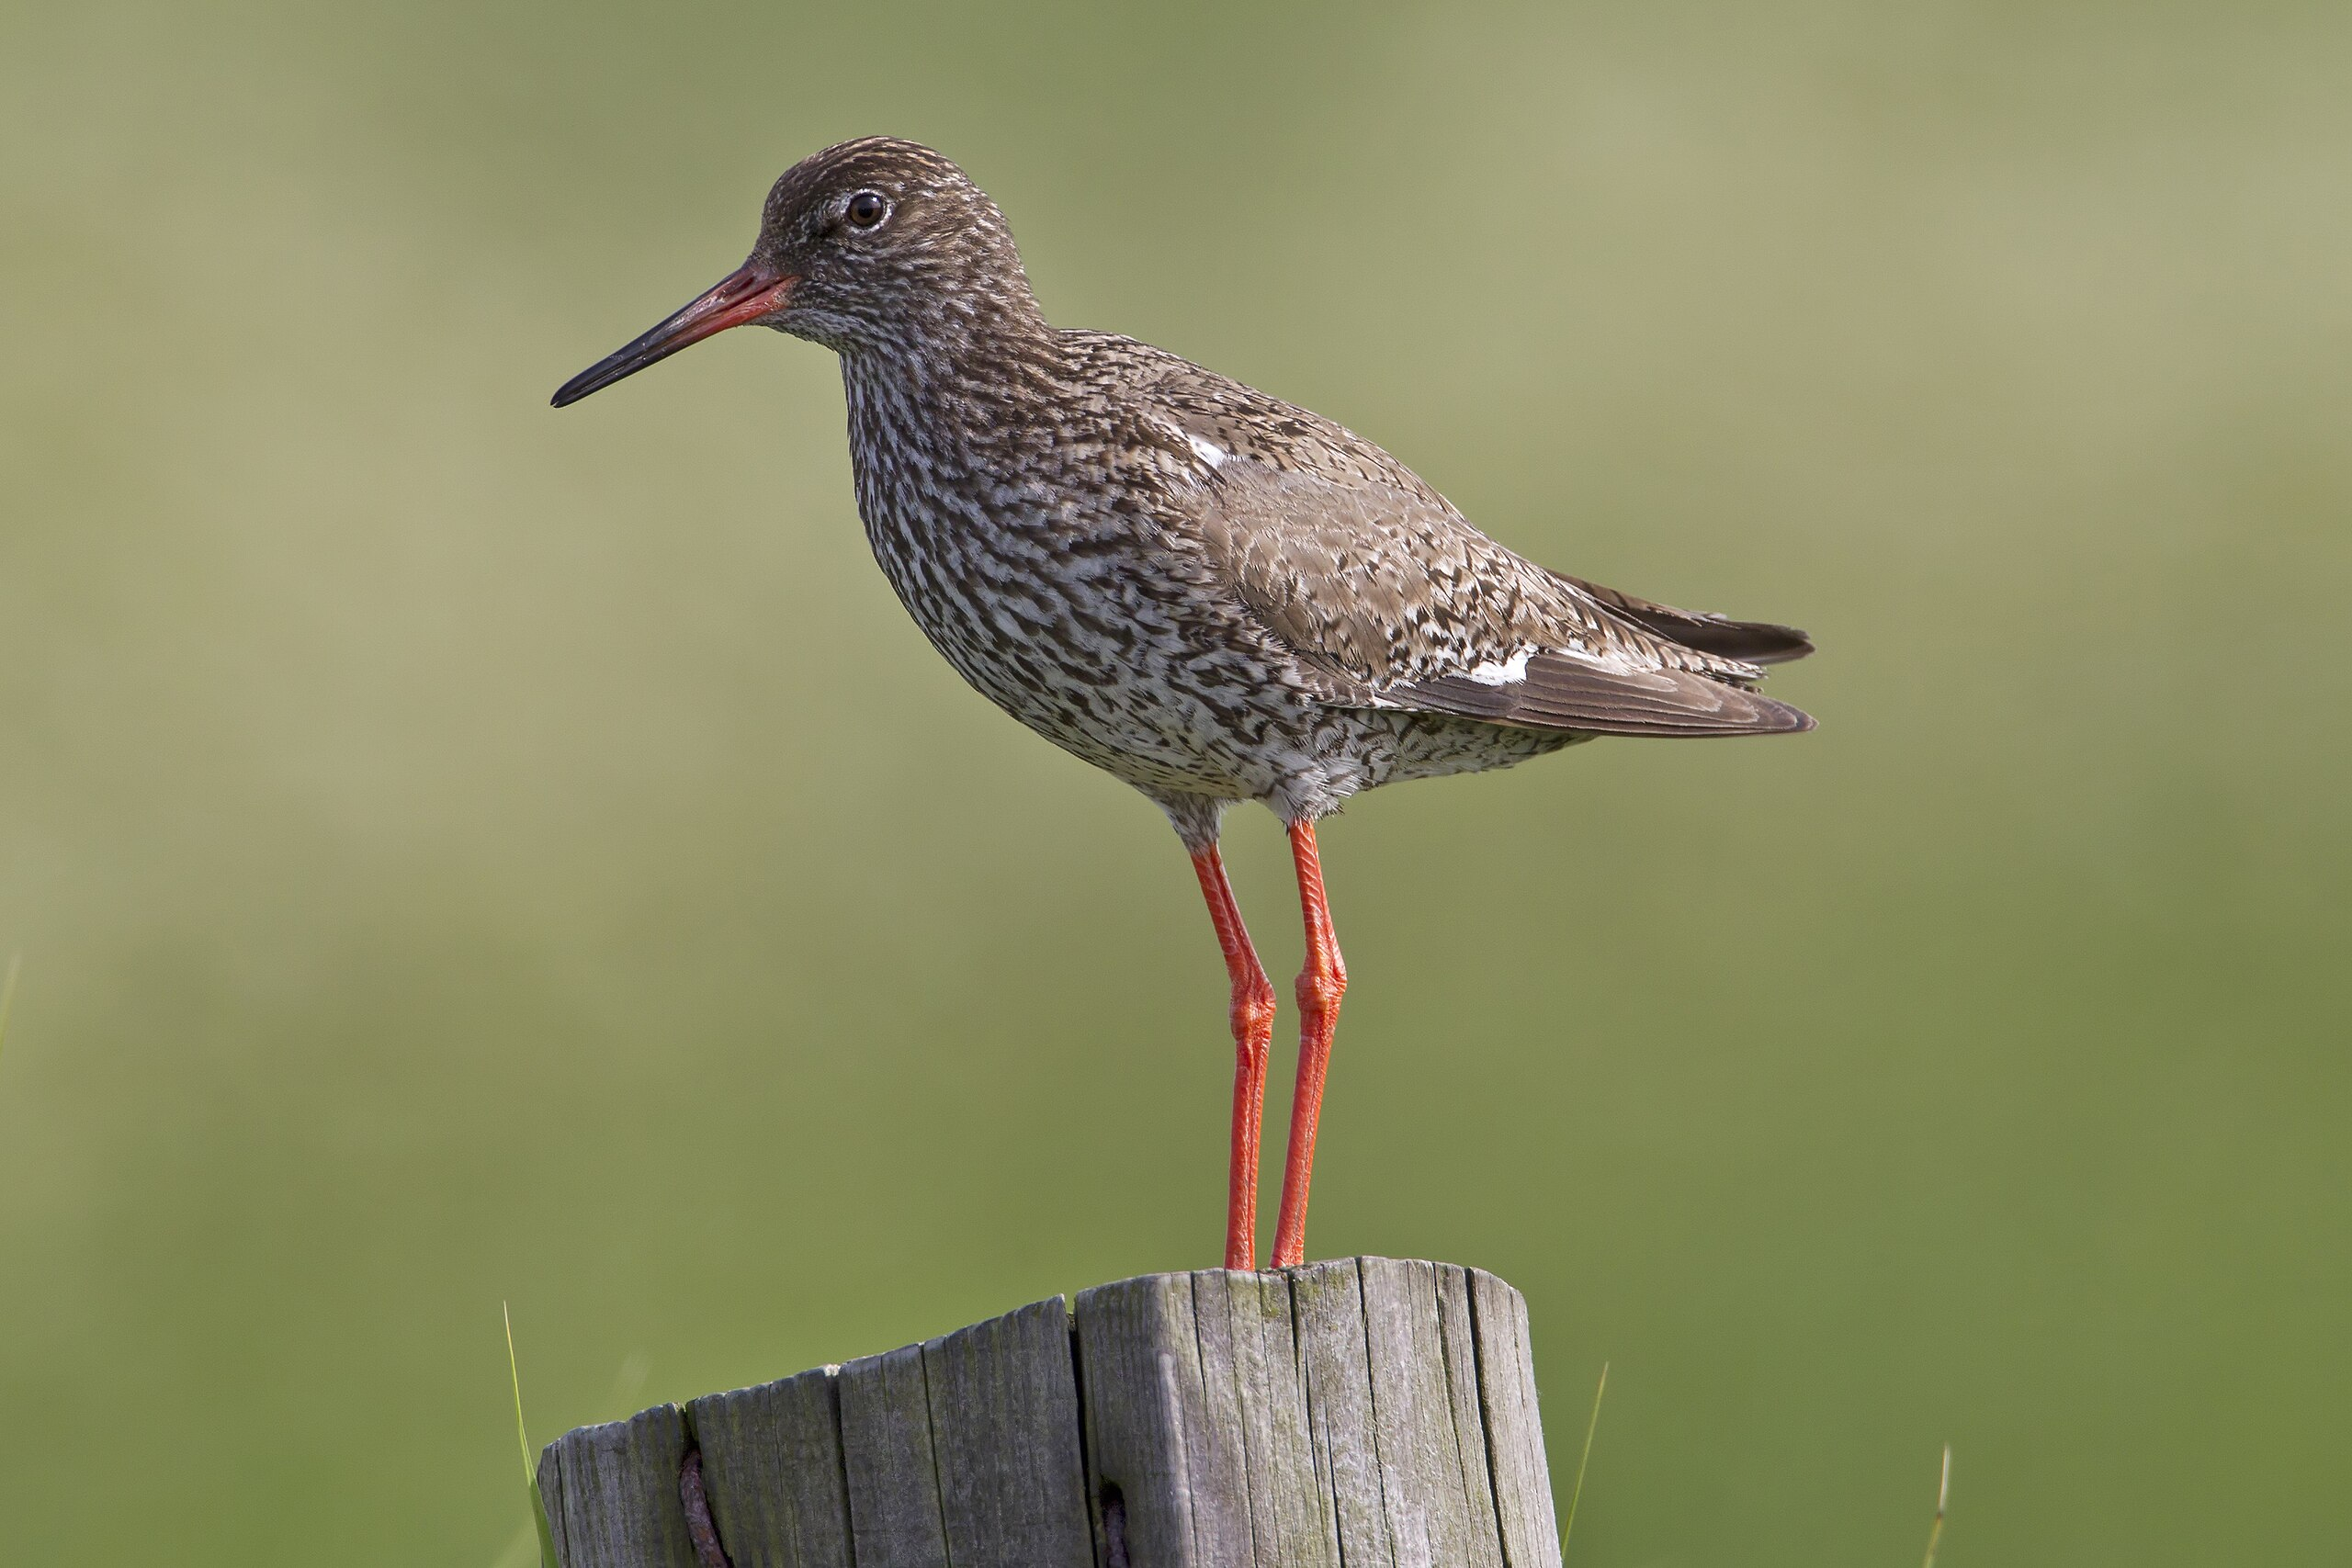
\includegraphics[width=0.8\linewidth, height=10cm, keepaspectratio]{Billeder/Dyr/Fugle/Vadefugle/rødben.jpg}
\end{minipage}
}%
\end{columns}
\end{frame}



\begin{frame}{%
  \begin{minipage}[t]{0.85\textwidth}
    Sortklire
  \end{minipage}%
  \hfill
  \begin{minipage}[t]{0.1\textwidth}
    \raggedleft
    
\includegraphics[width=0.55cm, height=0.55cm, keepaspectratio]{Billeder/Ikoner/star.png}%
  \end{minipage}%
} 
  \vspace{0.25em}
  \begin{columns}[T]
    % --- Venstre kolonne: Tekst ---
    \column{0.55\textwidth}
    \setlength{\parskip}{0.5em}
    \small
    \RaggedRight\textbf{\textit{Tringa erythropus}} – Ligner Rødben men har længere og tyndere næb \par

    \textbf{Udseende:} \\
    \quad – Sort fjerdragt med sorte/mørkerøde ben. Næbbet er lige med svagt dryppende spids. Prikker på oversiden af fjerdragten \par

    

    % --- Højre kolonne: To billeder stablet over hinanden ---
    \column{0.40\textwidth}
    \centering
    \fbox{%
      \begin{minipage}{\linewidth}
        \centering
        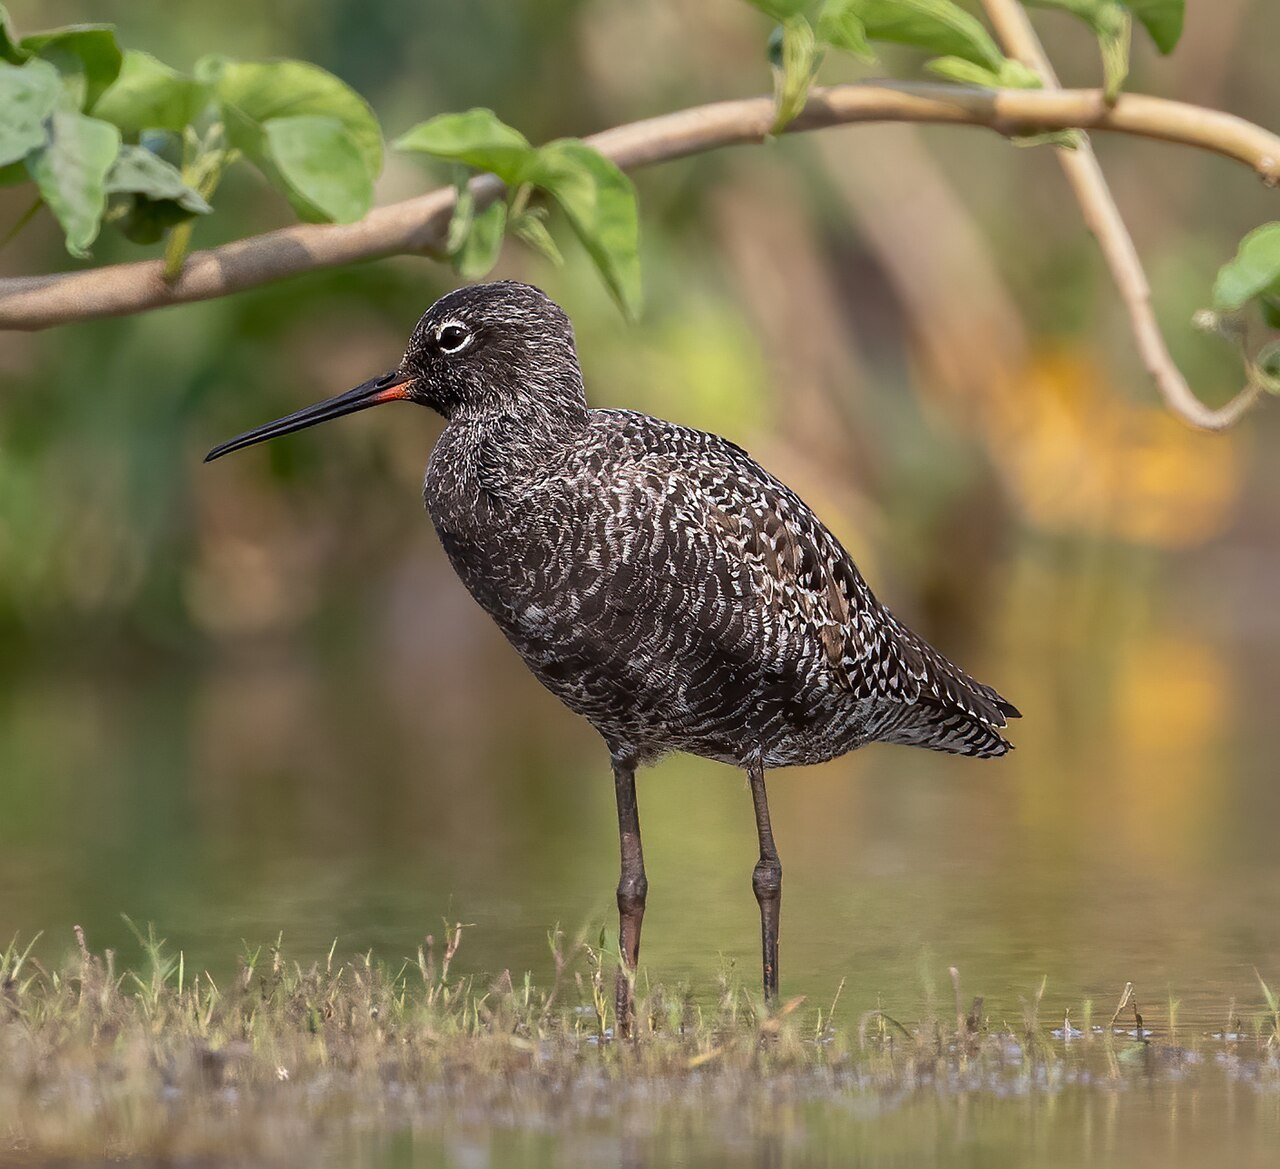
\includegraphics[width=0.8\linewidth, height=3cm, keepaspectratio]{Billeder/Dyr/Fugle/Vadefugle/sortklire_yngledragt.jpg}\\[0.5em]
        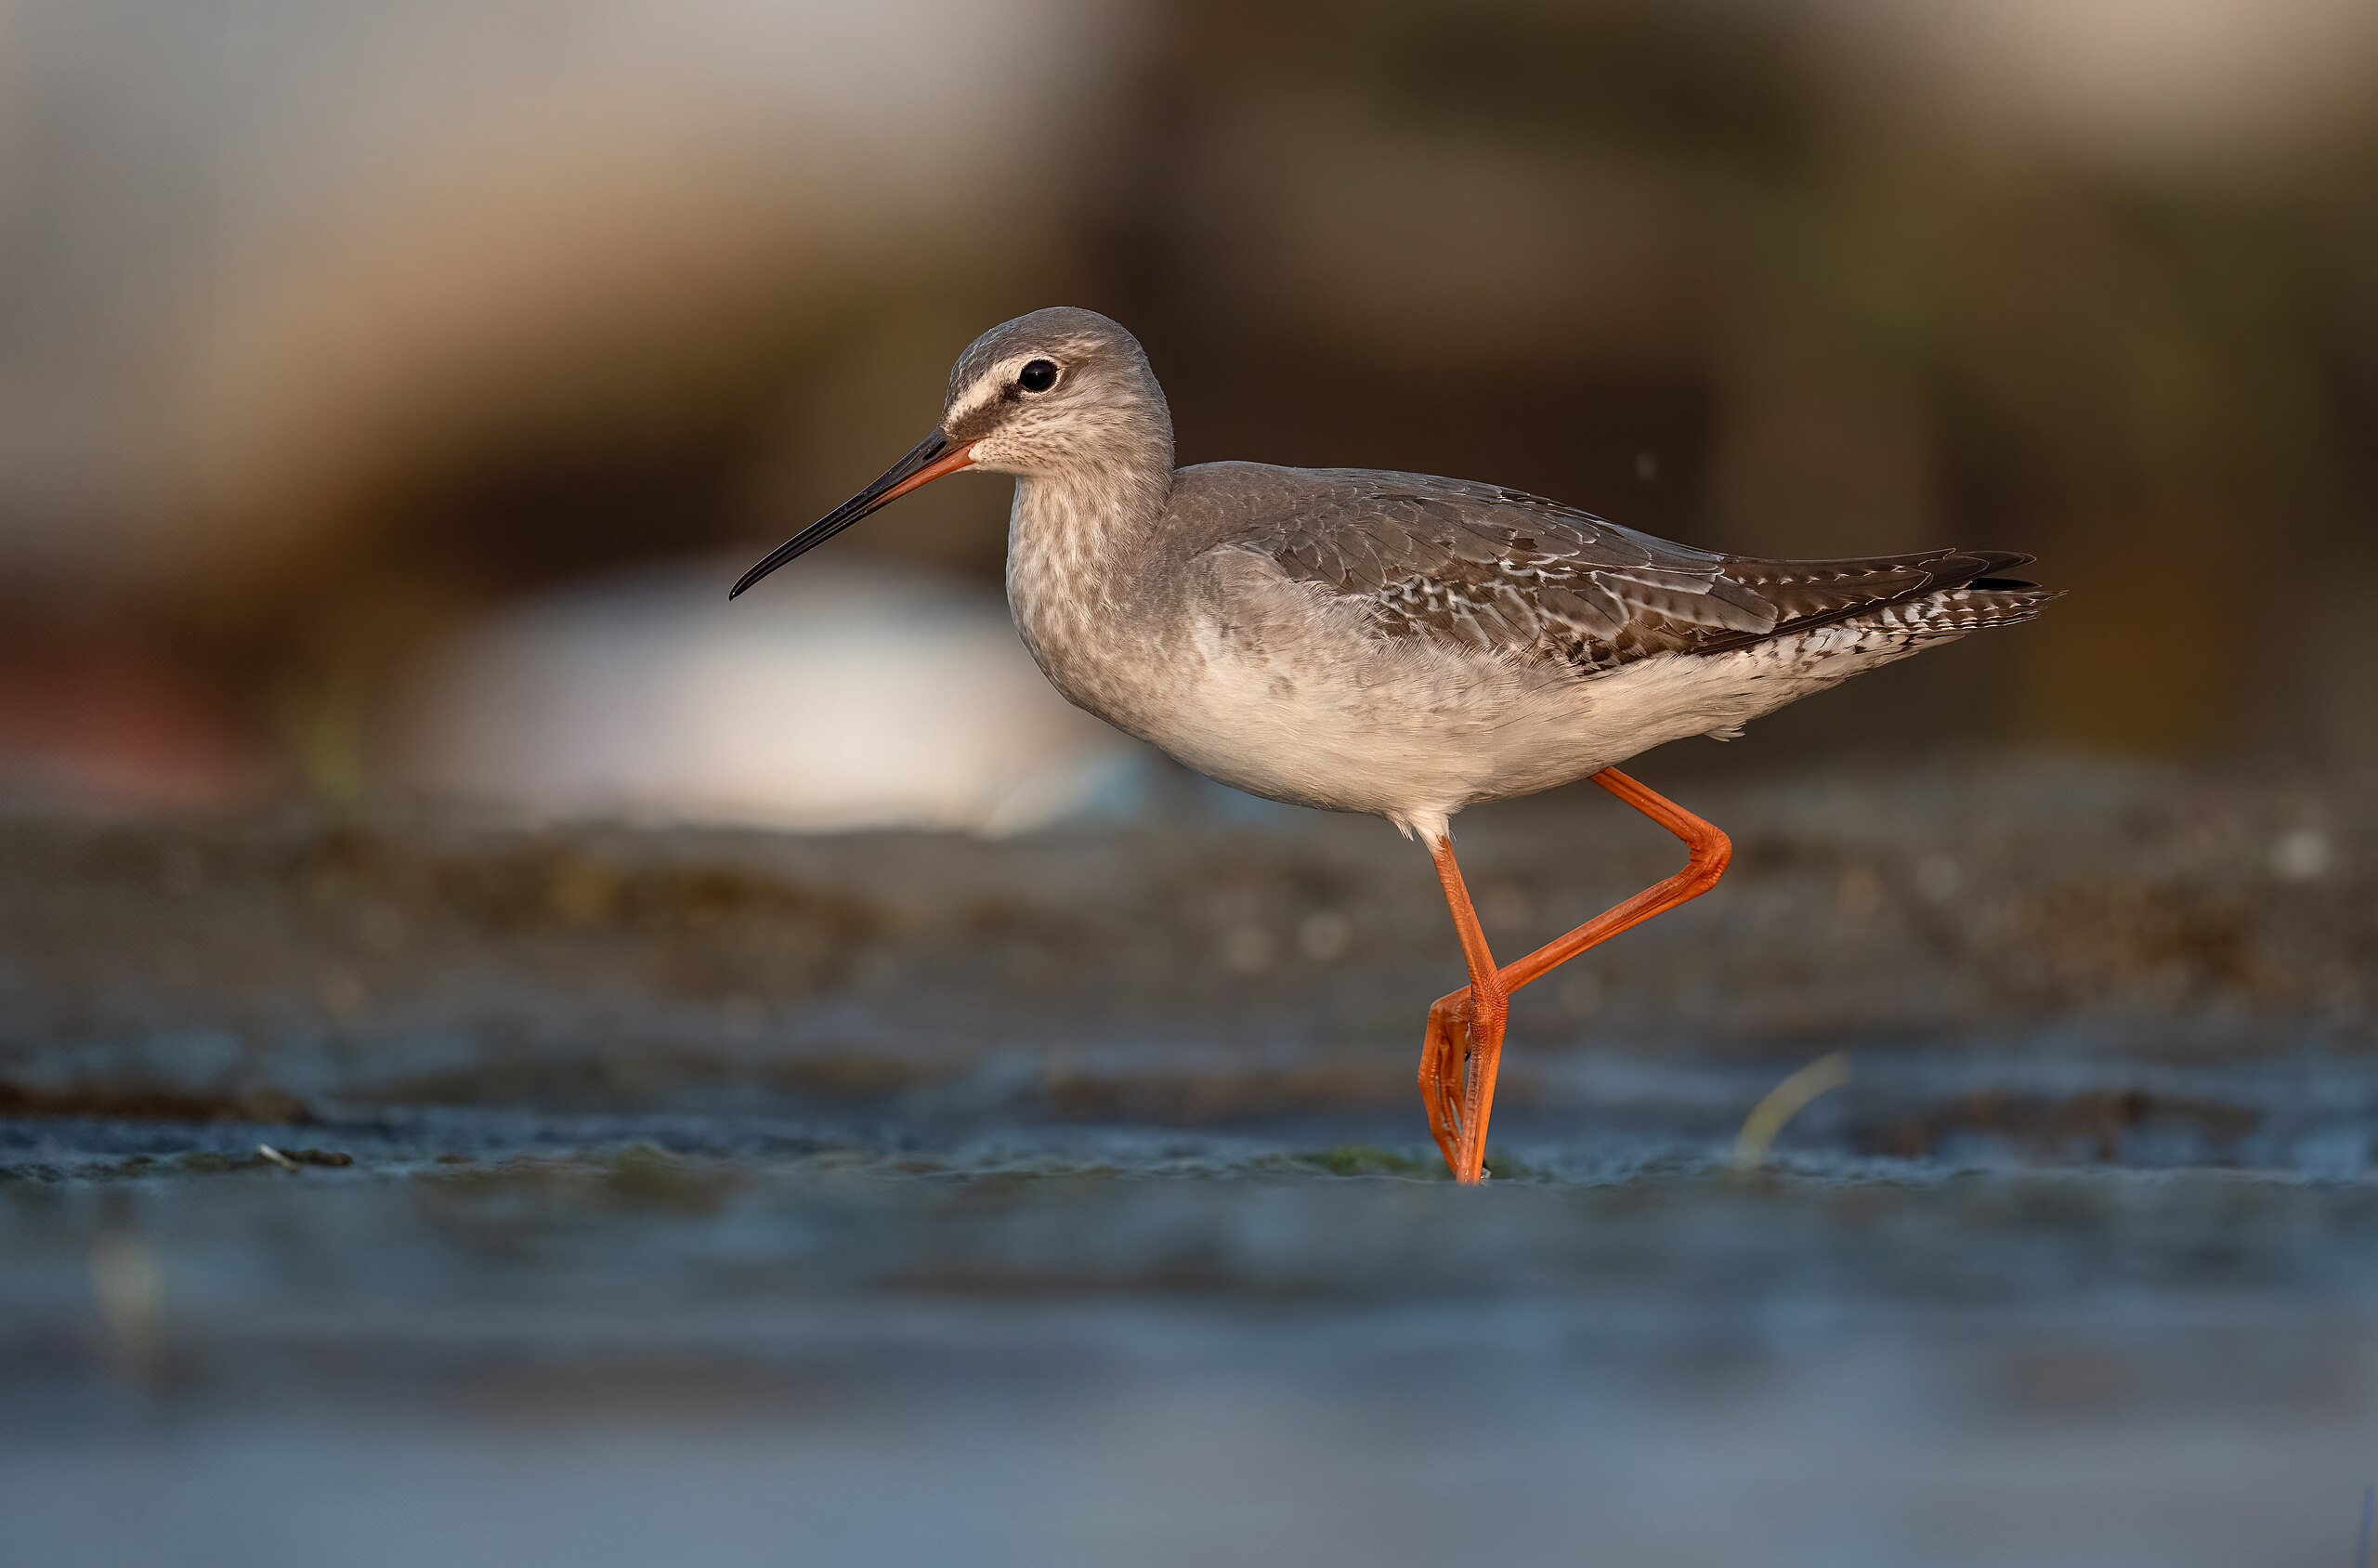
\includegraphics[width=0.8\linewidth, height=3cm, keepaspectratio]{Billeder/Dyr/Fugle/Vadefugle/sortklire_ungfugl.jpg}%
      \end{minipage}
    }%
    \vspace{0.05em}
    \footnotesize Sommer øverst, vinter nederst
  \end{columns}
\end{frame}



\begin{frame}{%
  \begin{minipage}[t]{0.85\textwidth}
    Hvidklire
  \end{minipage}%
  \hfill
  \begin{minipage}[t]{0.1\textwidth}
    \raggedleft
    
\includegraphics[width=0.55cm, height=0.55cm, keepaspectratio]{Billeder/Ikoner/star.png}%
  \end{minipage}%
} 
  \vspace{0.25em}
  \begin{columns}[T]
    % --- Venstre kolonne: Tekst ---
    \column{0.55\textwidth}
    \setlength{\parskip}{0.5em}
    \small
    \RaggedRight\textbf{\textit{Tringa nebularia}} – Trækfugl i Danmark som før hed grønben \par

    \textbf{Udseende:} \\
    \quad – Grønne ben og langt grågrønt let opadbuet næb

    

    % --- Højre kolonne: To billeder stablet over hinanden ---
    \column{0.40\textwidth}
    \centering
    \fbox{%
      \begin{minipage}{\linewidth}
        \centering
        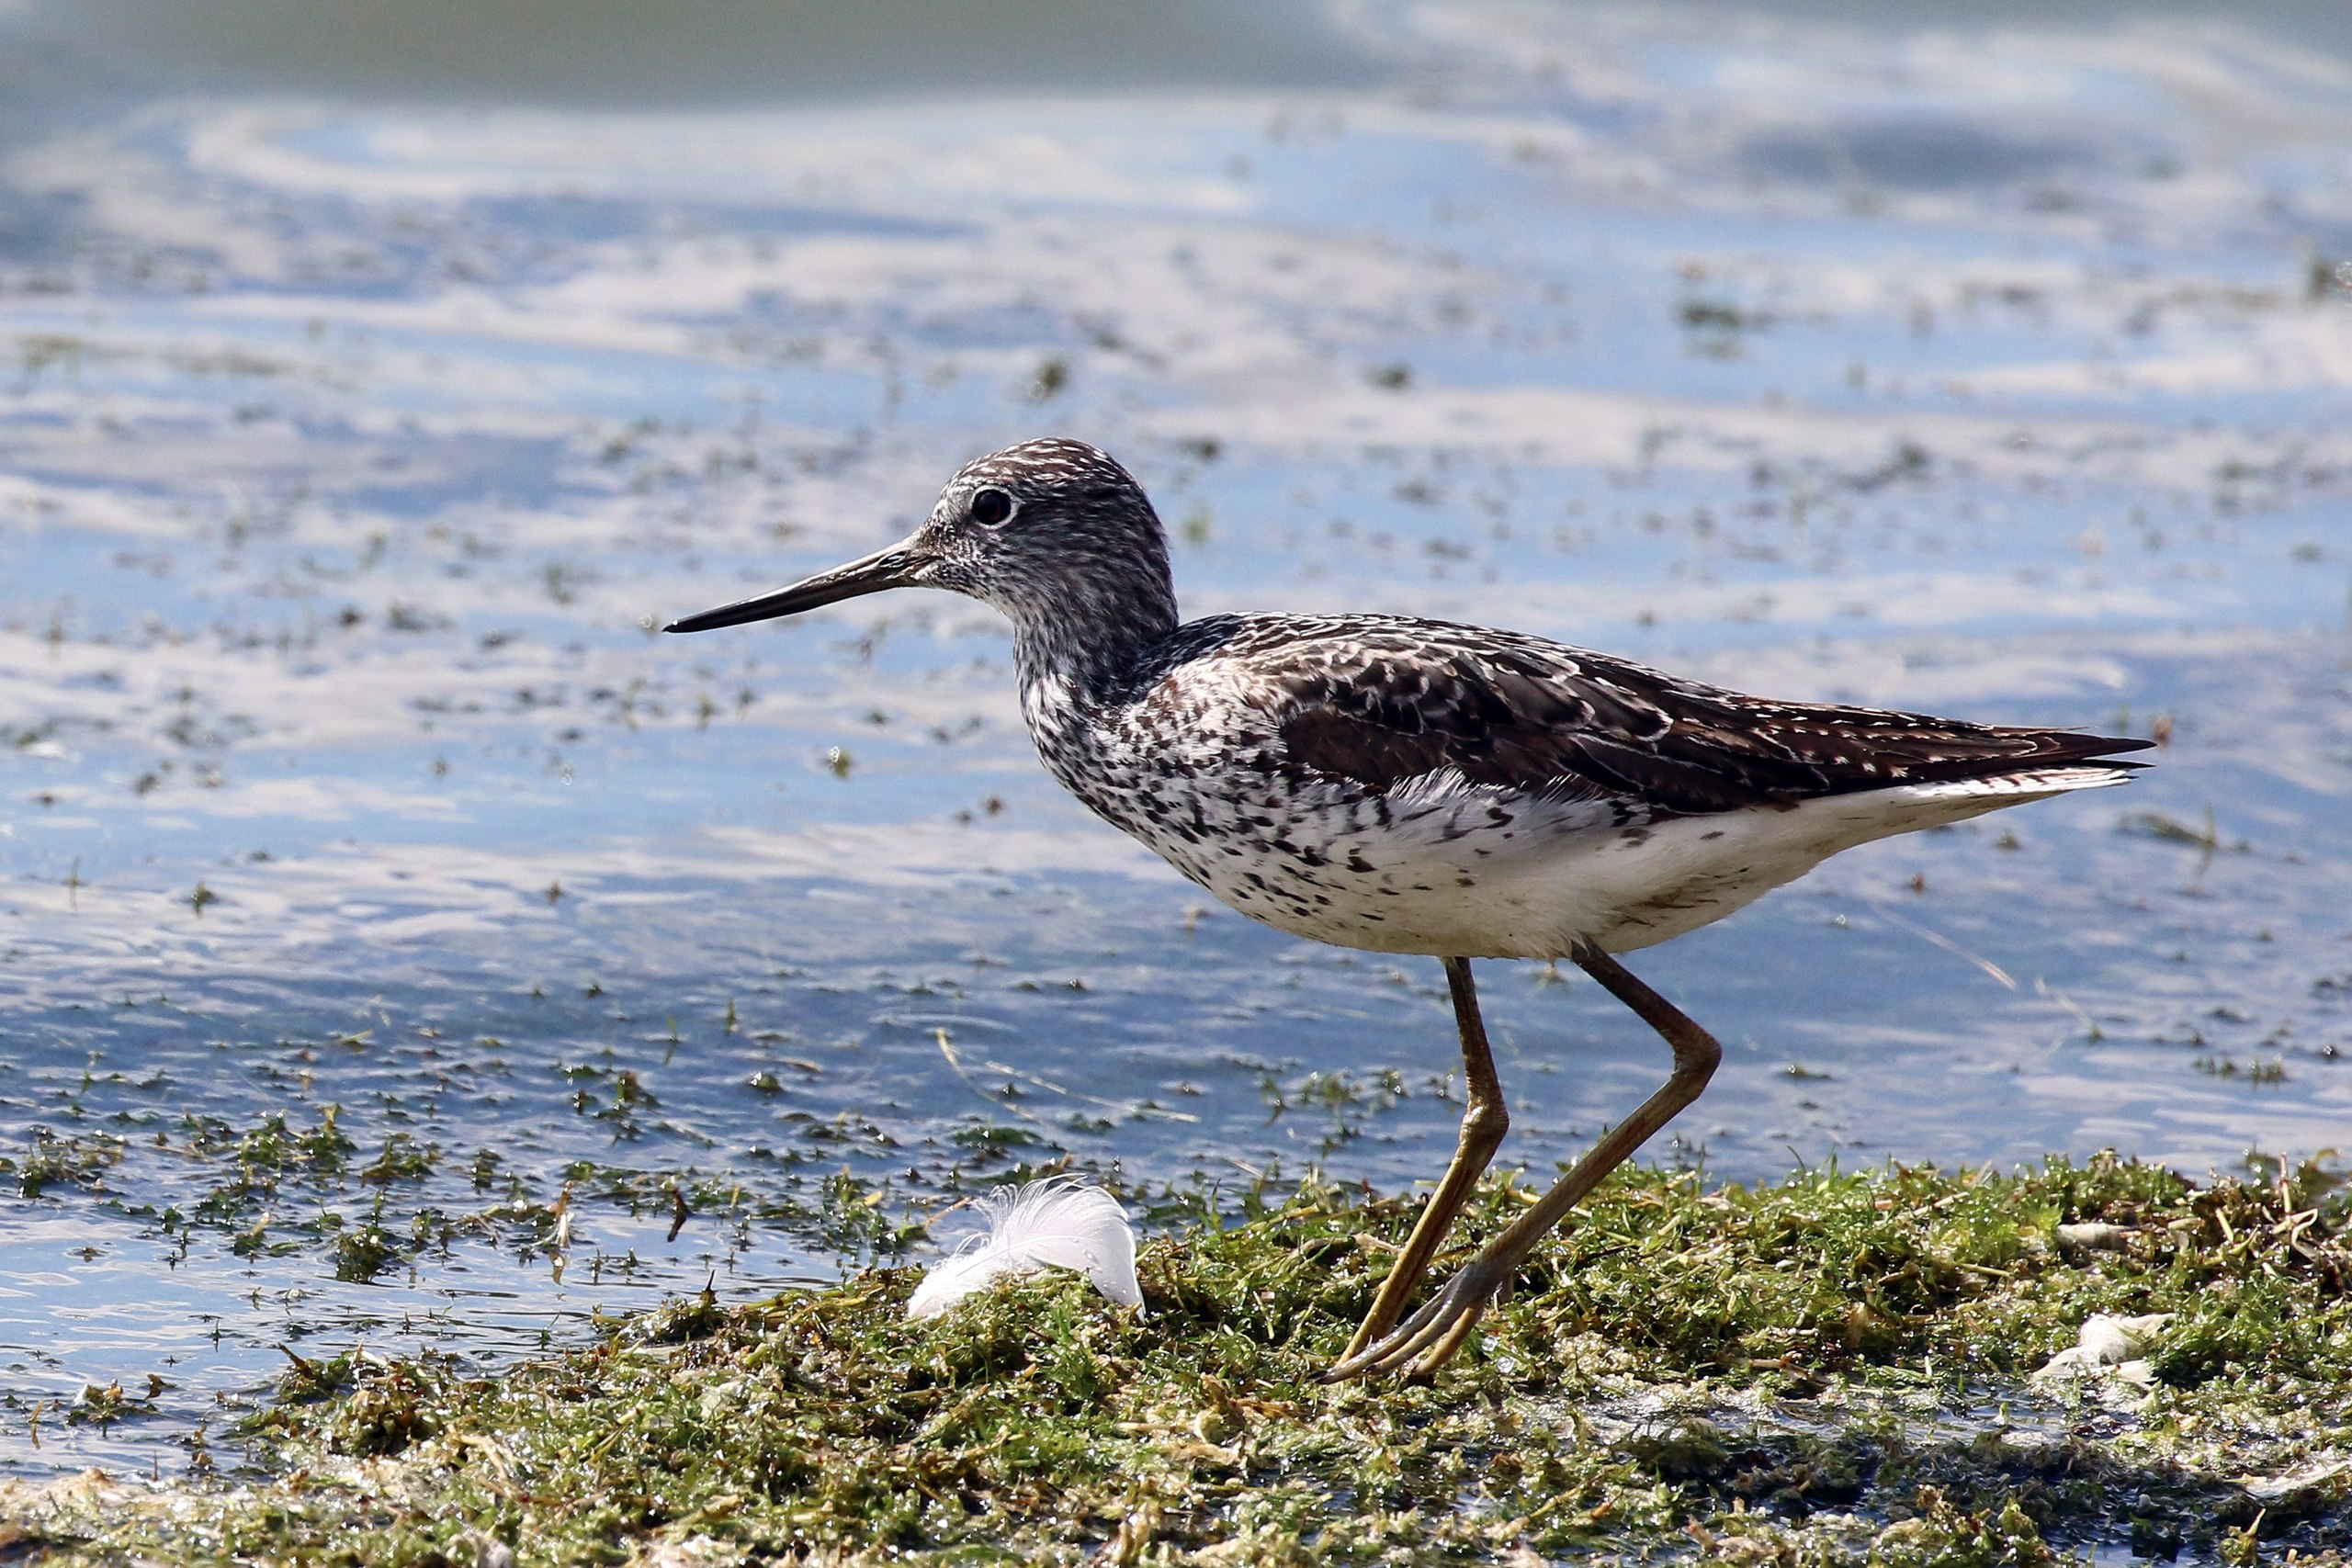
\includegraphics[width=0.8\linewidth, height=3cm, keepaspectratio]{Billeder/Dyr/Fugle/Vadefugle/hvidklire_sommer.jpg}\\[0.5em]
        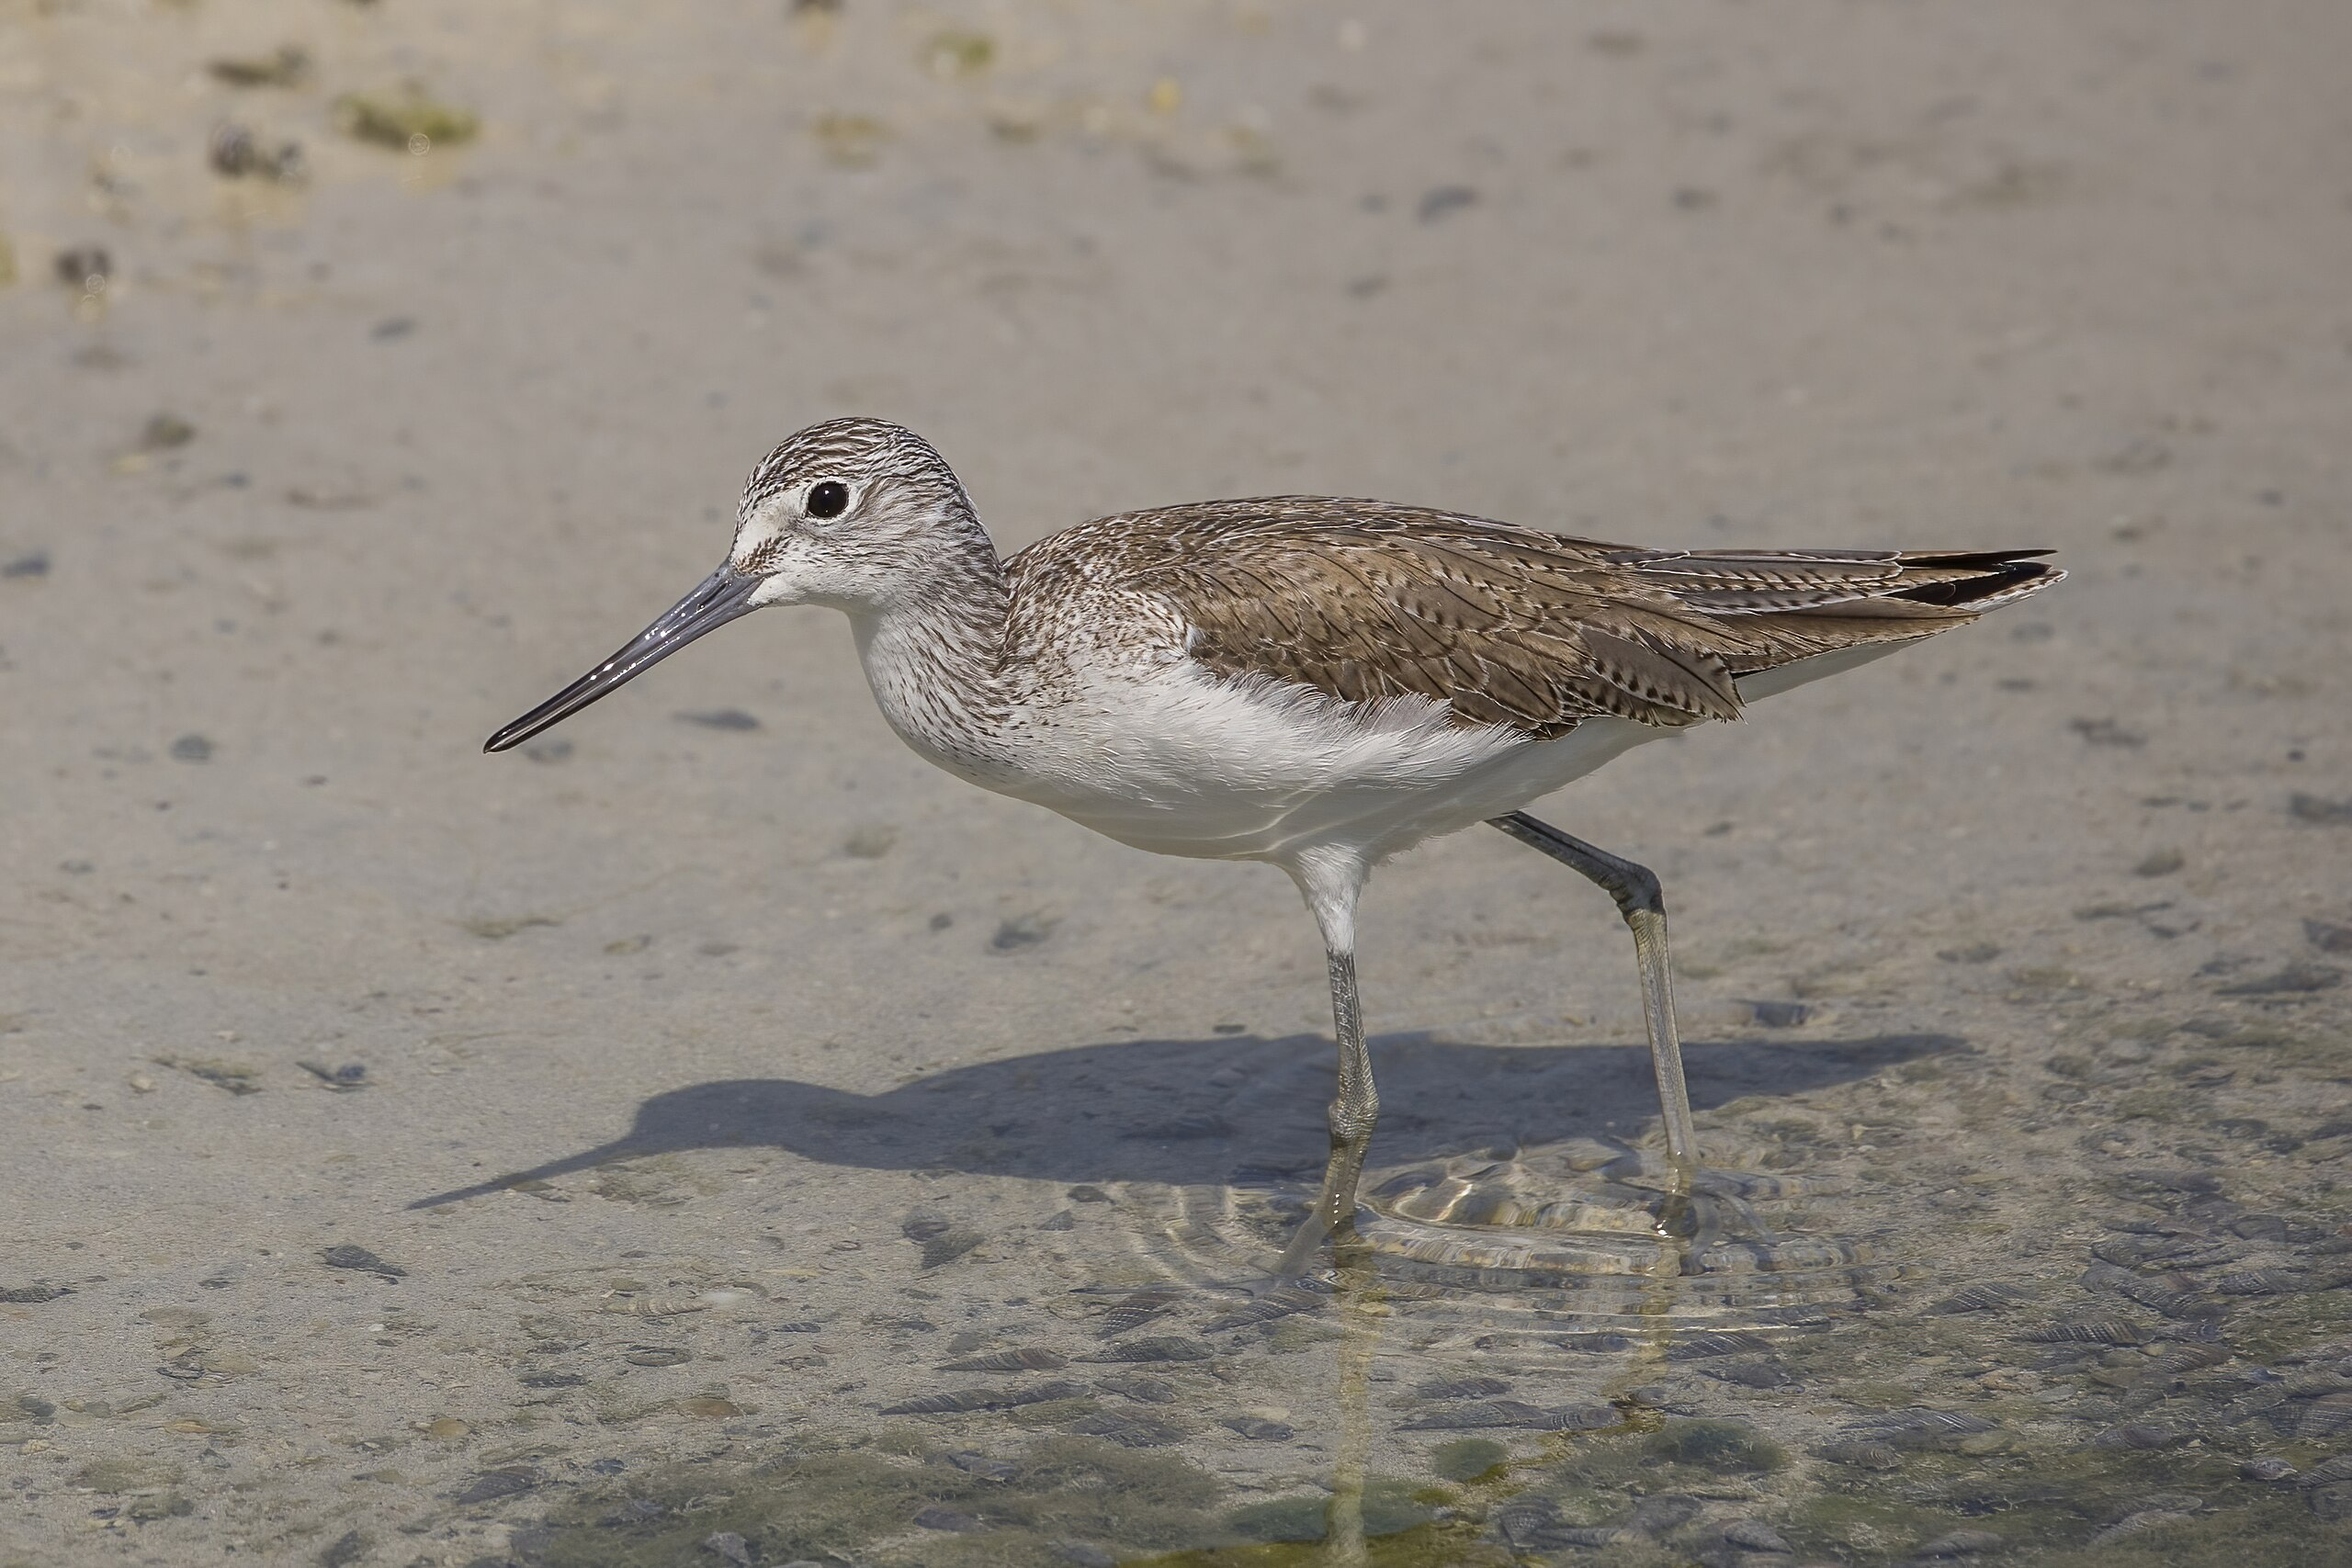
\includegraphics[width=0.8\linewidth, height=3cm, keepaspectratio]{Billeder/Dyr/Fugle/Vadefugle/hvidklire_vinter.jpg}%
      \end{minipage}
    }%
    \vspace{0.05em}
    \footnotesize Sommer fjerdragt øverst, vinter nederst
  \end{columns}
\end{frame}
\begin{frame}{%
\begin{minipage}[t]{0.85\textwidth}
Islandsk ryle
\end{minipage}%
\hfill
\begin{minipage}[t]{0.1\textwidth}
\raggedleft

\includegraphics[width=0.55cm, height=0.55cm, keepaspectratio]{Billeder/Ikoner/star.png}%
\end{minipage}%
}
\vspace{0.25em}
\begin{columns}[T]
% --- Venstre kolonne: Tekst ---
\column{0.55\textwidth}
\setlength{\parskip}{0.5em}
\small
\RaggedRight\textbf{\textit{Calidris canutus}} – Kortbenet kraftig vadefugl med kort næb\par

\textbf{Udseende:} \\
\quad –  Kort, mørkt næb og grågrønne ben  

% --- Højre kolonne: Et billede ---
\column{0.40\textwidth}
\centering
\fbox{%
\begin{minipage}{\linewidth}
\centering
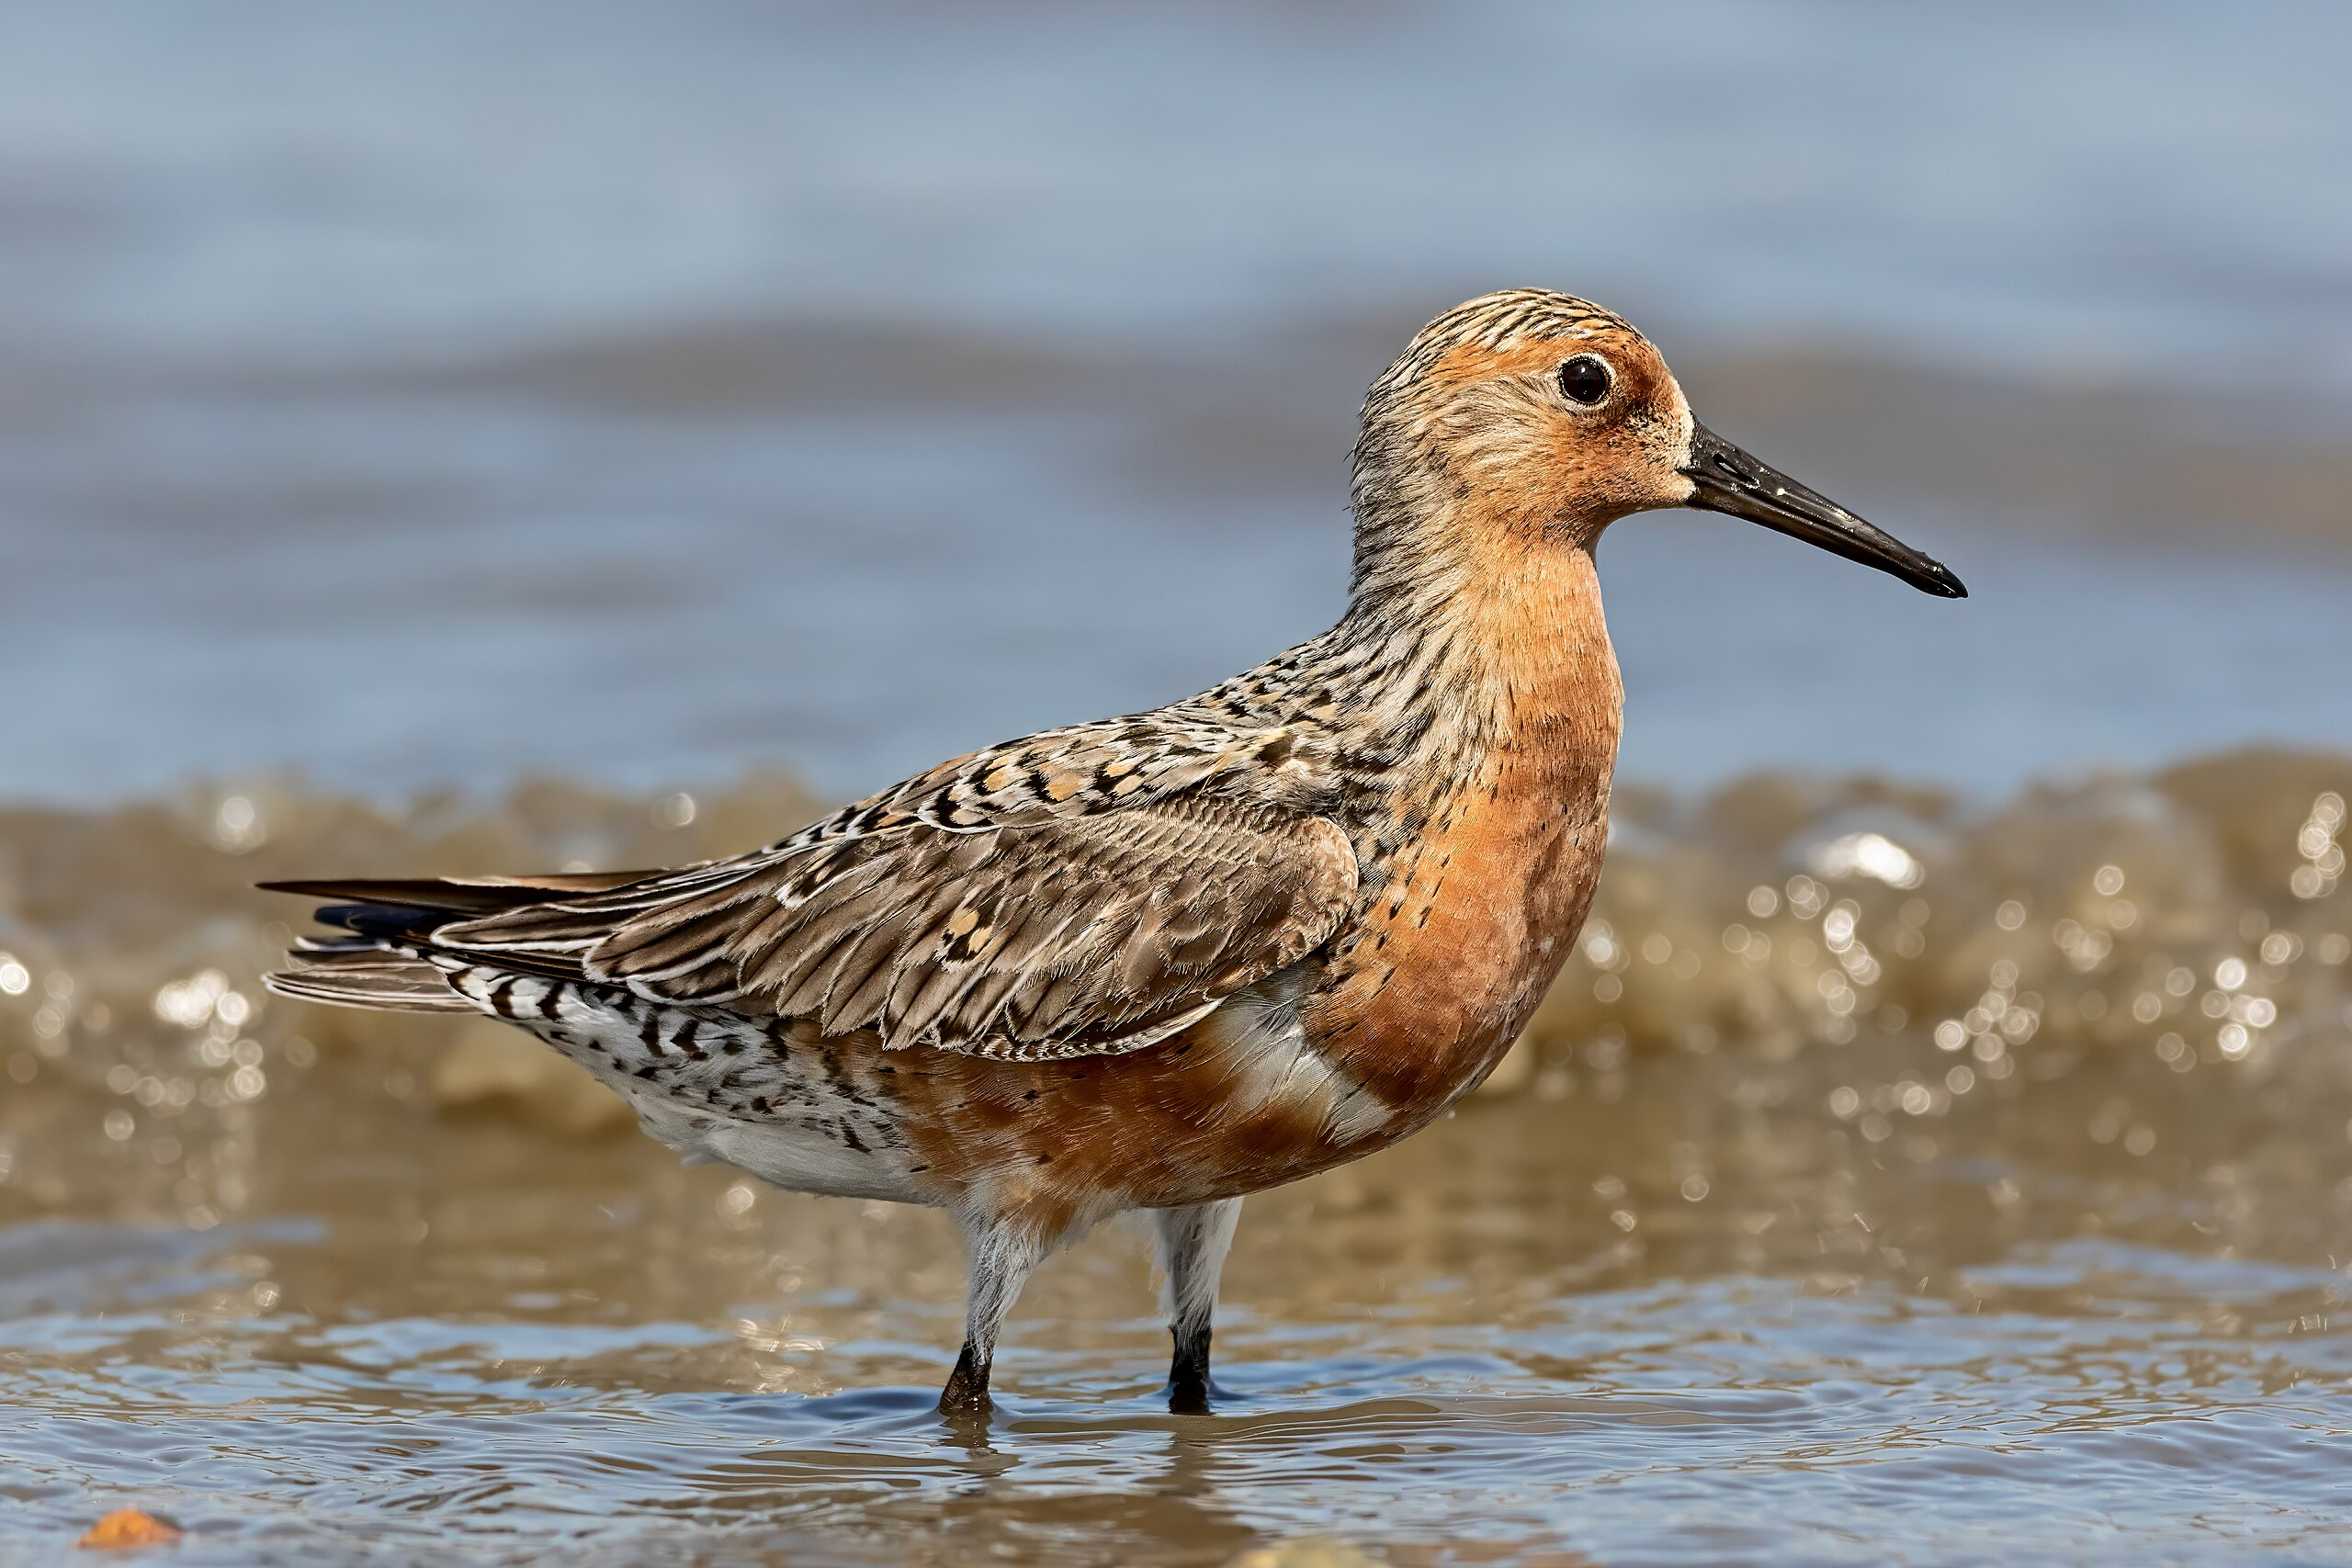
\includegraphics[width=0.8\linewidth, height=10cm, keepaspectratio]{Billeder/Dyr/Fugle/Vadefugle/islandsk_ryle.jpg}
\end{minipage}
}%
\end{columns}
\end{frame}



\begin{frame}{%
  \begin{minipage}[t]{0.85\textwidth}
    Brushane
  \end{minipage}%
  \hfill
  \begin{minipage}[t]{0.1\textwidth}
    \raggedleft
    
\includegraphics[width=0.55cm, height=0.55cm, keepaspectratio]{Billeder/Ikoner/star.png}%
  \end{minipage}%
} 
  \vspace{0.25em}
  \begin{columns}[T]
    % --- Venstre kolonne: Tekst ---
    \column{0.55\textwidth}
    \setlength{\parskip}{0.5em}
    \small
    \RaggedRight\textbf{\textit{Calidris pugnax}} – stor vadefugl som tilhører sneppefuglene \par

    \textbf{Udseende:} \\
    \quad – Kort svagt nedadbøjet næb. Giraf-hals. Uproportionelt lille hoved ift. krop. 

    

    % --- Højre kolonne: To billeder stablet over hinanden ---
    \column{0.40\textwidth}
    \centering
    \fbox{%
      \begin{minipage}{\linewidth}
        \centering
        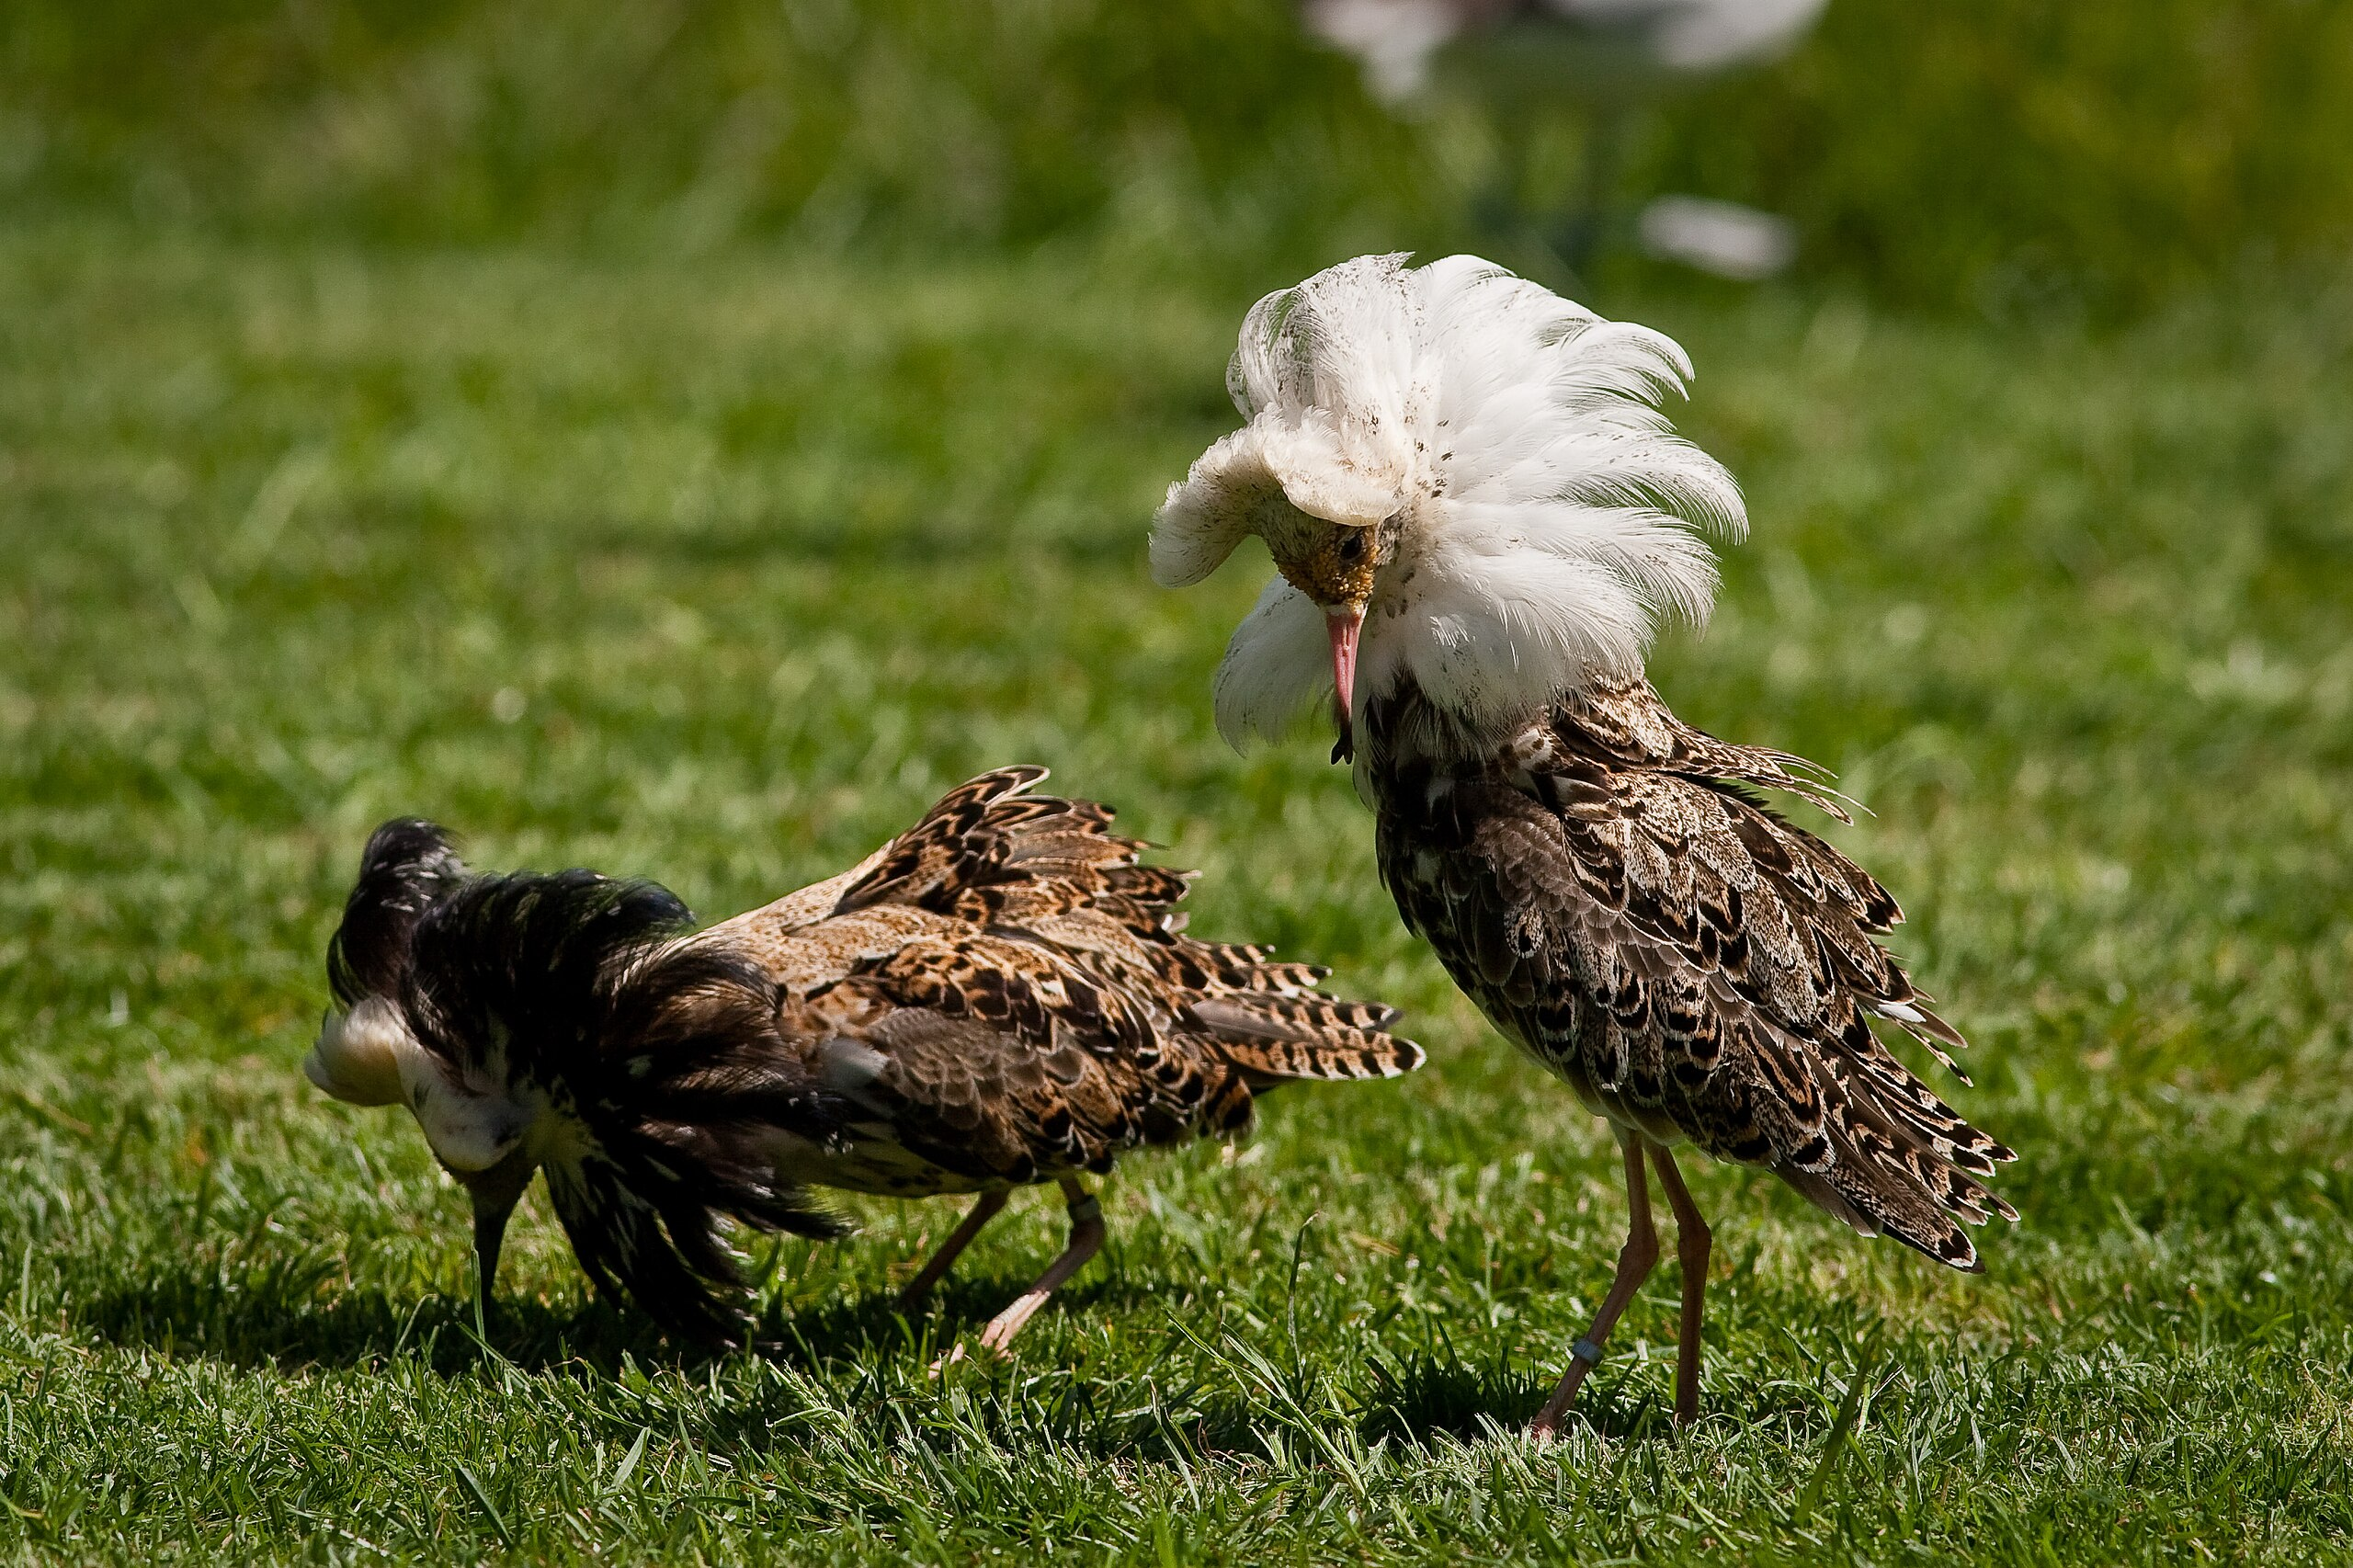
\includegraphics[width=0.8\linewidth, height=3cm, keepaspectratio]{Billeder/Dyr/Fugle/Vadefugle/brushane_han.jpg}\\[0.5em]
        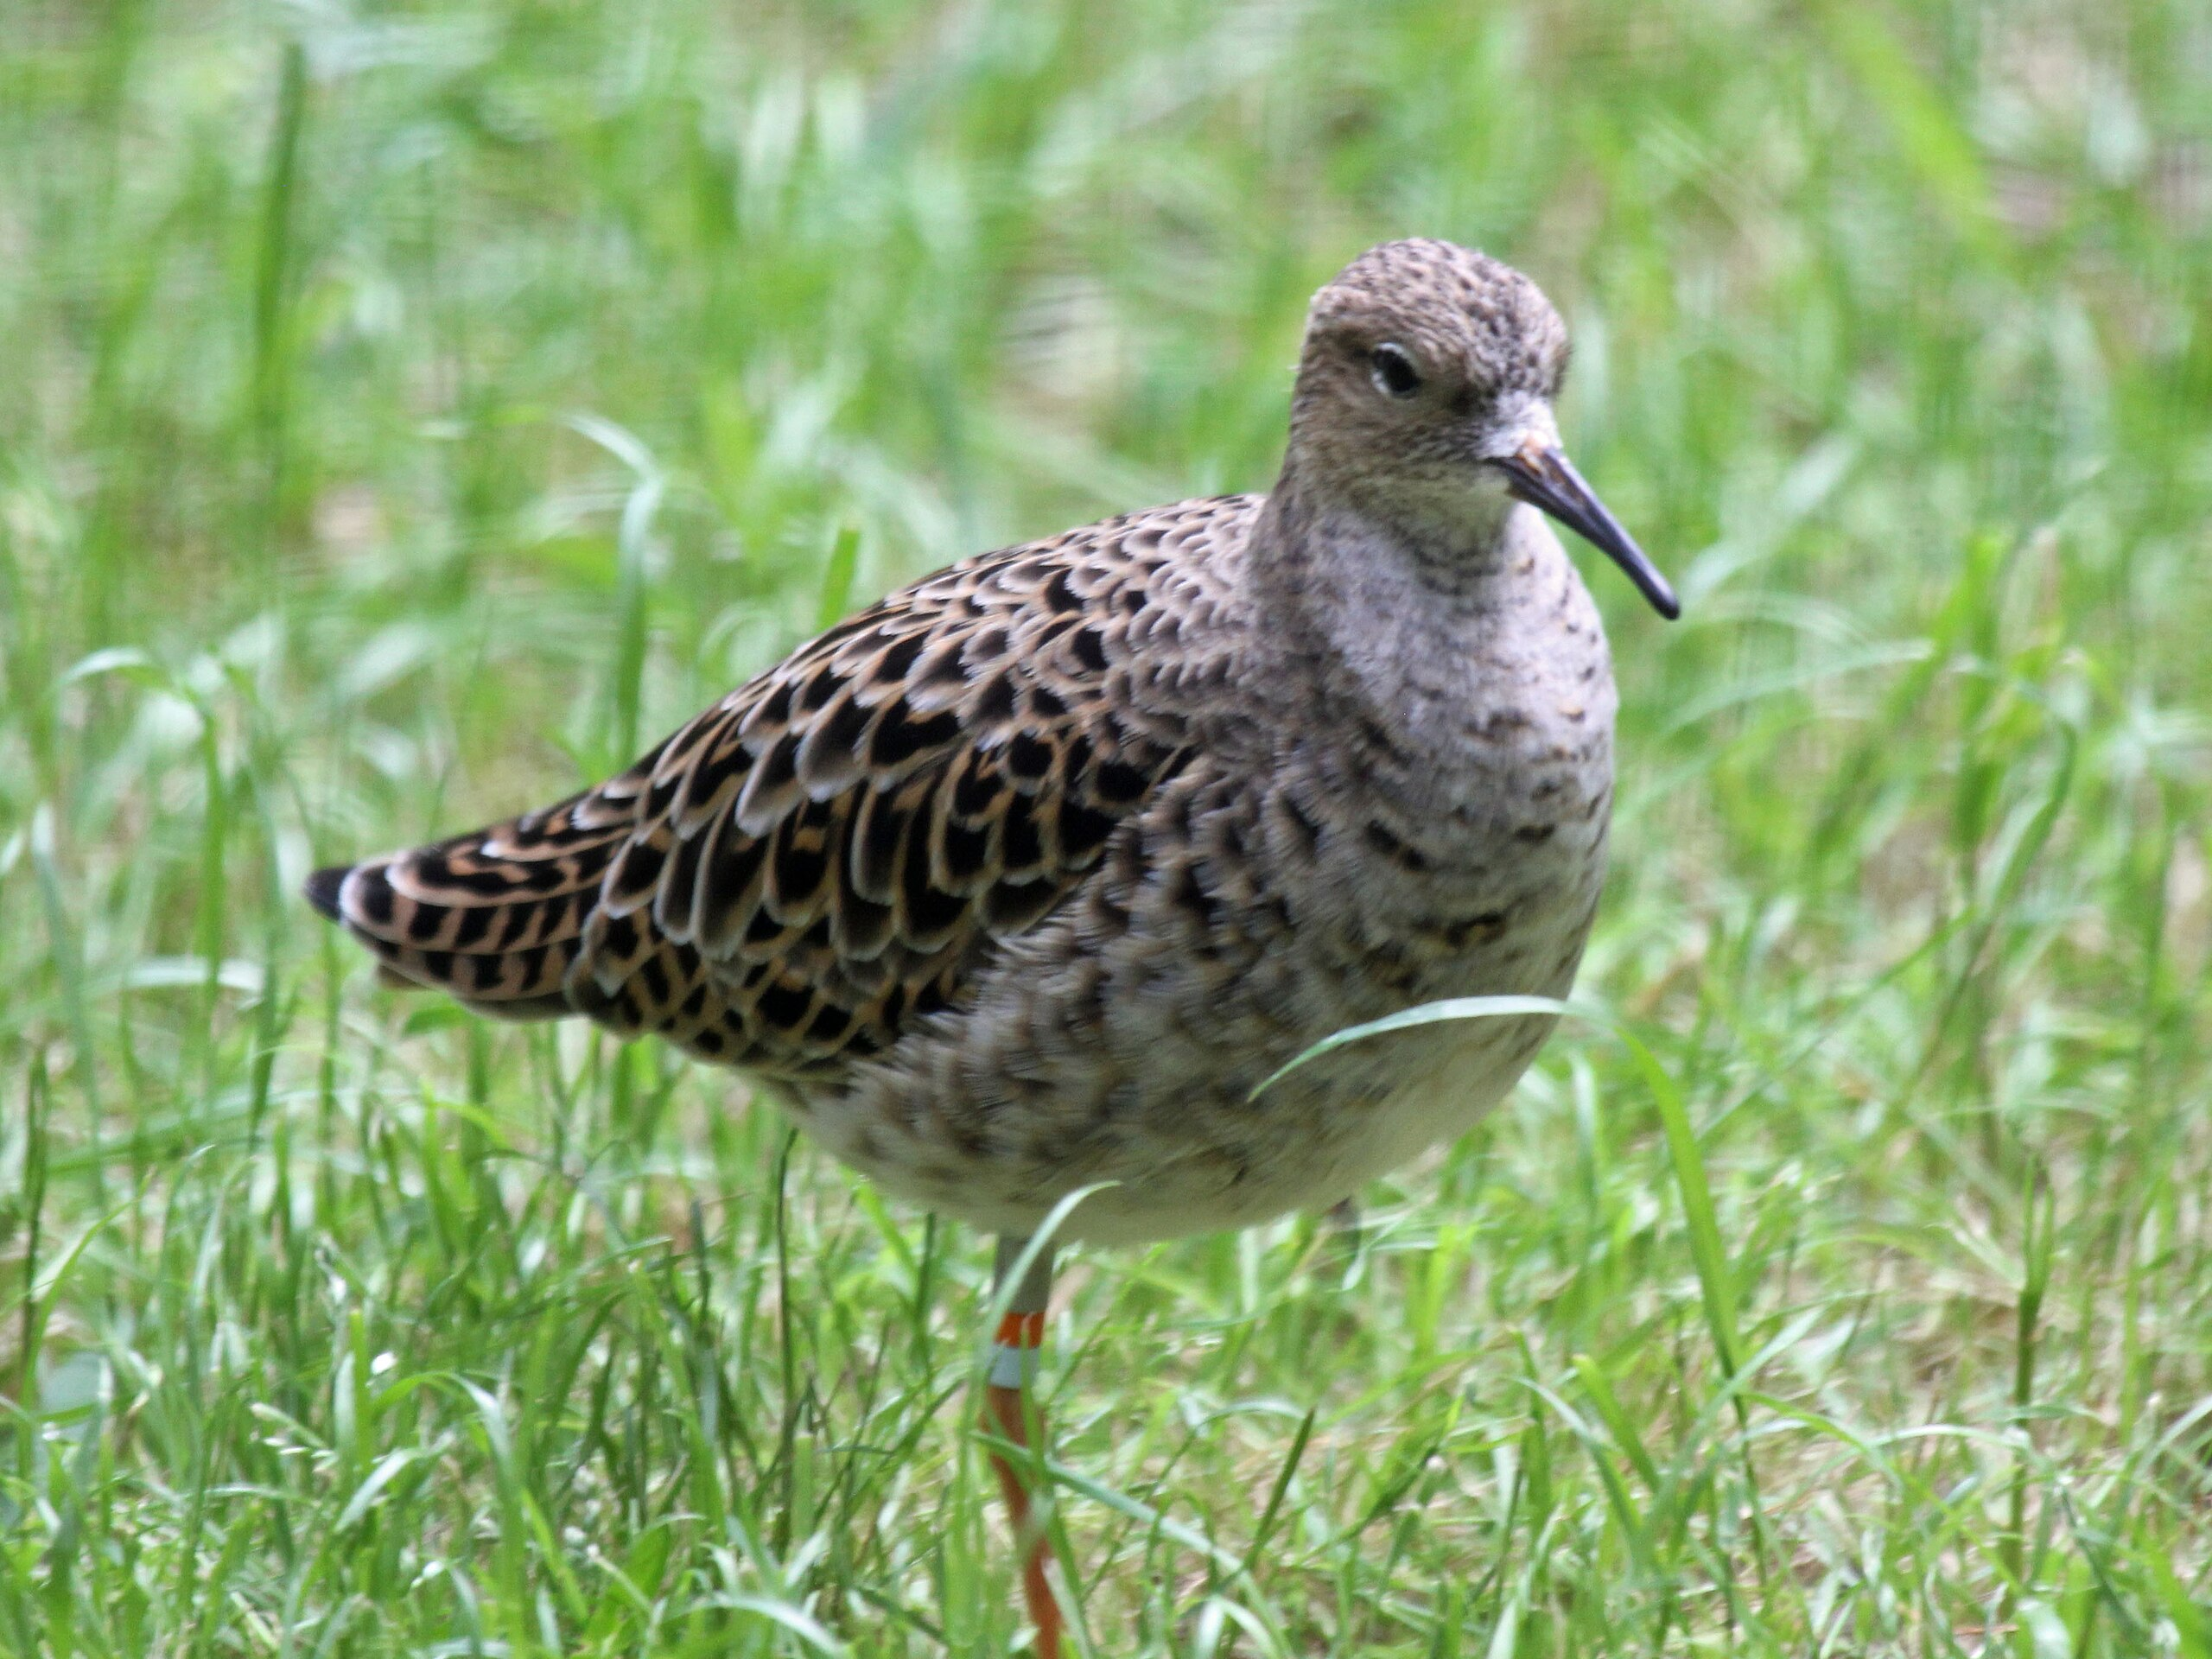
\includegraphics[width=0.8\linewidth, height=3cm, keepaspectratio]{Billeder/Dyr/Fugle/Vadefugle/brushane_hun.jpg}%
      \end{minipage}
    }%
    \vspace{0.05em}
    \footnotesize Han øverst, hun nederst
  \end{columns}
\end{frame}
\begin{frame}{%
\begin{minipage}[t]{0.85\textwidth}
Dobbeltbekkasin
\end{minipage}%
\hfill
\begin{minipage}[t]{0.1\textwidth}
\raggedleft

\includegraphics[width=0.5cm, height=0.5cm, keepaspectratio]{Billeder/Ikoner/star.png}%
\hspace{0.2em}%

\includegraphics[width=0.5cm, height=0.5cm, keepaspectratio]{Billeder/Ikoner/star.png}
\end{minipage}%
}
\vspace{0.25em}
\begin{columns}[T]
% --- Venstre kolonne: Tekst ---
\column{0.55\textwidth}
\setlength{\parskip}{0.5em}
\small
\RaggedRight\textbf{\textit{Gallinago gallinago}} – På størrelse med solsort med meget langt næb\par 

\textbf{Udseende:} \\
\quad –  Brun ryg med gule længdestriber. Mørkebrun isse med gule issestribe. Næb mere end dobbelt så langt som hoved \par

\textbf{Levesteder:} \\
\quad – Engarealer, marsk og moser \par

\textbf{Føde:} \\
\quad – Insekter, biller, larver, orme \par

\textbf{Udbredelse:} \\
\quad – I hele landet \par

\textbf{Træk/standfugl} \\
\quad – Begge \par

% --- Højre kolonne: Kun ét billede (Hannen) ---
\column{0.40\textwidth}
\centering
\fbox{%
\begin{minipage}{\linewidth}
\centering
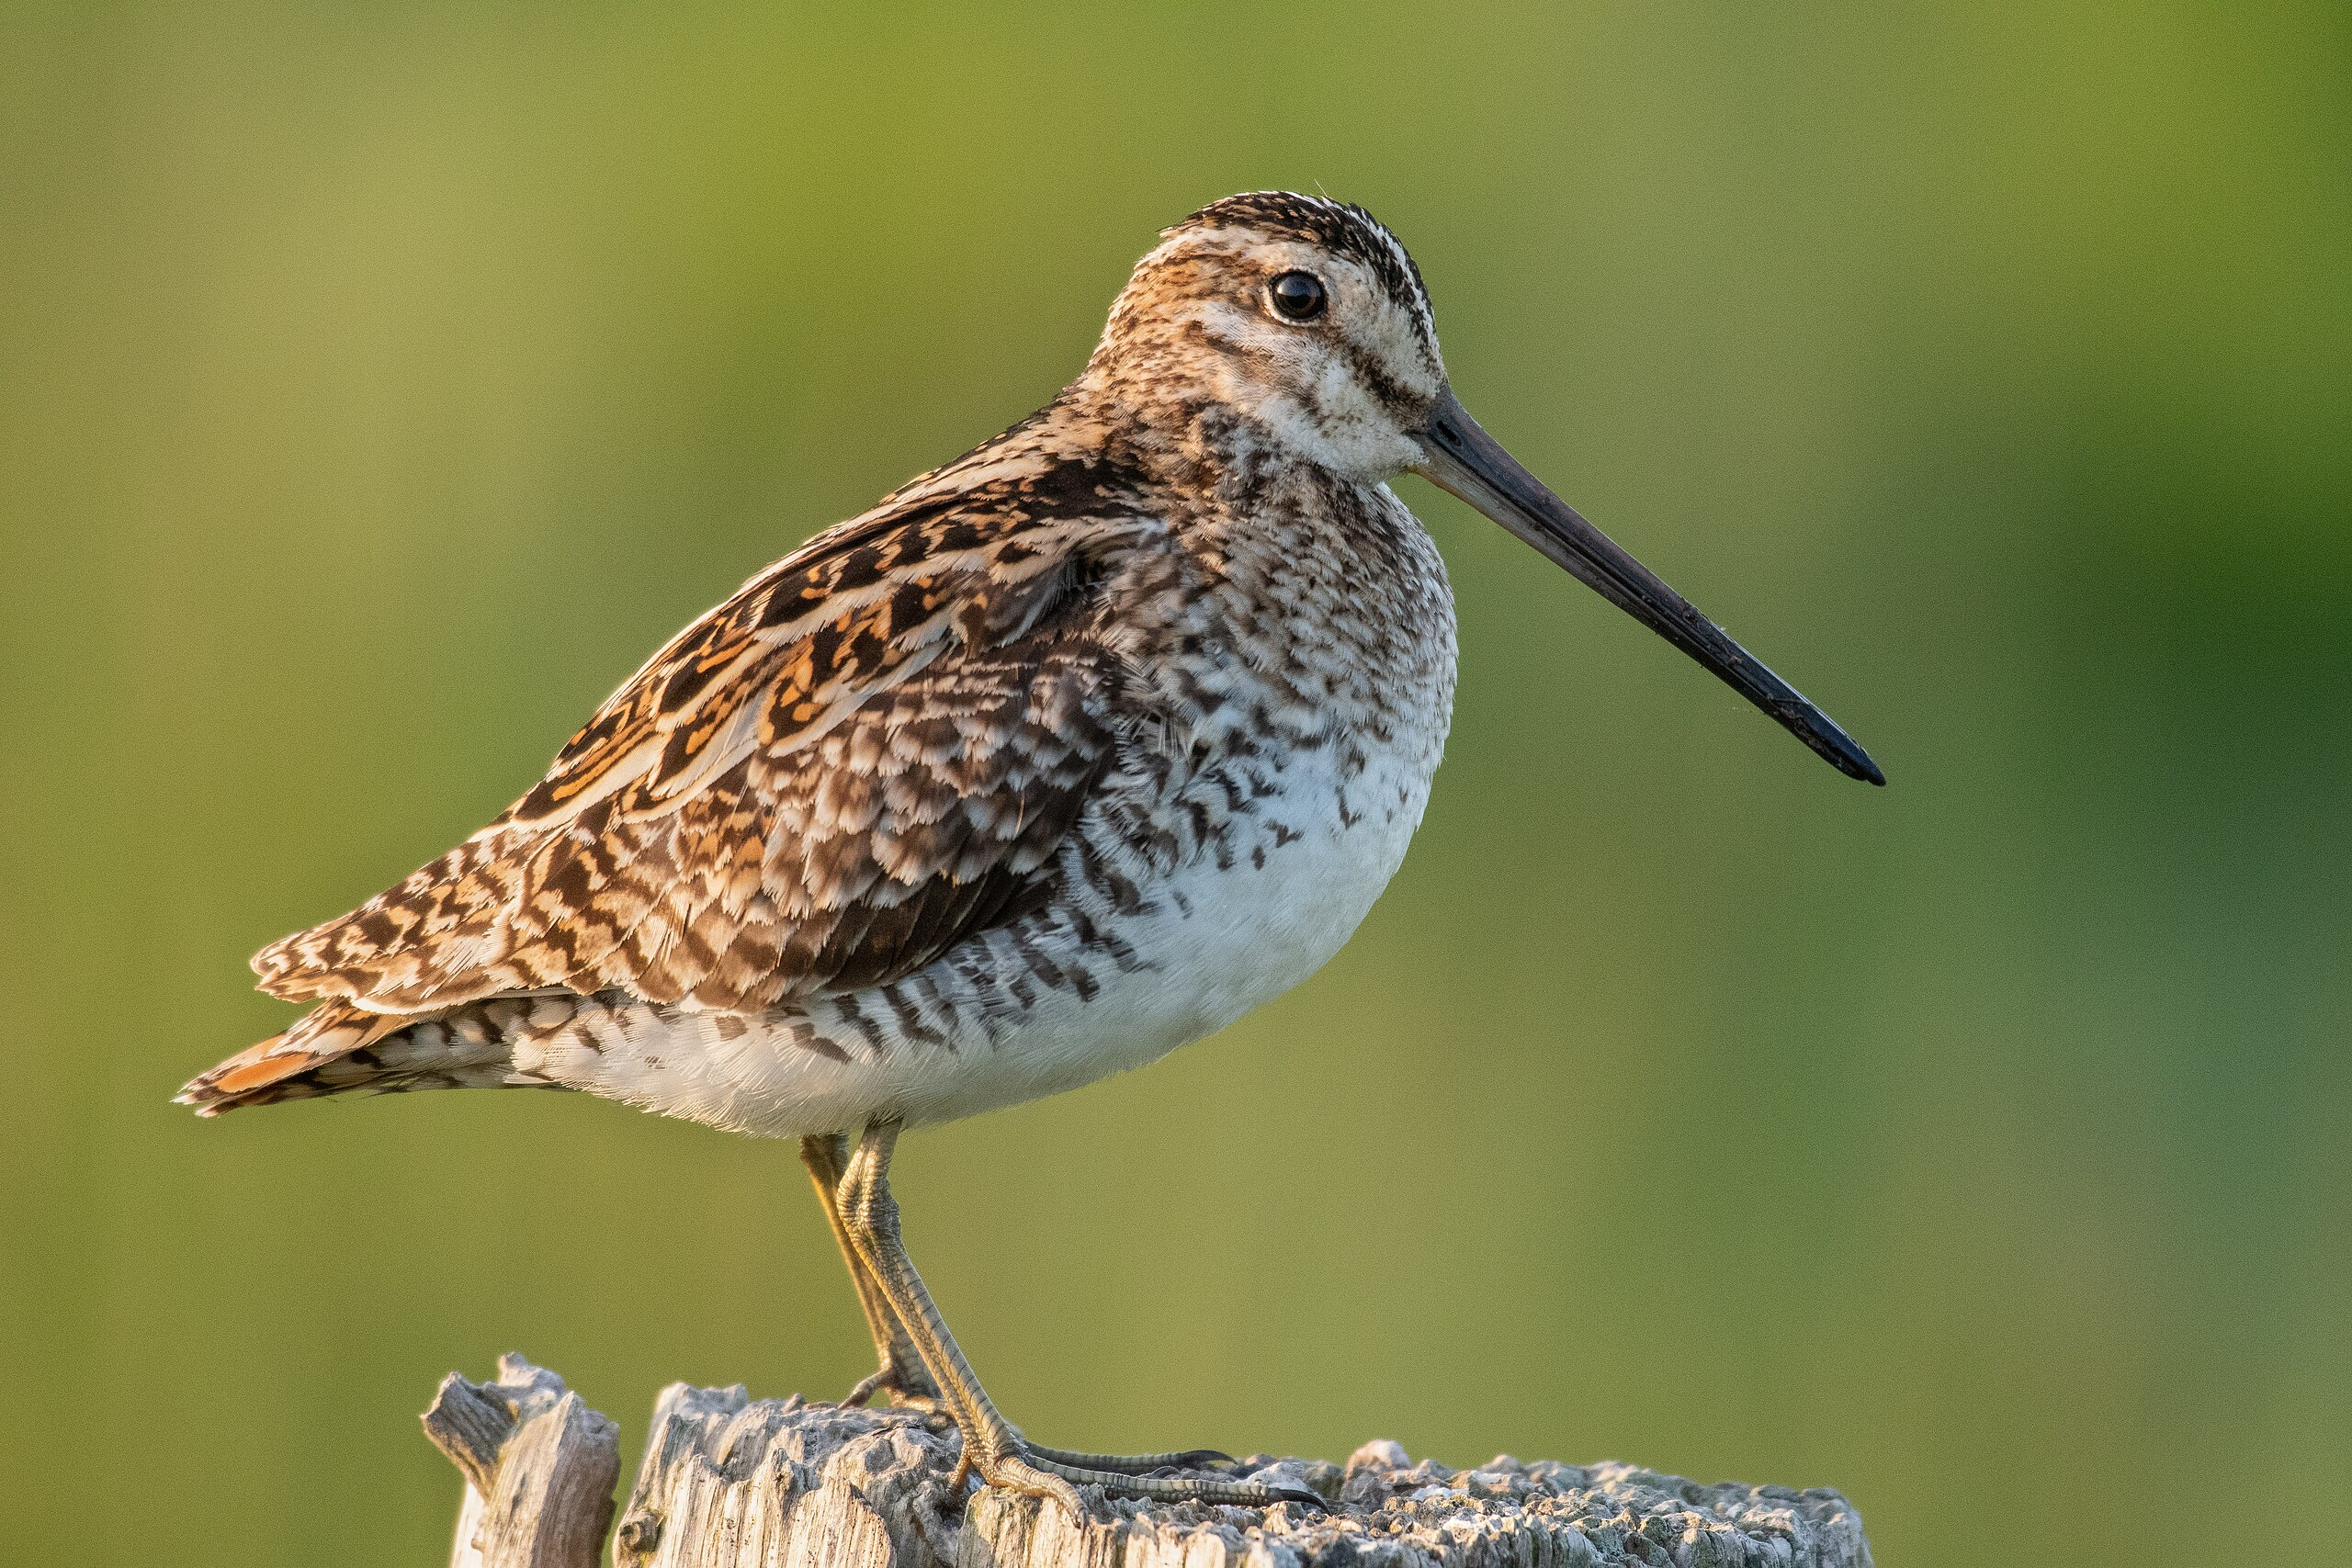
\includegraphics[width=0.8\linewidth, height=6.5cm, keepaspectratio]{Billeder/Dyr/Fugle/Vadefugle/dobbelt_bekksasin.jpg}%
\end{minipage}
}%
\end{columns}
\end{frame}
\begin{frame}{%
\begin{minipage}[t]{0.85\textwidth}
Enkeltbekkasin
\end{minipage}%
\hfill
\begin{minipage}[t]{0.1\textwidth}
\raggedleft

\includegraphics[width=0.55cm, height=0.55cm, keepaspectratio]{Billeder/Ikoner/star.png}%
\end{minipage}%
}
\vspace{0.25em}
\begin{columns}[T]
% --- Venstre kolonne: Tekst ---
\column{0.55\textwidth}
\setlength{\parskip}{0.5em}
\small
\RaggedRight\textbf{\textit{Lymnocryptes minimus}} – Ligner dobbeltbekkasin men er kun halv størrelse\par

\textbf{Udseende:} \\
\quad –  Gulige længdestriber, brun isse uden midterstribe. Kort næb kun lidt længere end hovedet.  

% --- Højre kolonne: Et billede ---
\column{0.40\textwidth}
\centering
\fbox{%
\begin{minipage}{\linewidth}
\centering
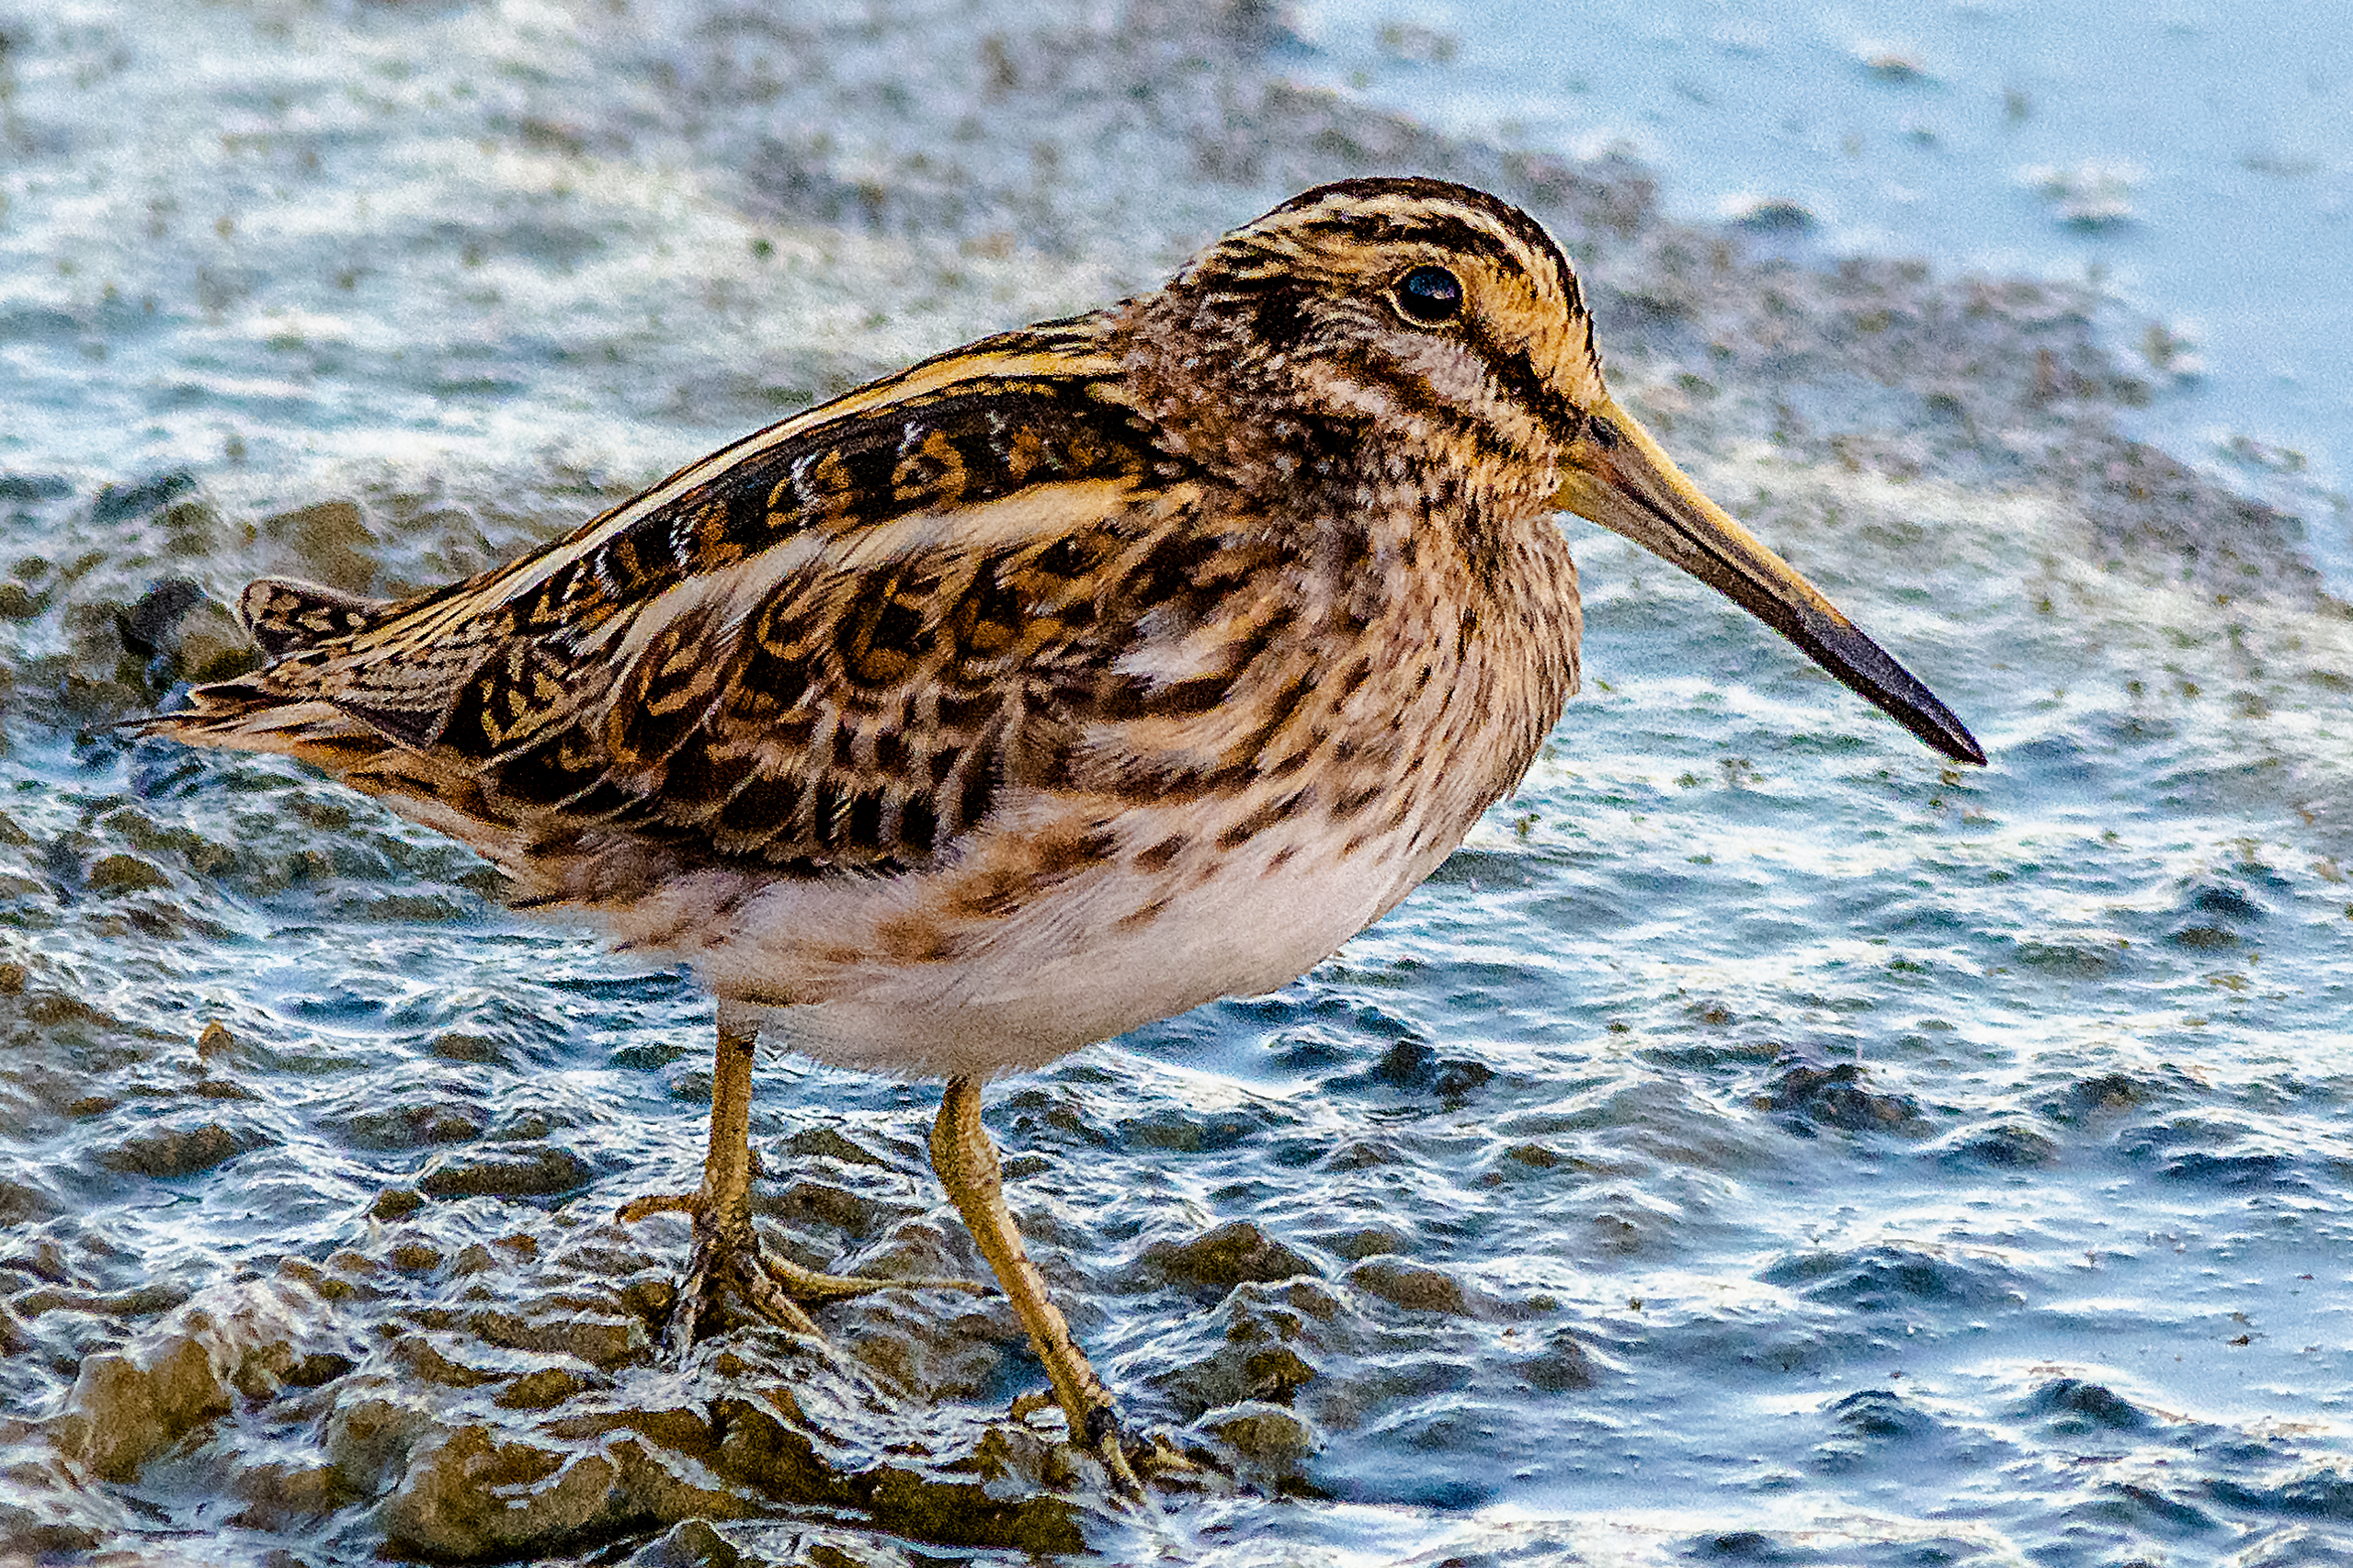
\includegraphics[width=0.8\linewidth, height=10cm, keepaspectratio]{Billeder/Dyr/Fugle/Vadefugle/enkelt_bekkasin.png}
\end{minipage}
}%
\end{columns}
\end{frame}
\begin{frame}{%
\begin{minipage}[t]{0.85\textwidth}
Skovsneppe
\end{minipage}%
\hfill
\begin{minipage}[t]{0.1\textwidth}
\raggedleft

\includegraphics[width=0.5cm, height=0.5cm, keepaspectratio]{Billeder/Ikoner/star.png}%
\hspace{0.2em}%

\includegraphics[width=0.5cm, height=0.5cm, keepaspectratio]{Billeder/Ikoner/star.png}
\end{minipage}%
}
\vspace{0.25em}
\begin{columns}[T]
% --- Venstre kolonne: Tekst ---
\column{0.55\textwidth}
\setlength{\parskip}{0.5em}
\small
\RaggedRight\textbf{\textit{Scolopax rusticola}} – Buttet og kraftig vadefugl med langt næb. Fineste jagttrofæ i Danmark\par 

\textbf{Udseende:} \\
\quad – Stort hoved med brede tværstriber på issen. Store øjne. Spraglet fjerdragt med brun, lysere og mørkere partier  \par

\textbf{Levesteder:} \\
\quad – Lever som eneste vadefugl i skove og læhegn

\textbf{Føde:} \\
\quad – Insekter, orme og snegle \par

\textbf{Udbredelse:} \\
\quad – Hele Danmark \par

\textbf{Træk/standfugl} \\
\quad – Begge \par

% --- Højre kolonne: Kun ét billede (Hannen) ---
\column{0.40\textwidth}
\centering
\fbox{%
\begin{minipage}{\linewidth}
\centering
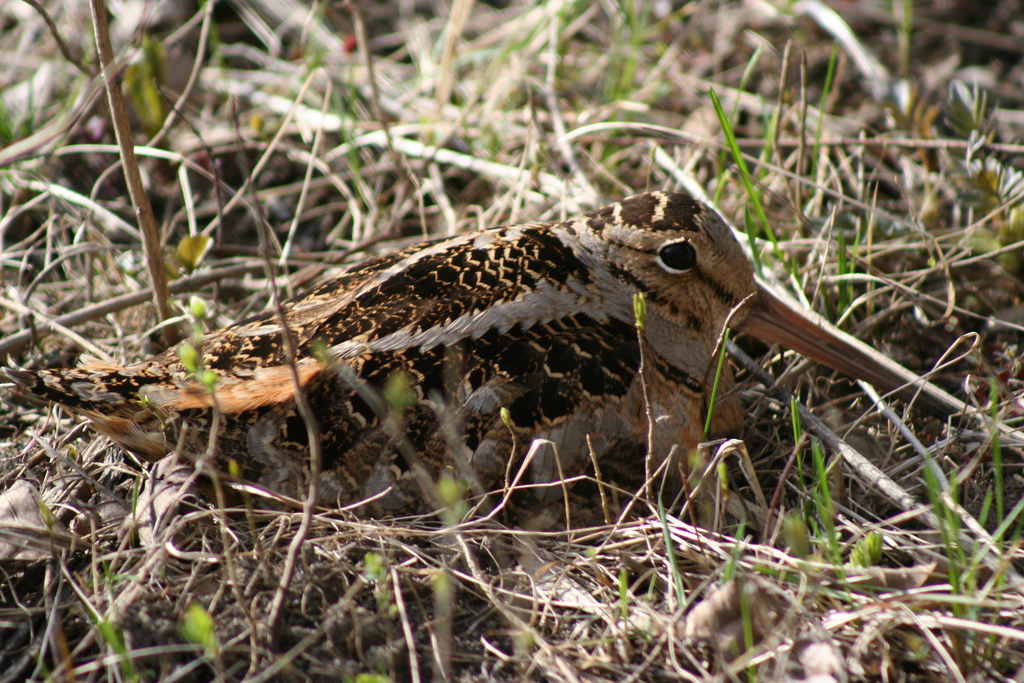
\includegraphics[width=0.8\linewidth, height=6.5cm, keepaspectratio]{Billeder/Dyr/Fugle/Vadefugle/skovsneppe.jpg}%
\end{minipage}
}%
\end{columns}
\end{frame}
\section{Fasanfugle (vildtkending og biologi)}

% ========== TITEL: FASANFUGLE ==========
\begin{frame}
  \vspace{1.5em}
  \begin{center}
    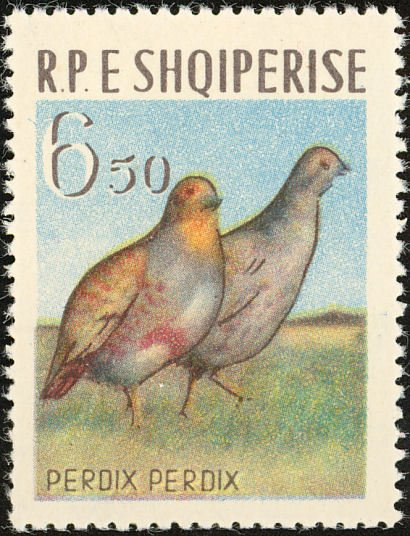
\includegraphics[width=12cm, height=4cm, keepaspectratio]{Billeder/Dyr/Fugle/Fasanfugle/fasanfugle.jpeg}\\[1.2em]
    {\LARGE \textbf{Fasanfugle}}
    \vspace{1em}
    \\ Artsbestemmelse og vildtbiologi
    \\[0.9em]
    {\tiny\color{gray}
    CC BY 4.0 – kan frit anvendes, også kommercielt. Rettighederne må ikke skærpes.\\[0.05em]
    Udviklet af Aleksander Sønder, OSJAGTTEGN.DK}
  \end{center}
\end{frame}

% ========== FASAN ==========
\begin{frame}{%
  \begin{minipage}[c]{0.30\textwidth}
    Fasan
  \end{minipage}%
  \hfill
  \begin{minipage}[c]{0.45\textwidth}
    \footnotesize
    \textbf{Jagttid:} 1.\ oktober -- 31.\ januar
  \end{minipage}%
  \hfill
  \begin{minipage}[c]{0.15\textwidth}
    \noindent\raggedleft
    
\includegraphics[width=0.5cm, height=0.5cm, keepaspectratio]{Billeder/Ikoner/star.png}%
    \hspace{0.2em}%
    
\includegraphics[width=0.5cm, height=0.5cm, keepaspectratio]{Billeder/Ikoner/star.png}%
    \hspace{0.2em}%
    
\includegraphics[width=0.5cm, height=0.5cm, keepaspectratio]{Billeder/Ikoner/star.png}
  \end{minipage}%
}
  \vspace{0.25em}
  \begin{columns}[T]
    % --- Venstre kolonne: Tekst ---
    \column{0.45\textwidth}
    \setlength{\parskip}{0.5em}
    \tiny
    \RaggedRight
    \textbf{\textit{Phasianus colchicus}} – stor hønsefugl med lang hale \par
    \textbf{Udseende:}\\
    \quad – Kok: Kobberrød krop, grønt hoved, røde kindpletter, ofte hvid halsring \\
    \quad – Høne: Brunspraglet, mere camoufleret, kortere hale \par
    \textbf{Levesteder:} Marker, læhegn, småskove og moser. \par
    \textbf{Føde:} Frø, korn, bær, insekter og snegle. \par
    \textbf{Udbredelse:} Hele Danmark. \par
    \textbf{Træk/standfugl:} Standfugl \par
    \textbf{Forplantning:}\\
    \quad – \textbf{Yngleforhold:} Yngler i hele Danmark \\
    \quad – \textbf{Kønsmoden:} Ca. 1 år \\
    \quad – \textbf{Mono/polygam:} Polygam \\
    \quad – \textbf{Bestandsomsætning:} Hurtig \\
    \quad – \textbf{Kuld:} 8–15 æg
    % --- Højre kolonne: To billeder ---
    \column{0.52\textwidth}
    \centering
    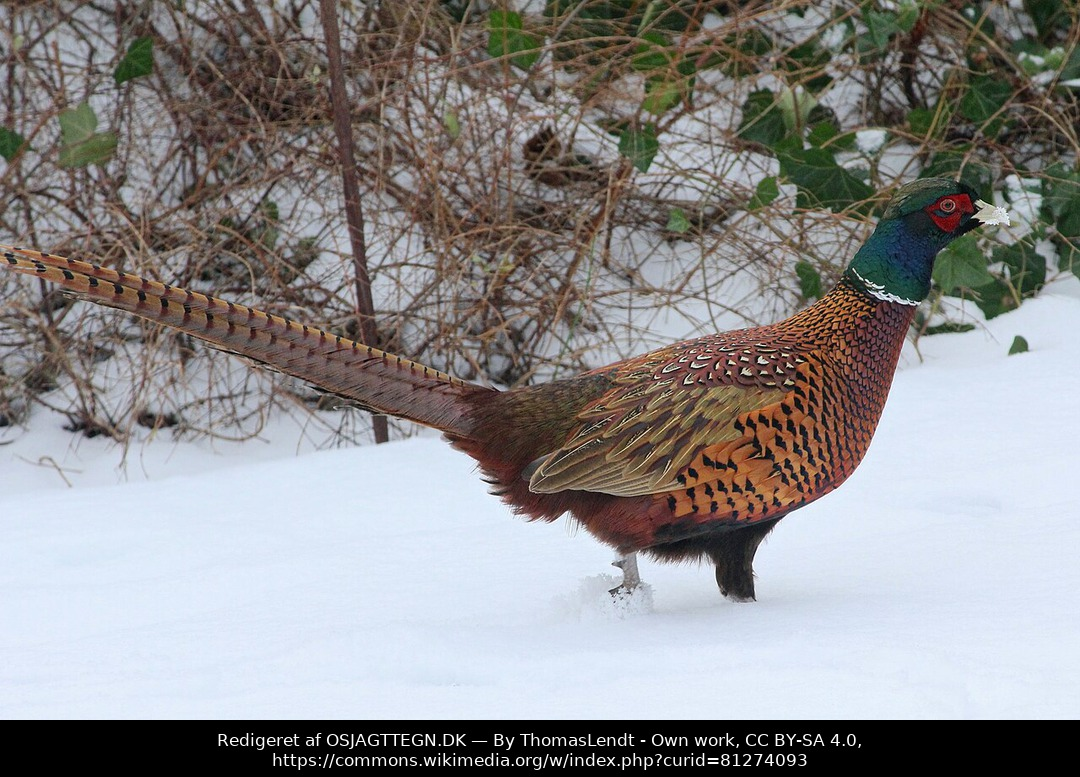
\includegraphics[width=0.92\linewidth, height=3cm, keepaspectratio]{Billeder/Dyr/Fugle/Fasanfugle/Fasan/fasan-male-01.jpg}\\[0.45em]
    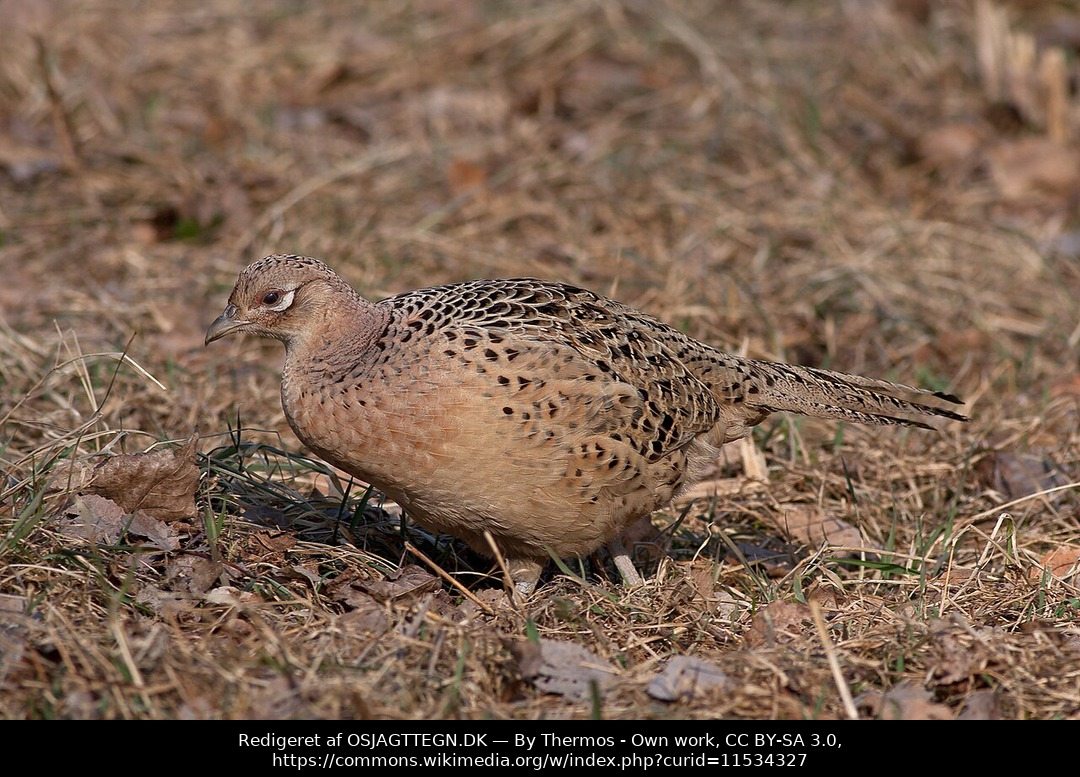
\includegraphics[width=0.92\linewidth, height=3cm, keepaspectratio]{Billeder/Dyr/Fugle/Fasanfugle/Fasan/fasan-female-01.jpg}\\[0.25em]
    \footnotesize Kok øverst, høne nederst
  \end{columns}
\end{frame}
% ========== AGERHØNE ==========
\begin{frame}{%
  \begin{minipage}[c]{0.30\textwidth}
    Agerhøne
  \end{minipage}%
  \hfill
  \begin{minipage}[c]{0.45\textwidth}
    \footnotesize
    \textbf{Jagttid:} 16.\ september -- 31.\ oktober*
  \end{minipage}%
  \hfill
  \begin{minipage}[c]{0.15\textwidth}
    \noindent\raggedleft
    
\includegraphics[width=0.5cm, height=0.5cm, keepaspectratio]{Billeder/Ikoner/star.png}%
    \hspace{0.2em}%
    
\includegraphics[width=0.5cm, height=0.5cm, keepaspectratio]{Billeder/Ikoner/star.png}%
    \hspace{0.2em}%
    
\includegraphics[width=0.5cm, height=0.5cm, keepaspectratio]{Billeder/Ikoner/star.png}
  \end{minipage}%
}
  \vspace{0.25em}
  \begin{columns}[T]
    % --- Venstre kolonne: Tekst ---
    \column{0.45\textwidth}
    \setlength{\parskip}{0.45em}
    \tiny
    \RaggedRight
    \textbf{\textit{Perdix perdix}} – lille, buttet hønsefugl med kort hale \par
    \textbf{Udseende:}\\
    \quad – Gråbrun med orangebrunt ansigt og rødbrun hale \\
    \quad – Han har typisk en større mørk hesteskoformet plet på bugen \par
    \textbf{Levesteder:} Åbent agerland med marker, læhegn, skel og enge. \par
    \textbf{Føde:} Ukrudtsfrø, korn og grønt. Kyllinger lever først af insekter. \par
    \textbf{Udbredelse:} Hele Danmark, men i tilbagegang. \par
    \textbf{Træk/standfugl:} Standfugl \par
    \textbf{Forplantning:}\\
    \quad – \textbf{Yngleforhold:} Yngler i hele Danmark \\
    \quad – \textbf{Kønsmoden:} Ca. 1 år \\
    \quad – \textbf{Mono/polygam:} Monogam \\
    \quad – \textbf{Bestandsomsætning:} Hurtig \\
    \quad – \textbf{Kuld:} 10–20 æg \par
    \textbf{*Bemærk:} Lokale jagttider, især vest for Storebælt.
    % --- Højre kolonne: Ét billede ---
    \column{0.52\textwidth}
    \centering
    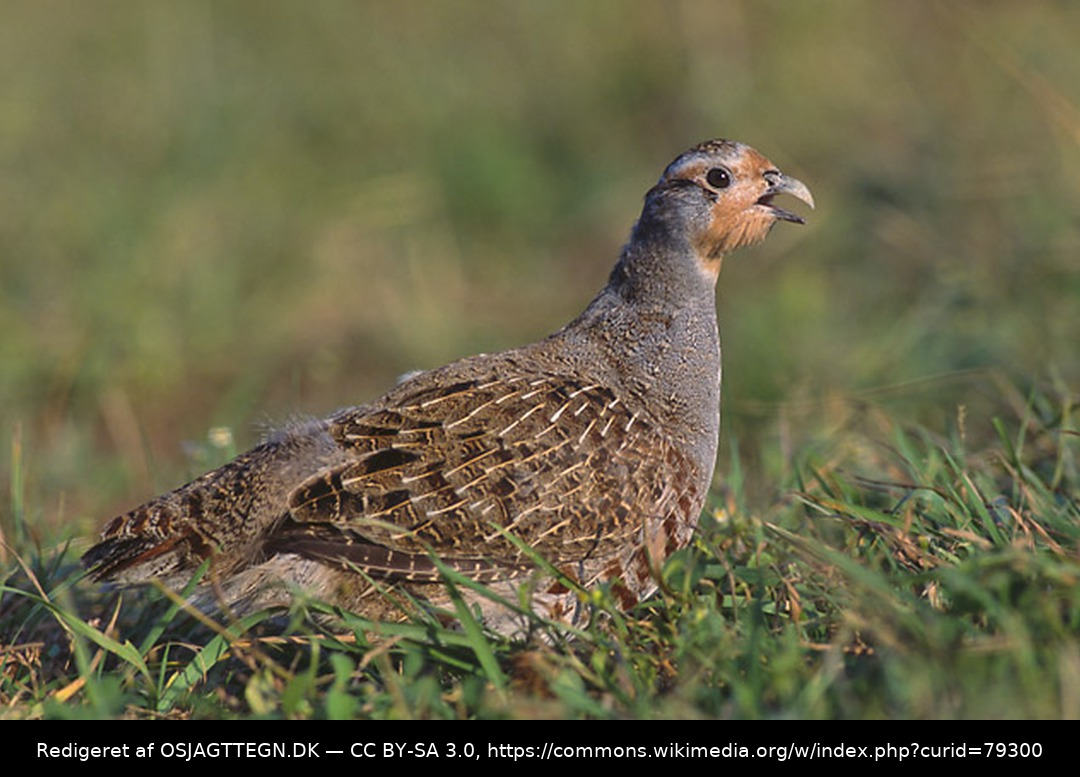
\includegraphics[width=\linewidth, height=7.2cm, keepaspectratio]{Billeder/Dyr/Fugle/Fasanfugle/Agerhøne/agerhoene-01.jpg}
  \end{columns}
\end{frame}
\section{Udsætning af vildt}

\begin{frame}
  \vspace{3em}
  \begin{center}
    {\LARGE \textbf{Udsætning af vildt}
    }
    \\
    \vspace{1em}
    Bekendtgørelse om udsætning af vildt, jagtmåder og jagtredskaber
    \\
    \vspace{1em}
    BEK nr 1652 af 19/12/2017, Kapitel 6
  \end{center}
\end{frame}

\begin{frame}{Generelt vedrørende udsætning af vildt}

\textbf{Hovedregel:} \\
Vildt må \textbf{ikke} udsættes i naturen uden tilladelse fra myndigheden.

\textbf{Undtagelse – kun disse tre arter må udsættes uden tilladelse:}
\begin{itemize}
    \item \textbf{Fasan} (Phasianus colchicus): 1. april – 31. august
    \item \textbf{Agerhøne} (Perdix perdix): 1. april – 15. august
    \item \textbf{Gråand} (Anas platyrhynchos): 1. april – 31. juli (i ferske vande)
\end{itemize}

\textbf{Vigtige fælleskrav for alle tre arter:}
\begin{itemize}
    \item \textbf{Alle} udsætninger skal indberettes digitalt senest 1 uge efter
    \item Udsætning af \textbf{mere end 100 fugle i alt} (fasan + agerhøne + gråand) kræver gennemført \textbf{godkendt kursus}
    \item Fravigelse fra basisreglerne (f.eks. højere tæthed end 1/ha for fasan/agerhøne) kræver \textbf{biotopplan}
\end{itemize}

\textbf{Alle andre vildtarter:} \\
Kræver særskilt tilladelse – udsætning er generelt forbudt.

\end{frame}




\begin{frame}{Udsætning af fasaner}

\begin{columns}[T] % T = top-aligned

\begin{column}{0.48\textwidth}
\textbf{Regler ved udsætning af fasaner:}
\begin{itemize}
    \item Kan udsættes 1. april til 31. august 
    \item Under 100ha max 100 fugle
    \item Over 100ha 1 fugl pr ha
    \item Biotopplan implementeret op til 7 fugle pr ha
    \item 5 årig biotopplan 2 år inde implementeret op til 12 fugle pr ha
    \item Afvigelser fra 1 fugle pr ha afhænger af pointsystem
    \item Alle udsætninger skal indberettes senest 1 uge efter udsætningen
\end{itemize}
\end{column}

\begin{column}{0.3\textwidth}
    % Vælg én af disse – de ser godt ud i præsentation
    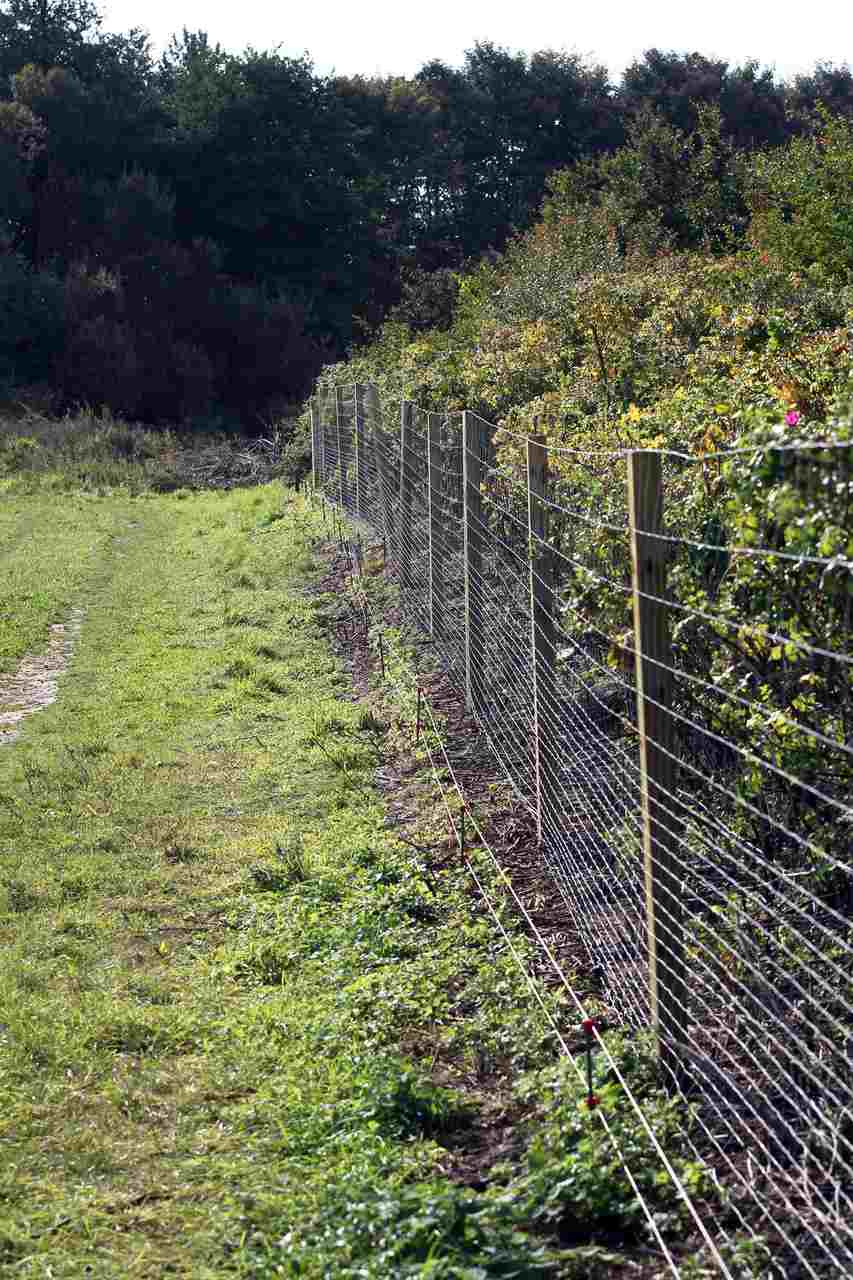
\includegraphics[width=\textwidth]{Billeder/Vildtforvaltning/udsætning/fasanvoilere.jpg}
    % Eller brug et af de gode eksempler:
    % \includegraphics[width=\textwidth]{vegetationsstriber_midtmark_ex.jpg}
\end{column}

\end{columns}

\end{frame}



\begin{frame}{Udsætning af agerhøns }

\begin{columns}[T] % T = top-aligned

\begin{column}{0.48\textwidth}
\textbf{Regler ved udsætning af agerhøns:}
\begin{itemize}
    \item Kan udsættes 1. april til 15. august
    \item Under 100 ha max 100 fugle
    \item Over 100 ha 1 fugl pr. ha
    \item Biotopplan implementeret op til 4 agerhøns pr. ha)
    \item 5-årig biotopplan 2 år inde implementeret op til max 4 agerhøns pr. ha
    \item Afvigelser fra 1 fugl pr. ha afhænger af pointsystem
    \item Alle udsætninger skal indberettes senest 1 uge efter udsætningen
\end{itemize}
\end{column}

\begin{column}{0.4\textwidth}
    % Godt billede af agerhøne eller biotop med agerhøns
    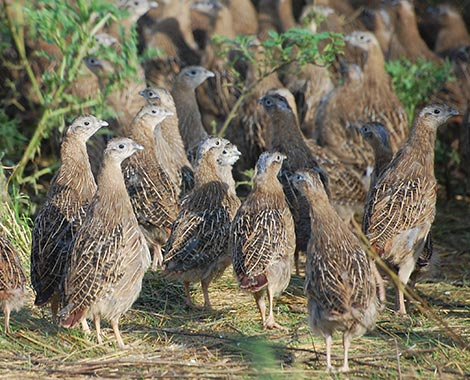
\includegraphics[width=\textwidth]{Billeder/Vildtforvaltning/udsætning/agerhøns.jpg}
    % Alternativer: agerhøne_i_mark.jpg eller vegetationsstriber_agerhoene.jpg
\end{column}

\end{columns}

\end{frame}




\begin{frame}{Udsætning af gråænder}

\begin{columns}[T] % T = top-aligned

\begin{column}{0.48\textwidth}
\textbf{Regler i ferske vande:}
\begin{itemize}
    \item Kan udsættes 1. april til 31. juli
    \item 1 ælling pr. 150 m² åben vandflade
    \item Eller 1 voksen and pr. 300 m² åben vandflade
    \item Ingen generel ha-begrænsning som ved fasan/agerhøne
    \item Ingen biotopplan-krav for højere antal
    \item Alle udsætninger skal indberettes senest 1 uge efter udsætningen
    \item Over 100 fugle (samlet med fasan/agerhøne) kræver godkendt kursus
\end{itemize}
\end{column}

\begin{column}{0.3\textwidth}
    % Vælg én af disse – de ser godt ud i præsentation
    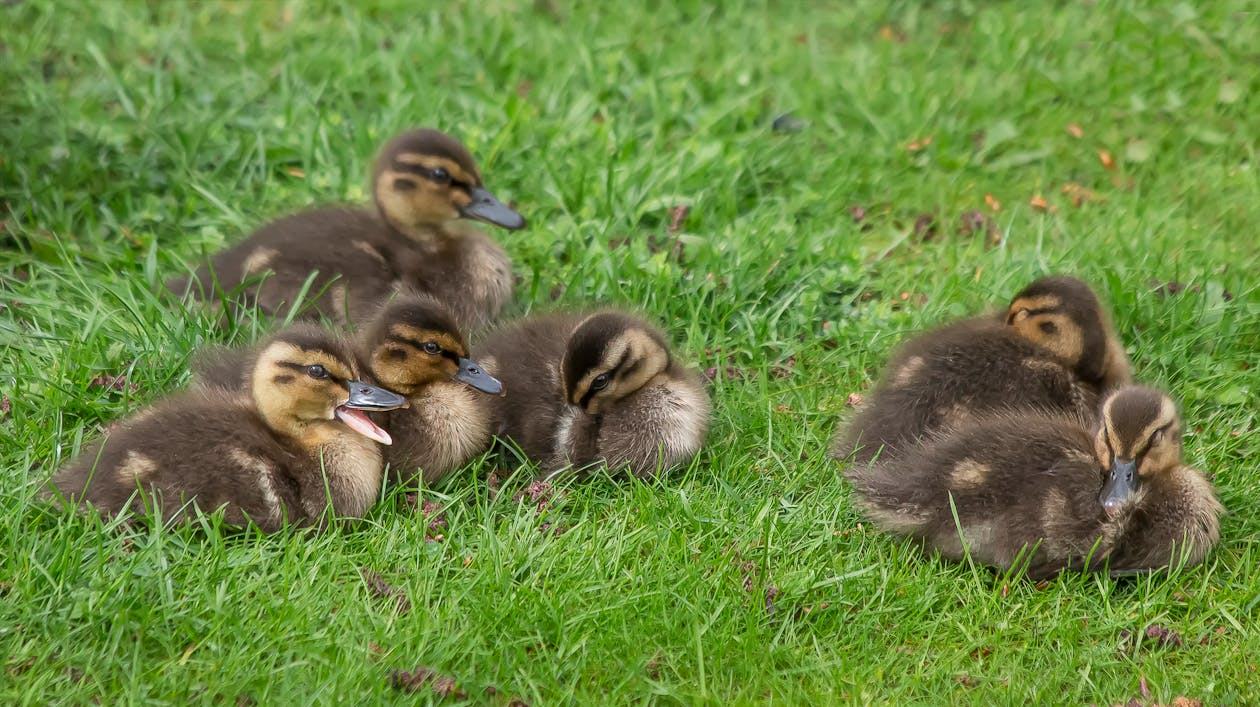
\includegraphics[width=\textwidth]{Billeder/Vildtforvaltning/udsætning/gråandeællinger.jpeg}
    % Eller brug et af de gode eksempler:
    % \includegraphics[width=\textwidth]{vegetationsstriber_midtmark_ex.jpg}
\end{column}

\end{columns}

\end{frame}
\section{Æggebekendtgørelsen}

\begin{frame}
  \vspace{3em}
  \begin{center}
    {\LARGE \textbf{"Æggebekendtgørelsen"}
    }
    \\
    \vspace{1em}
    Bekendtgørelse om æg fra vilde fugle og registrering af ægsamlinger
    \\
    \vspace{1em}
    BEK nr 936 af 27/06/2016, §§ 1 og 2
  \end{center}
\end{frame}


\begin{frame}{Bekendtgørelse om æg fra vilde fugle - Omfang (§ 1)}
\vspace{1em}

\small

\raggedright

\begin{itemize}

\itemsep0.6em % Justér afstand mellem bullets

\item Bekendtgørelsen omfatter æg fra vilde fugle, der er naturligt forekommende i den danske natur, samt æg fra arter omfattet af Fuglebeskyttelsesdirektivet (2009/147/EF) og underarter.

\item Gælder også tomme æg samt dele og produkter af æg.

\item Styrelsen for Vand- og Naturforvaltning afgør, om et æg er omfattet, og kan ved tvivl kræve anmeldelse/registrering.

\item Omfatter \textbf{ikke} æg fra landbrugsmæssigt opdræt af visse dyrearter.

\end{itemize}

\end{frame}



\begin{frame}{Bekendtgørelse om æg fra vilde fugle - Forbud og undtagelser (§ 2)}
\vspace{1em}

\small

\raggedright

\begin{itemize}

\itemsep0.6em % Justér afstand mellem bullets

\item Æg fra vilde fugle må \textbf{ikke} indsamles i naturen, opbevares, besiddes, modtages, købes, sælges, overdrages, udlånes, transporteres eller udstilles – medmindre anden lovgivning tillader det.

\item Undtagelser gælder for:
    \begin{itemize}
    \itemsep0.3em
    \item Indsamling af æg fra gråand i kunstige rugepladser
    \item Æg fra ødelagte reder af fasan, gråand eller agerhøne (til opdræt)
    \item Æg fra fasaner indfanget med særlig tilladelse fra styrelsen
    \end{itemize}

\item Den, der besidder æg fra fangenskabsopdrættede fugle af omfattede arter, skal kunne \textbf{godtgøre}, at æggene ikke stammer fra vilde fugle.

\end{itemize}

\end{frame}
\section{Måger (vildtkending og biologi)}

% ========== TITEL: MÅGEFUGLE ==========
\begin{frame}
  \vspace{1.5em}
  \begin{center}
    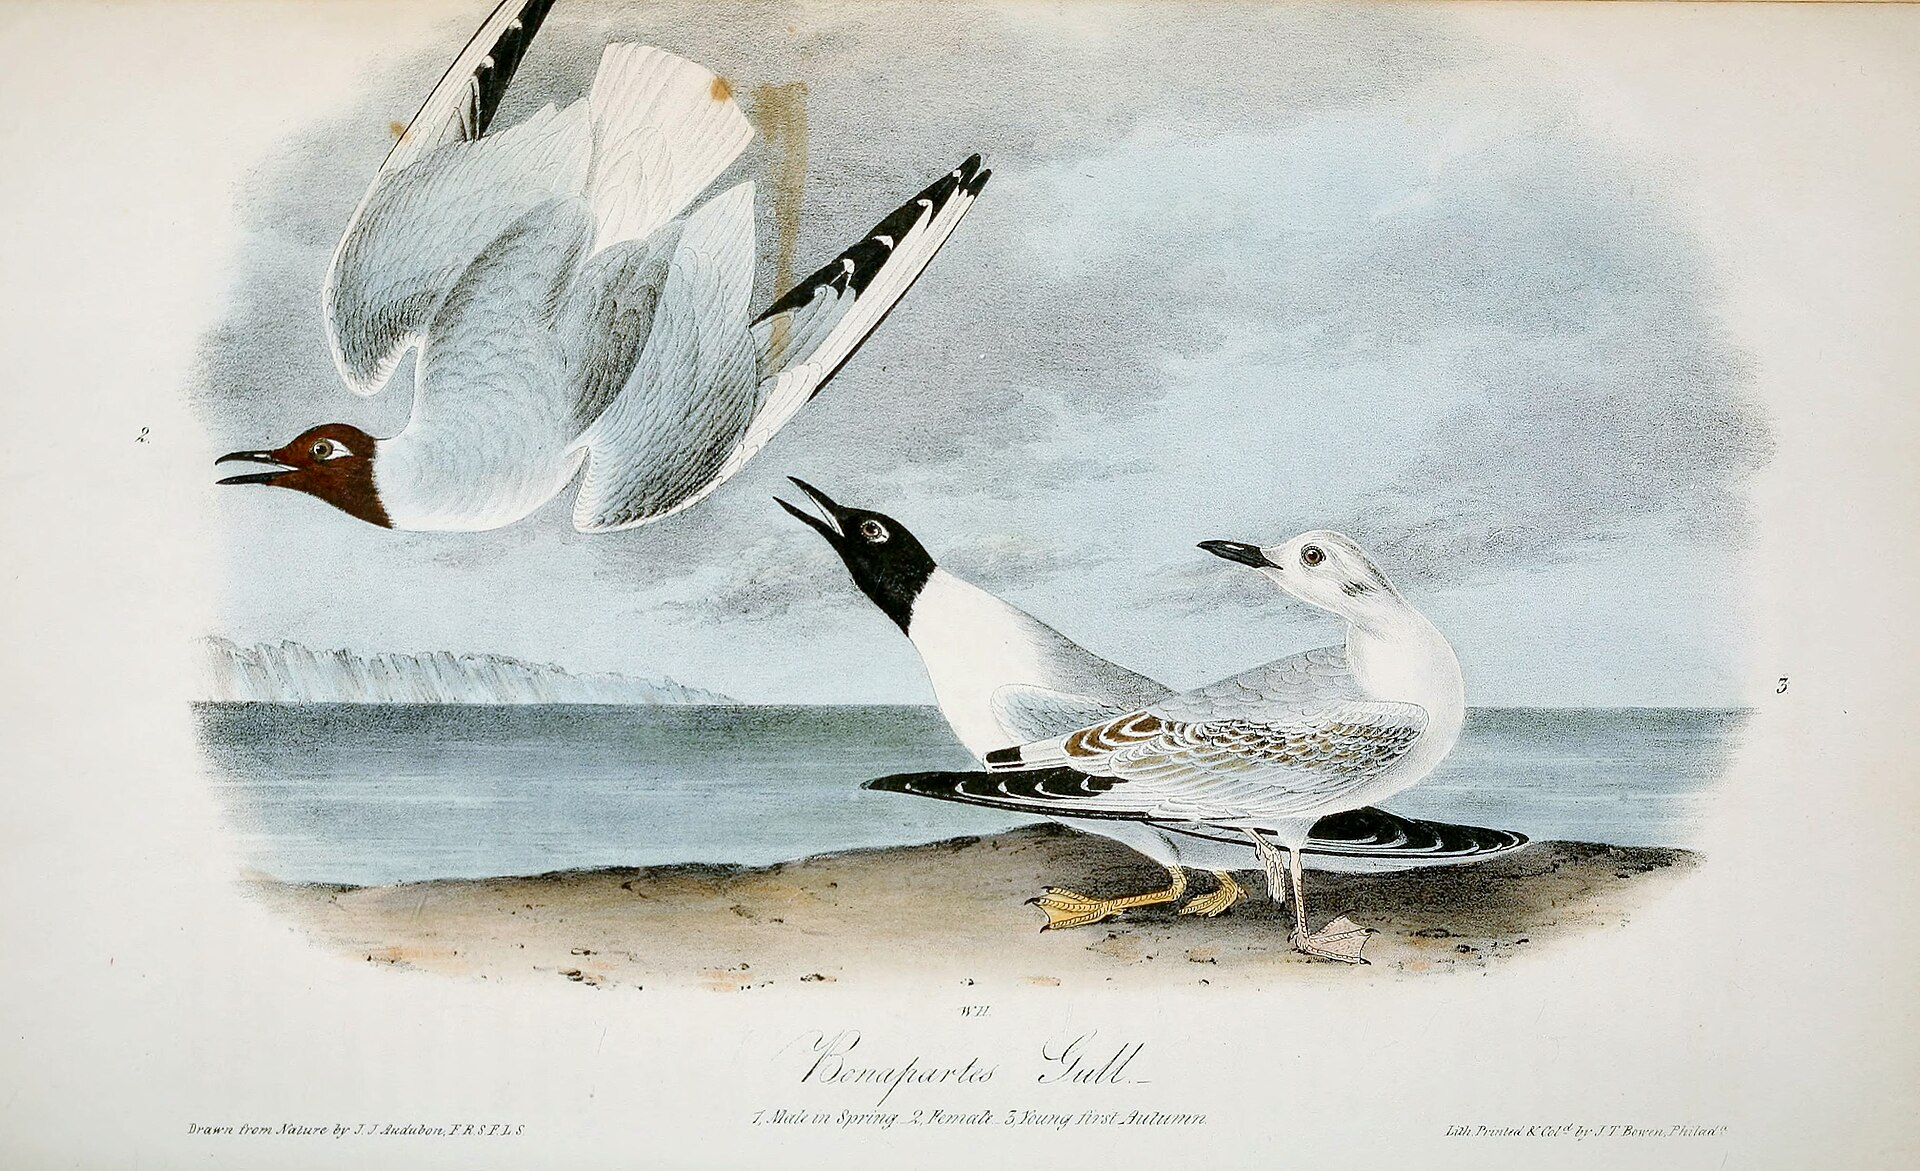
\includegraphics[width=12cm, height=4cm, keepaspectratio]{Billeder/Dyr/Fugle/Mågefugle/maagefugle.jpg}\\[1.2em]
    {\LARGE \textbf{Mågefugle}}\\[0.6em]
   
    Artsbestemmelse \& vildtbiologi\\[0.9em]
    {\tiny\color{gray}
    CC BY 4.0 – kan frit anvendes, også kommercielt. Rettighederne må ikke skærpes.\\[0.05em]
    Udviklet af Aleksander Sønder, OSJAGTTEGN.DK}
  \end{center}
\end{frame}



% ========== SØLVMÅGE ==========
\begin{frame}{%
  \begin{minipage}[c]{0.30\textwidth}
    Sølvmåge
  \end{minipage}%
  \hfill
  \begin{minipage}[c]{0.45\textwidth}
    \footnotesize
    \textbf{Jagttid:} 1.\ september -- 31.\ januar*
  \end{minipage}%
  \hfill
  \begin{minipage}[c]{0.15\textwidth}
    \noindent\raggedleft
    
\includegraphics[width=0.5cm, height=0.5cm, keepaspectratio]{Billeder/Ikoner/star.png}%
    \hspace{0.2em}%
    
\includegraphics[width=0.5cm, height=0.5cm, keepaspectratio]{Billeder/Ikoner/star.png}
  \end{minipage}%
}
  \vspace{0.25em}
  \begin{columns}[T]
    \column{0.45\textwidth}
    \setlength{\parskip}{0.5em}
    \tiny
    \RaggedRight
    \textbf{\textit{Larus argentatus}} – stor og kraftig måge med flad isse \par
    \textbf{Udseende:}\\
    \quad – Grå ryg og vinger med sort vingespids \\
    \quad – Lyserøde ben \\
    \quad – Gult næb med rød plet på undernæbbets spids \par
    \textbf{Levesteder:} Ses overalt, hvor der er føde. \par
    \textbf{Føde:} Altædende. \par
    \textbf{Udbredelse:} Hele Danmark. \par
    \textbf{Træk/standfugl:} Standfugl \par
    \textbf{*Bemærk:} I flere østdanske kommuner først fra 1.\ november.
    \column{0.52\textwidth}
    \centering
    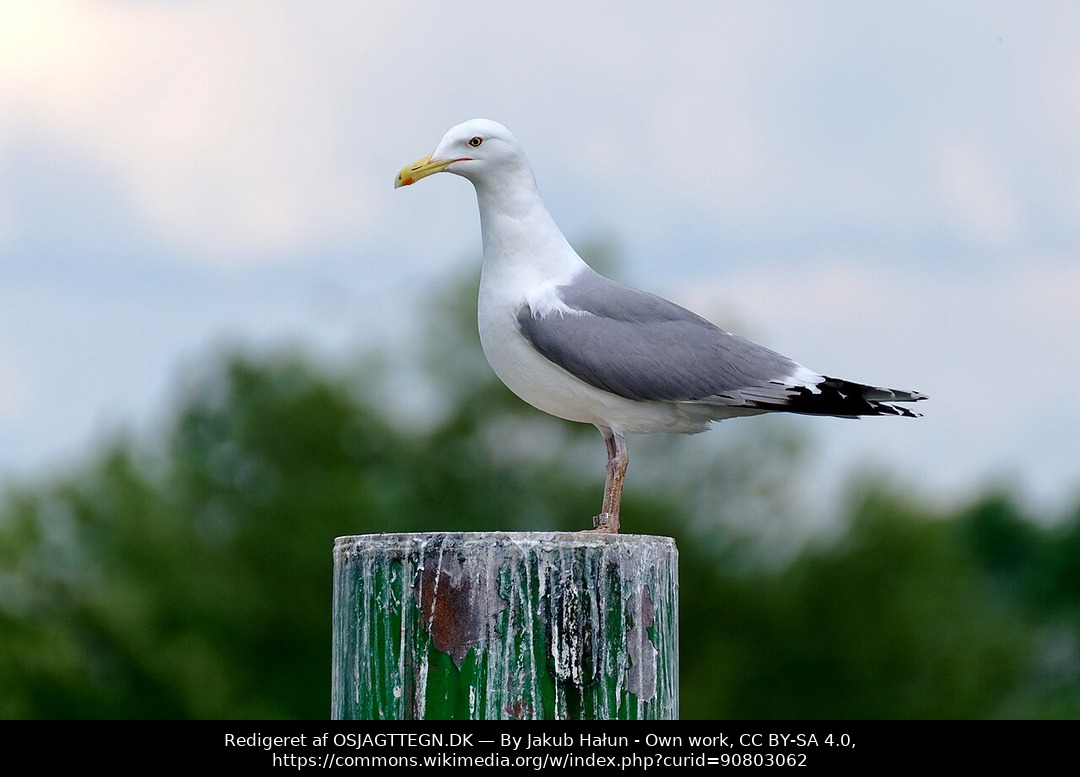
\includegraphics[width=\linewidth, height=7.2cm, keepaspectratio]{Billeder/Dyr/Fugle/Mågefugle/sølvmåge/soelvmaage-01.jpg}
  \end{columns}
\end{frame}
% ========== HÆTTEMÅGE (SOMMERDRAGT) ==========
\begin{frame}{%
  \begin{minipage}[c]{0.30\textwidth}
    Hættemåge\\[-0.1em]
    {\footnotesize (Sommerdragt)}
  \end{minipage}%
  \hfill
  \begin{minipage}[c]{0.45\textwidth}
    \footnotesize
    \textbf{Jagttid:} Ingen jagttid
  \end{minipage}%
  \hfill
  \begin{minipage}[c]{0.15\textwidth}
    \noindent\raggedleft
    
\includegraphics[width=0.5cm, height=0.5cm, keepaspectratio]{Billeder/Ikoner/star.png}
  \end{minipage}%
}
  \vspace{0.25em}
  \begin{columns}[T]
    \column{0.45\textwidth}
    \setlength{\parskip}{0.5em}
    \tiny
    \RaggedRight
    \textbf{\textit{Chroicocephalus ridibundus}} – lille, slank måge med hvidlig vingeforkant \par
    \textbf{Udseende:}\\
    \quad – Mørkebrun hætte som ikke går ned i nakken \\
    \quad – Rødt næb og røde ben \\
    \quad – Hvid krop med grå overside
    \column{0.52\textwidth}
    \centering
    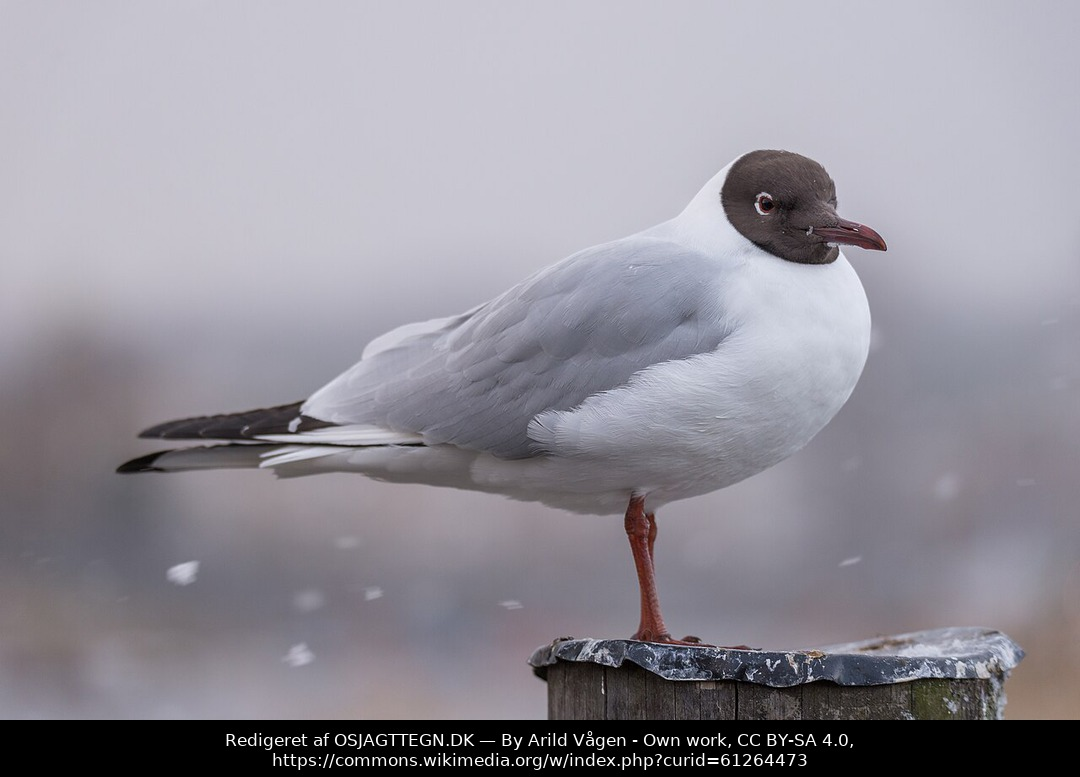
\includegraphics[width=\linewidth, height=7.2cm, keepaspectratio]{Billeder/Dyr/Fugle/Mågefugle/hættemåge/sommer.jpg}
  \end{columns}
\end{frame}

% ========== HÆTTEMÅGE (VINTERDRAGT) ==========
\begin{frame}{%
  \begin{minipage}[c]{0.30\textwidth}
    Hættemåge\\[-0.1em]
    {\footnotesize(Vinterdragt)}
  \end{minipage}%
  \hfill
  \begin{minipage}[c]{0.45\textwidth}
    \footnotesize
    \textbf{Jagttid:} Ingen jagttid
  \end{minipage}%
  \hfill
  \begin{minipage}[c]{0.15\textwidth}
    \noindent\raggedleft
    
\includegraphics[width=0.5cm, height=0.5cm, keepaspectratio]{Billeder/Ikoner/star.png}
  \end{minipage}%
}
  \vspace{0.25em}
  \begin{columns}[T]
    \column{0.45\textwidth}
    \setlength{\parskip}{0.5em}
    \tiny
    \RaggedRight
    \textbf{\textit{Chroicocephalus ridibundus}} – lille, slank måge med hvidlig vingeforkant \par
    \textbf{Udseende:}\\
    \quad – Ingen mørk hætte \\
    \quad – Mørkebrun plet bag øjet \\
    \quad – Hvidt hoved og hvid krop med grå overside
    \column{0.52\textwidth}
    \centering
    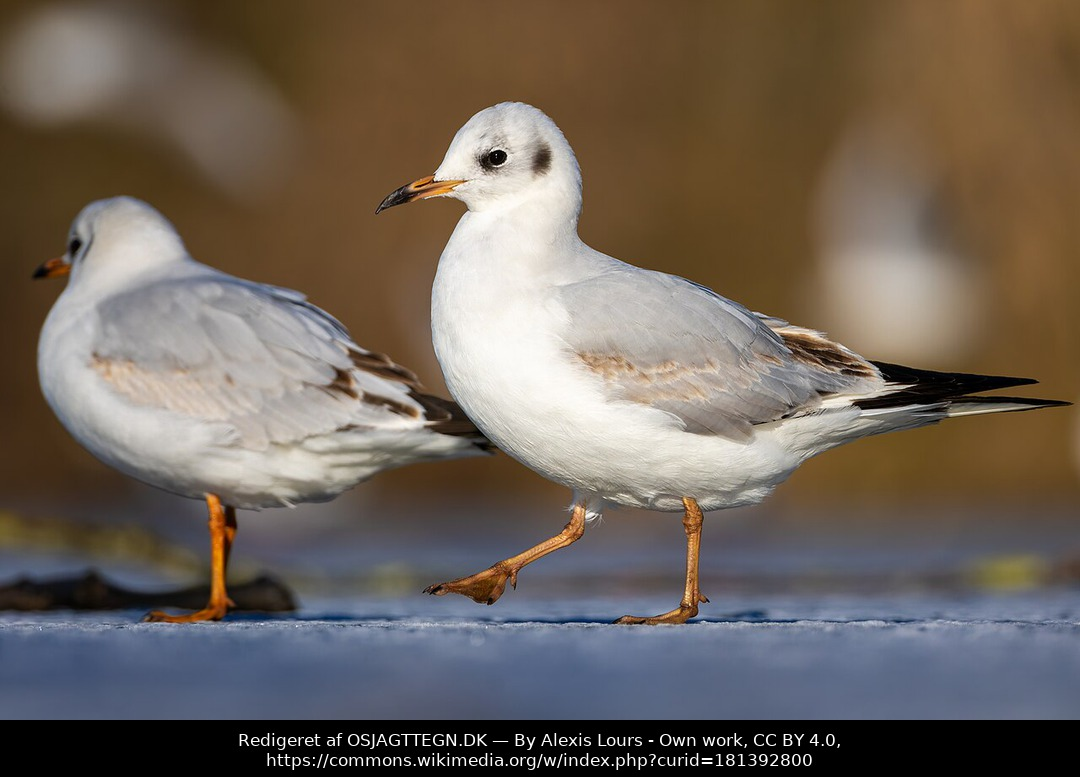
\includegraphics[width=\linewidth, height=7.2cm, keepaspectratio]{Billeder/Dyr/Fugle/Mågefugle/hættemåge/vinter.jpg}
  \end{columns}
\end{frame}
% ========== SILDEMÅGE ==========
\begin{frame}{%
  \begin{minipage}[c]{0.30\textwidth}
    Sildemåge
  \end{minipage}%
  \hfill
  \begin{minipage}[c]{0.45\textwidth}
    \footnotesize
    \textbf{Jagttid:} Ingen jagttid
  \end{minipage}%
  \hfill
  \begin{minipage}[c]{0.15\textwidth}
    \noindent\raggedleft
    
\includegraphics[width=0.5cm, height=0.5cm, keepaspectratio]{Billeder/Ikoner/star.png}
  \end{minipage}%
}
  \vspace{0.25em}
  \begin{columns}[T]
    \column{0.45\textwidth}
    \setlength{\parskip}{0.5em}
    \tiny
    \RaggedRight
    \textbf{\textit{Larus fuscus}} – mellemstor måge der ligner lille svartbag \par
    \textbf{Udseende:}\\
    \quad – Sort/mørk ryg og overvinger \\
    \quad – Hvide pletter på halefjerene \\
    \quad – Gule ben
    \column{0.52\textwidth}
    \centering
    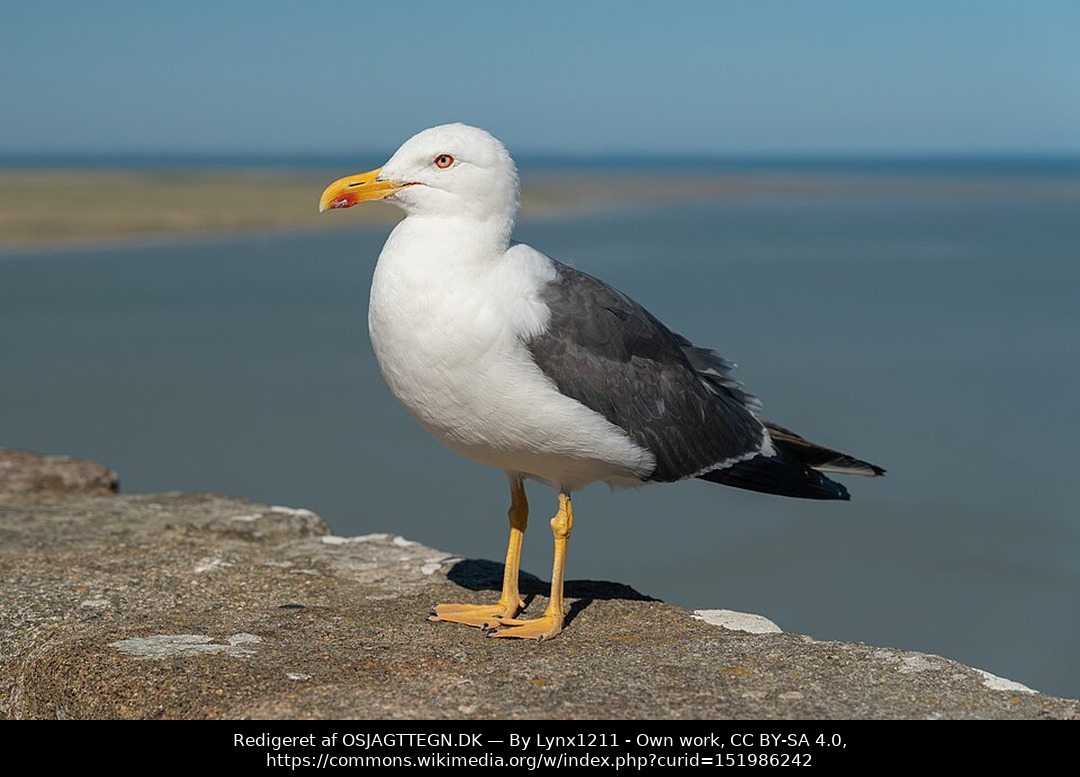
\includegraphics[width=\linewidth, height=7.2cm, keepaspectratio]{Billeder/Dyr/Fugle/Mågefugle/sildemåge/sildemaage-01.jpg}
  \end{columns}
\end{frame}
% ========== STORMMÅGE ==========
\begin{frame}{%
  \begin{minipage}[c]{0.30\textwidth}
    Stormmåge
  \end{minipage}%
  \hfill
  \begin{minipage}[c]{0.45\textwidth}
    \footnotesize
    \textbf{Jagttid:} Ingen jagttid
  \end{minipage}%
  \hfill
  \begin{minipage}[c]{0.15\textwidth}
    \noindent\raggedleft
    
\includegraphics[width=0.5cm, height=0.5cm, keepaspectratio]{Billeder/Ikoner/star.png}
  \end{minipage}%
}
  \vspace{0.25em}
  \begin{columns}[T]
    \column{0.45\textwidth}
    \setlength{\parskip}{0.5em}
    \tiny
    \RaggedRight
    \textbf{\textit{Larus canus}} – lille til mellemstor måge \par
    \textbf{Udseende:}\\
    \quad – Rundt hoved \\
    \quad – Mørkt øje (ser venlig ud) \\
    \quad – Slankt næb
    \column{0.52\textwidth}
    \centering
    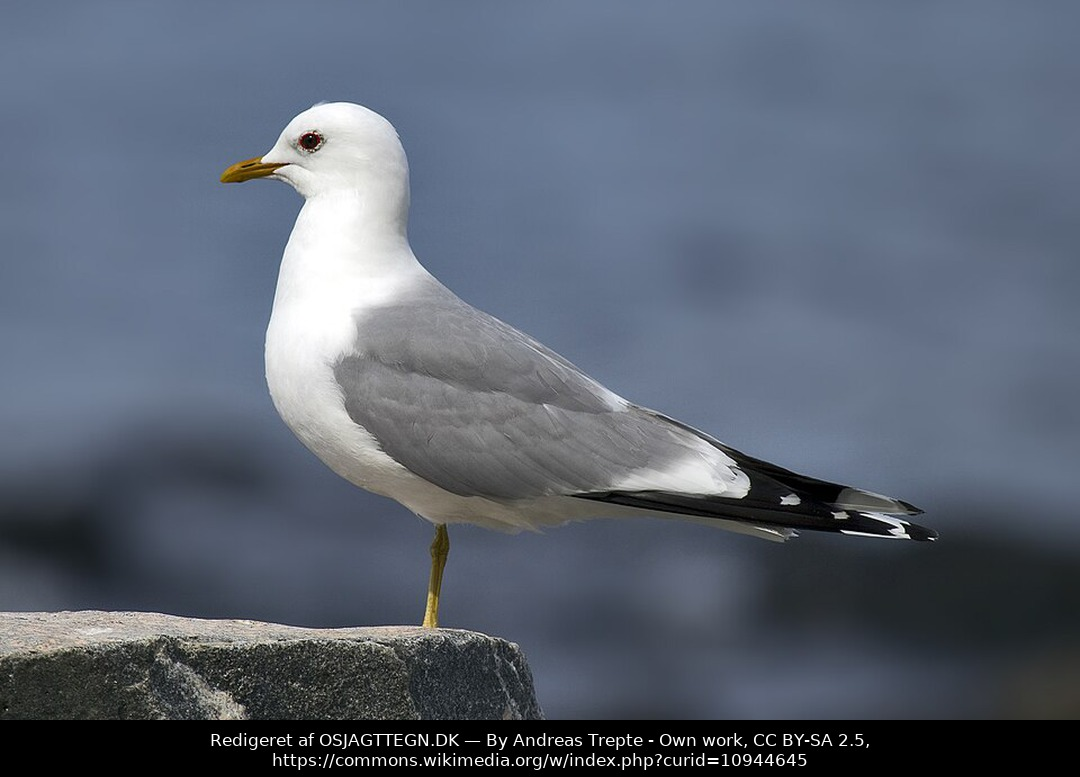
\includegraphics[width=\linewidth, height=7.2cm, keepaspectratio]{Billeder/Dyr/Fugle/Mågefugle/stormmåge/stormmaage-05.jpg}
  \end{columns}
\end{frame}
% ========== SVARTBAG ==========
\begin{frame}{%
  \begin{minipage}[c]{0.30\textwidth}
    Svartbag
  \end{minipage}%
  \hfill
  \begin{minipage}[c]{0.45\textwidth}
    \footnotesize
    \textbf{Jagttid:} Ingen jagttid
  \end{minipage}%
  \hfill
  \begin{minipage}[c]{0.15\textwidth}
    \noindent\raggedleft
    
\includegraphics[width=0.5cm, height=0.5cm, keepaspectratio]{Billeder/Ikoner/star.png}
  \end{minipage}%
}
  \vspace{0.25em}
  \begin{columns}[T]
    \column{0.45\textwidth}
    \setlength{\parskip}{0.5em}
    \tiny
    \RaggedRight
    \textbf{\textit{Larus marinus}} – meget stor og kraftig måge \par
    \textbf{Udseende:}\\
    \quad – Sort ryg og vingeoversider \\
    \quad – Hvide pletter på halen (blinklys) \\
    \quad – Lyserøde ben \\
    \quad – Kraftigt, ``fortrykket'' næb
    \column{0.52\textwidth}
    \centering
    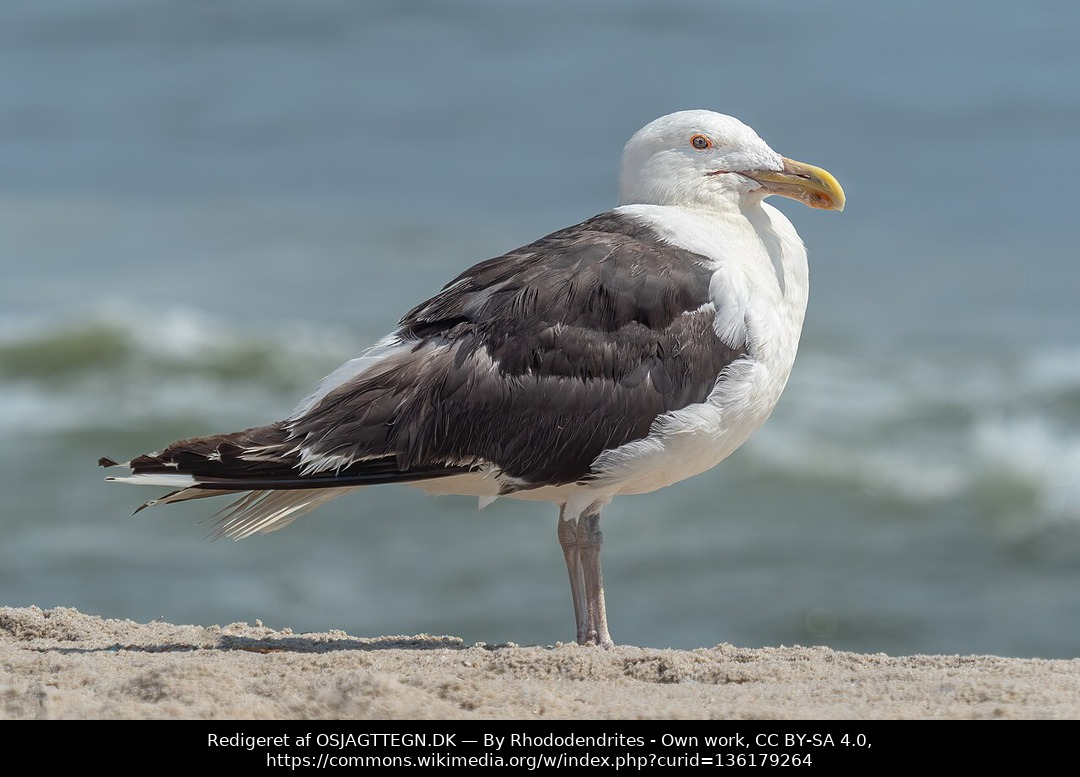
\includegraphics[width=\linewidth, height=7.2cm, keepaspectratio]{Billeder/Dyr/Fugle/Mågefugle/svartbag/svartbag-01.jpg}
  \end{columns}
\end{frame}
\begin{frame}
  \vspace{1.8em}
  \begin{center}
    \begin{minipage}{0.22\textwidth}
      \centering
      
\includegraphics[width=\linewidth]{Billeder/Dyr/Fugle/Mågefugle/qr/maagefugle_qr.png}
    \end{minipage}%
    \hspace{0.8em}%
    \begin{minipage}{0.62\textwidth}
      \raggedright
      \Large
      \textbf{Træning i artsbestemmelse af mågefugle}\\[0.35em]
      {\large https://osjagttegn.dk/maagefugle}
    \end{minipage}
  \end{center}
\end{frame}
\section{Vandhøns (vildtkending og biologi)}

% ========== TITEL: VANDHØNS ==========
\begin{frame}
  \vspace{1.5em}
  \begin{center}
    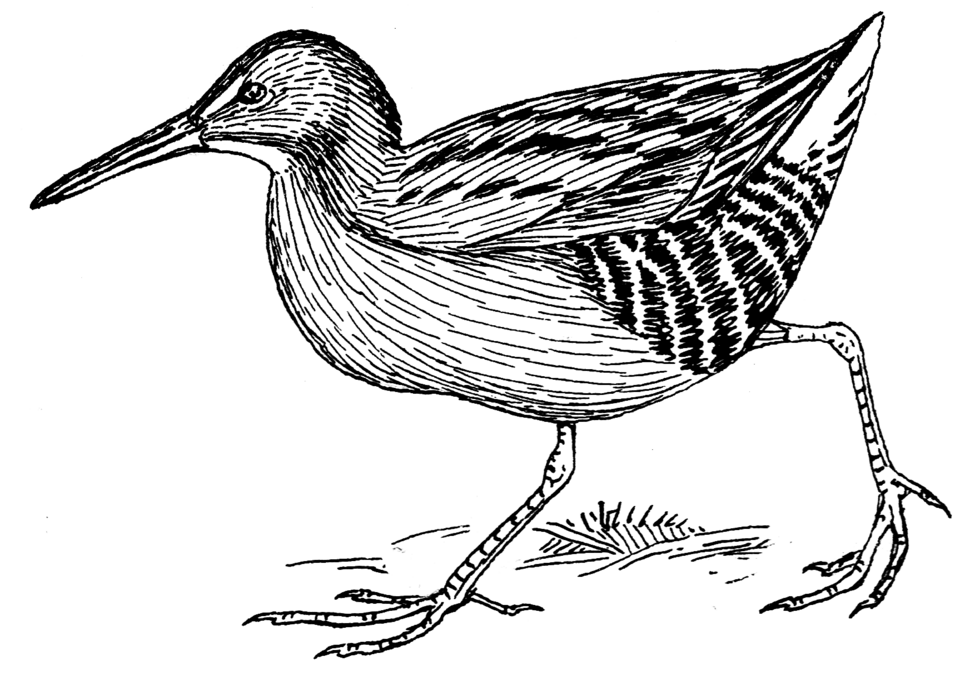
\includegraphics[width=12cm, height=4cm, keepaspectratio]{Billeder/Dyr/Fugle/Vandhøns/vandhøns.png}\\[1.2em]
    {\LARGE \textbf{Vandhøns}}\\[0.6em]
   
    Artsbestemmelse \& vildtbiologi\\[0.9em]
    {\tiny\color{gray}
    CC BY 4.0 – kan frit anvendes, også kommercielt. Rettighederne må ikke skærpes.\\[0.05em]
    Udviklet af Aleksander Sønder, OSJAGTTEGN.DK}
  \end{center}
\end{frame}

% ========== BLISHØNE ==========
\begin{frame}{%
  \begin{minipage}[c]{0.30\textwidth}
    Blishøne
  \end{minipage}%
  \hfill
  \begin{minipage}[c]{0.45\textwidth}
    \footnotesize
    \textbf{Jagttid:} 1.\ oktober -- 31.\ januar
  \end{minipage}%
  \hfill
  \begin{minipage}[c]{0.15\textwidth}
    \noindent\raggedleft
    
\includegraphics[width=0.5cm, height=0.5cm, keepaspectratio]{Billeder/Ikoner/star.png}%
    \hspace{0.2em}%
    
\includegraphics[width=0.5cm, height=0.5cm, keepaspectratio]{Billeder/Ikoner/star.png}
  \end{minipage}%
}
  \vspace{0.25em}
  \begin{columns}[T]
    \column{0.45\textwidth}
    \setlength{\parskip}{0.5em}
    \tiny
    \RaggedRight
    \textbf{\textit{Fulica atra}} – kraftig vandfugl med rund, skifersort krop og lange ben \par
    \textbf{Udseende:}\\
    \quad – Sort fjerdragt \\
    \quad – Hvid pandeblis \\
    \quad – Næb med rosa spids \par
    \textbf{Levesteder:} Søer og indre farvande. \par
    \textbf{Føde:} Vandplanter suppleret med muslinger, insekter og bløddyr. \par
    \textbf{Udbredelse:} Hele Danmark. \par
    \textbf{Træk/standfugl:} Begge
    \column{0.52\textwidth}
    \centering
    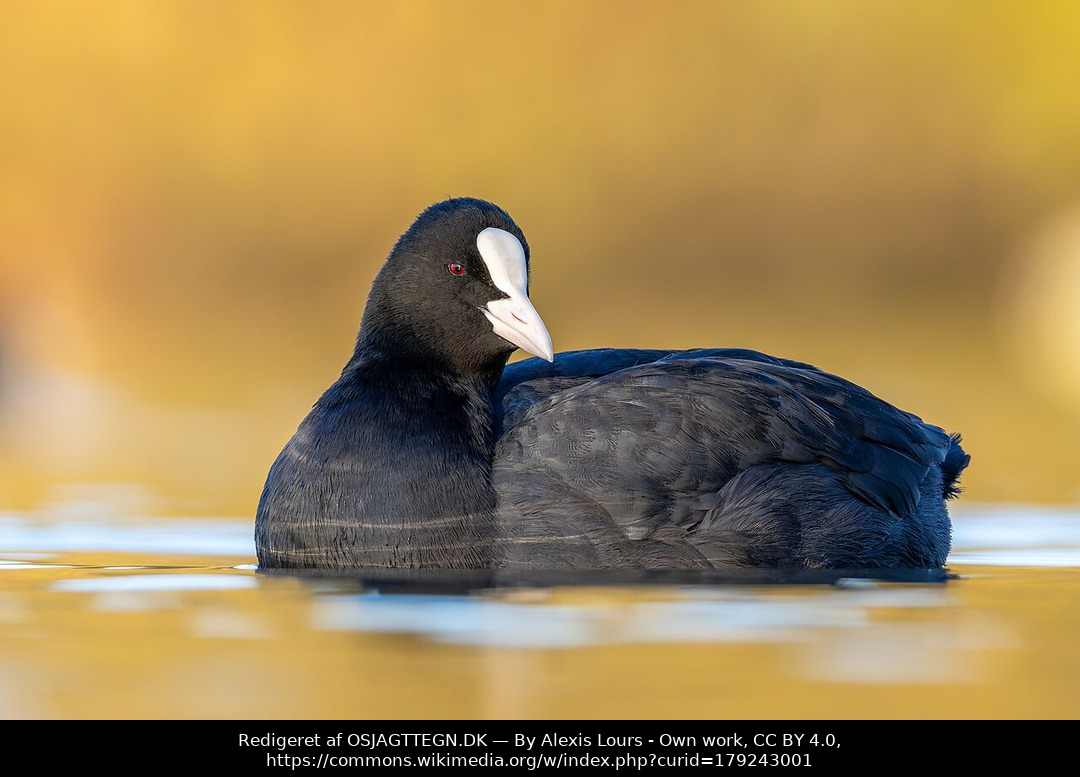
\includegraphics[width=\linewidth, height=7.2cm, keepaspectratio]{Billeder/Dyr/Fugle/Vandhøns/blishoene-01.jpg}
  \end{columns}
\end{frame}
% ========== GRØNBENET RØRHØNE ==========
\begin{frame}{%
  \begin{minipage}[c]{0.30\textwidth}
    Grønbenet rørhøne
  \end{minipage}%
  \hfill
  \begin{minipage}[c]{0.45\textwidth}
    \footnotesize
    \textbf{Jagttid:} Ingen jagttid
  \end{minipage}%
  \hfill
  \begin{minipage}[c]{0.15\textwidth}
    \noindent\raggedleft
    
\includegraphics[width=0.5cm, height=0.5cm, keepaspectratio]{Billeder/Ikoner/star.png}
  \end{minipage}%
}
  \vspace{0.25em}
  \begin{columns}[T]
    \column{0.45\textwidth}
    \setlength{\parskip}{0.5em}
    \tiny
    \RaggedRight
    \textbf{\textit{Gallinula chloropus}} – slankere end blishønen \par
    \textbf{Udseende:}\\
    \quad – Sort med hvid flankestribe \\
    \quad – Rødt næb med gul spids \\
    \quad – Rødt pandeskjold og grønlige ben
    \column{0.52\textwidth}
    \centering
    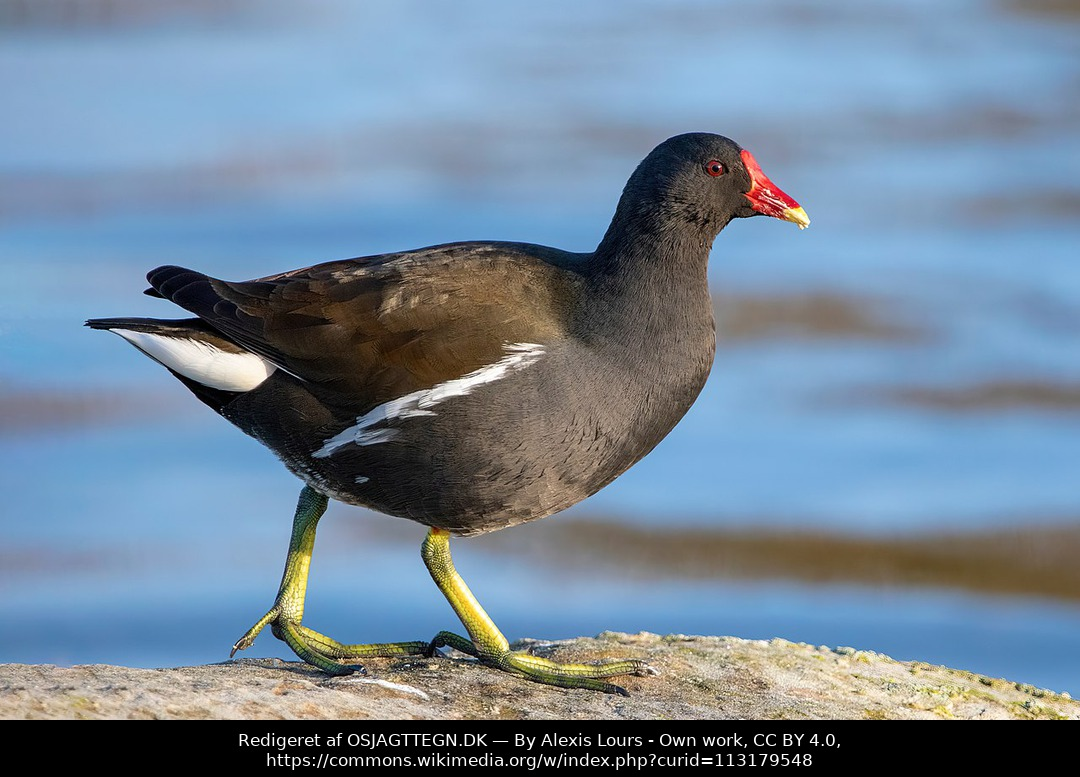
\includegraphics[width=\linewidth, height=7.2cm, keepaspectratio]{Billeder/Dyr/Fugle/Vandhøns/groenbenetroerhoene-02.jpg}
  \end{columns}
\end{frame}
\begin{frame}
  \vspace{1.8em}
  \begin{center}
    \begin{minipage}{0.22\textwidth}
      \centering
      
\includegraphics[width=\linewidth]{Billeder/Dyr/Fugle/Vandhøns/qr/vandhøns_qr.png}
    \end{minipage}%
    \hspace{0.8em}%
    \begin{minipage}{0.62\textwidth}
      \raggedright
      \Large
      \textbf{Træning i artsbestemmelse af vandhøns}\\[0.35em]
      {\large https://osjagttegn.dk/vandhoens}
    \end{minipage}
  \end{center}
\end{frame}
% ========== TITEL: SPURVEFUGLE ==========
\begin{frame}
  \vspace{1.5em}
  \begin{center}
    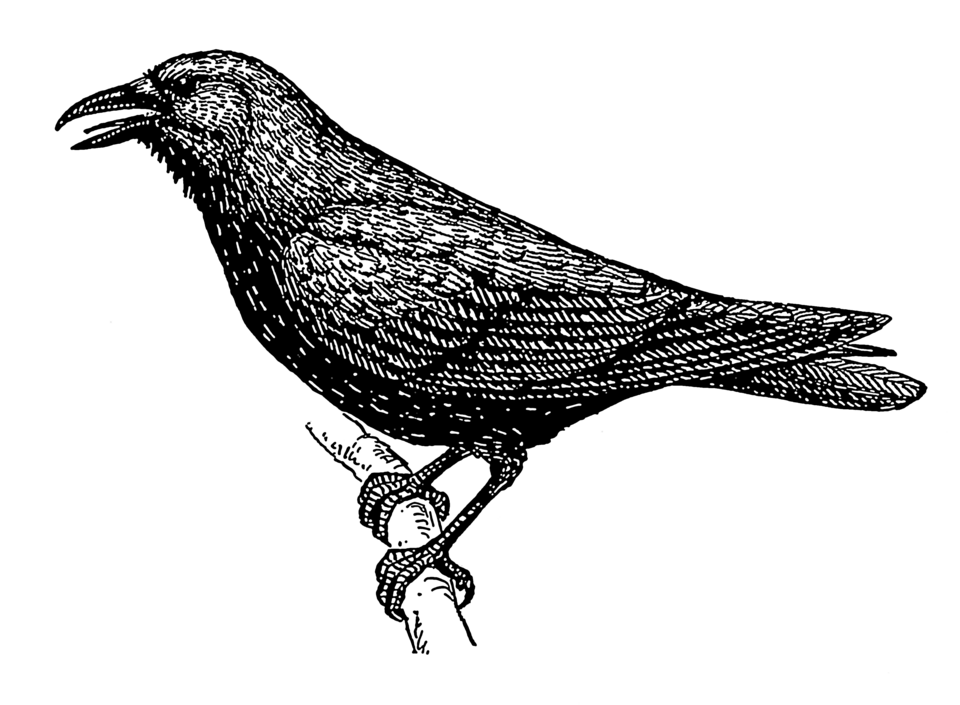
\includegraphics[width=12cm, height=4cm, keepaspectratio]{Billeder/Dyr/Fugle/Spurvefugle/spurvefugle.png}\\[1.2em]
    {\LARGE \textbf{Spurvefugle}}\\[0.6em]
    Artsbestemmelse \& vildtbiologi \\[0.9em]
    {\tiny\color{gray}
    CC BY 4.0 – kan frit anvendes, også kommercielt. Rettighederne må ikke skærpes.\\[0.05em]
    Udviklet af Aleksander Sønder, OSJAGTTEGN.DK}
  \end{center}
\end{frame}

\section{Spurvefugle/Kragefugle (vildtkending og biologi)}

% ========== SORTKRAGE ==========
\begin{frame}{%
  \begin{minipage}[c]{0.30\textwidth}
    Sortkrage (Krage)
  \end{minipage}%
  \hfill
  \begin{minipage}[c]{0.45\textwidth}
    \footnotesize
    \textbf{Jagttid:} 1.\ september -- 31.\ januar
  \end{minipage}%
  \hfill
  \begin{minipage}[c]{0.15\textwidth}
    \noindent\raggedleft
    
\includegraphics[width=0.5cm, height=0.5cm, keepaspectratio]{Billeder/Ikoner/star.png}%
    \hspace{0.2em}%
    
\includegraphics[width=0.5cm, height=0.5cm, keepaspectratio]{Billeder/Ikoner/star.png}%
    \hspace{0.2em}%
    
\includegraphics[width=0.5cm, height=0.5cm, keepaspectratio]{Billeder/Ikoner/star.png}
  \end{minipage}%
}
  \vspace{0.25em}
  \begin{columns}[T]
    \column{0.45\textwidth}
    \setlength{\parskip}{0.45em}
    \tiny
    \RaggedRight
    \textbf{\textit{Corvus corone}} – mellemstor kragefugl, nært beslægtet med gråkrage \par
    \textbf{Udseende:}\\
    \quad – Heltsort krop og hoved \\
    \quad – Sorte øjne \\
    \quad – Ligner ravn, men er mindre og har slankere næb \par
    \textbf{Levesteder:} Alle landskabstyper. \par
    \textbf{Føde:} Opportunist – spiser alt, inkl.\ yngel. \par
    \textbf{Udbredelse:} Især Vestjylland. Sjældnere i resten af landet. \par
    \textbf{Træk/standfugl:} Begge \par
    \textbf{Forplantning:}\\
    \quad – \textbf{Yngleforhold:} Yngler i høje træer. Parret forsvarer territoriet \\
    \quad – \textbf{Kønsmoden:} 2 år \\
    \quad – \textbf{Mono/polygam:} Monogam \\
    \quad – \textbf{Bestandsomsætning:} Langsom \\
    \quad – \textbf{Kuld:} 4--6 æg
    \column{0.52\textwidth}
    \centering
    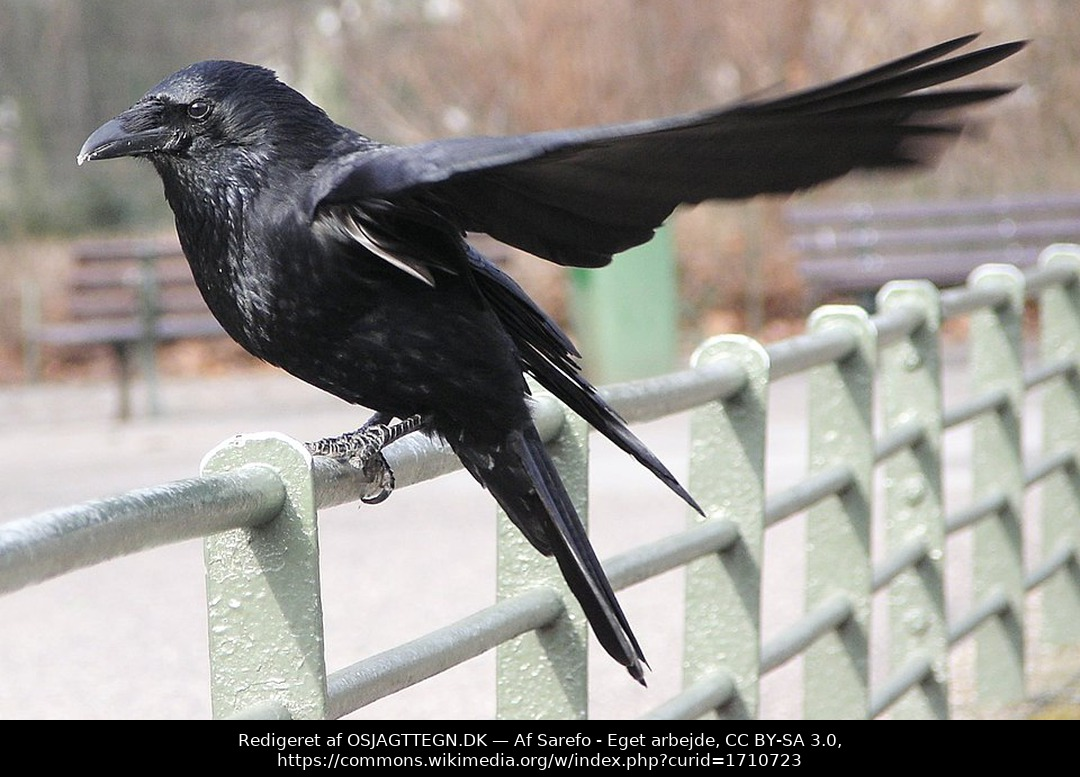
\includegraphics[width=\linewidth, height=7.2cm, keepaspectratio]{Billeder/Dyr/Fugle/Spurvefugle/sortkrage-01.jpg}
  \end{columns}
\end{frame}
% ========== GRÅKRAGE ==========
\begin{frame}{%
  \begin{minipage}[c]{0.30\textwidth}
    Gråkrage (Krage)
  \end{minipage}%
  \hfill
  \begin{minipage}[c]{0.45\textwidth}
    \footnotesize
    \textbf{Jagttid:} 1.\ september -- 31.\ januar
  \end{minipage}%
  \hfill
  \begin{minipage}[c]{0.15\textwidth}
    \noindent\raggedleft
    
\includegraphics[width=0.5cm, height=0.5cm, keepaspectratio]{Billeder/Ikoner/star.png}%
    \hspace{0.2em}%
    
\includegraphics[width=0.5cm, height=0.5cm, keepaspectratio]{Billeder/Ikoner/star.png}%
    \hspace{0.2em}%
    
\includegraphics[width=0.5cm, height=0.5cm, keepaspectratio]{Billeder/Ikoner/star.png}
  \end{minipage}%
}
  \vspace{0.25em}
  \begin{columns}[T]
    \column{0.45\textwidth}
    \setlength{\parskip}{0.45em}
    \tiny
    \RaggedRight
    \textbf{\textit{Corvus cornix}} – mellemstor kragefugl, den almindeligste krage i Danmark \par
    \textbf{Udseende:}\\
    \quad – Grå krop \\
    \quad – Sort hoved, bryst og vinger \\
    \quad – Sorte øjne \par
    \textbf{Levesteder:} Alle landskabstyper. \par
    \textbf{Føde:} Opportunist – spiser alt, inkl.\ yngel. \par
    \textbf{Udbredelse:} Hele Danmark. \par
    \textbf{Træk/standfugl:} Begge \par
    \textbf{Forplantning:}\\
    \quad – \textbf{Yngleforhold:} Yngler i høje træer. Parret forsvarer territoriet \\
    \quad – \textbf{Kønsmoden:} 2 år \\
    \quad – \textbf{Mono/polygam:} Monogam \\
    \quad – \textbf{Bestandsomsætning:} Langsom \\
    \quad – \textbf{Kuld:} 4--6 æg
    \column{0.52\textwidth}
    \centering
    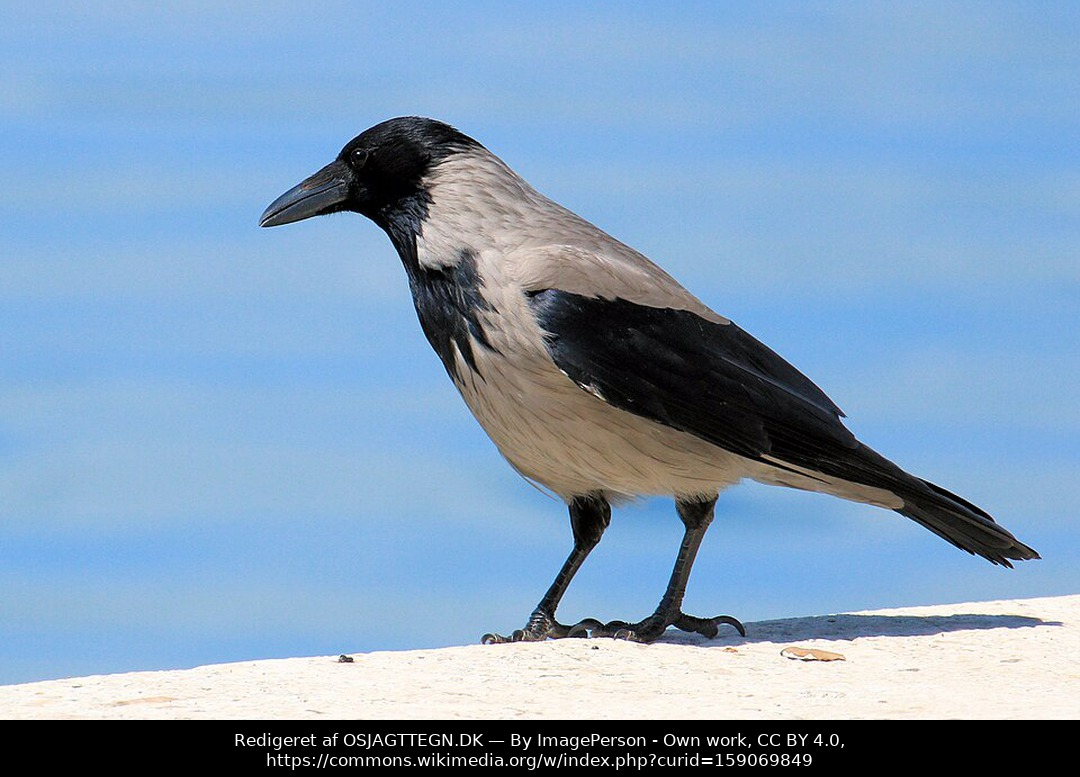
\includegraphics[width=\linewidth, height=7.2cm, keepaspectratio]{Billeder/Dyr/Fugle/Spurvefugle/graakrage-02.jpg}
  \end{columns}
\end{frame}

% ========== RAVN ==========
\begin{frame}{%
  \begin{minipage}[c]{0.30\textwidth}
    Ravn
  \end{minipage}%
  \hfill
  \begin{minipage}[c]{0.45\textwidth}
    \footnotesize
    \textbf{Jagttid:} Ingen jagttid
  \end{minipage}%
  \hfill
  \begin{minipage}[c]{0.15\textwidth}
    \noindent\raggedleft
    
\includegraphics[width=0.5cm, height=0.5cm, keepaspectratio]{Billeder/Ikoner/star.png}
  \end{minipage}%
}
  \vspace{0.25em}
  \begin{columns}[T]
    \column{0.45\textwidth}
    \setlength{\parskip}{0.5em}
    \tiny
    \RaggedRight
    \textbf{\textit{Corvus corax}} – stor, sort kragefugl med kraftigt næb \par
    \textbf{Udseende:}\\
    \quad – Heltsort fjerdragt \\
    \quad – Små fjer går ud på næbbet \\
    \quad – Kraftigere bygget end de øvrige kragefugle
    \column{0.52\textwidth}
    \centering
    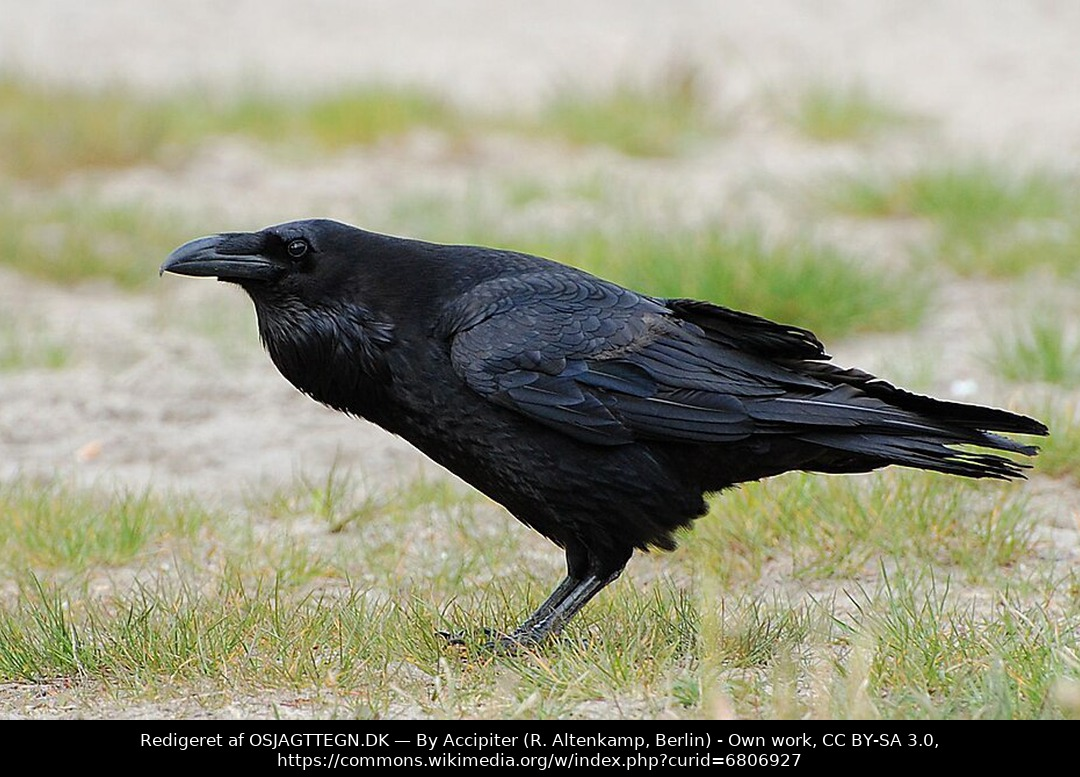
\includegraphics[width=\linewidth, height=7.2cm, keepaspectratio]{Billeder/Dyr/Fugle/Spurvefugle/ravn-01.jpg}
  \end{columns}
\end{frame}
% ========== RÅGE ==========
\begin{frame}{%
  \begin{minipage}[c]{0.30\textwidth}
    Råge
  \end{minipage}%
  \hfill
  \begin{minipage}[c]{0.45\textwidth}
    \footnotesize
    \textbf{Jagttid:} Ingen jagttid
  \end{minipage}%
  \hfill
  \begin{minipage}[c]{0.15\textwidth}
    \noindent\raggedleft
    
\includegraphics[width=0.5cm, height=0.5cm, keepaspectratio]{Billeder/Ikoner/star.png}%
    \hspace{0.2em}%
    
\includegraphics[width=0.5cm, height=0.5cm, keepaspectratio]{Billeder/Ikoner/star.png}
  \end{minipage}%
}
  \vspace{0.25em}
  \begin{columns}[T]
    \column{0.45\textwidth}
    \setlength{\parskip}{0.5em}
    \tiny
    \RaggedRight
    \textbf{\textit{Corvus frugilegus}} – kolonirugende kragefugl med fjerløs næbrod \par
    \textbf{Udseende:}\\
    \quad – Sort med metallisk skær \\
    \quad – Bart, gult eller gråligt parti ved næbbets rod \par
    \textbf{Levesteder:} Alle landskabstyper, men hyppigere ved byer. \par
    \textbf{Føde:} Plantemateriale suppleret med insekter og lignende. \par
    \textbf{Udbredelse:} Hele Danmark. \par
    \textbf{Træk/standfugl:} Standfugl
    \column{0.52\textwidth}
    \centering
    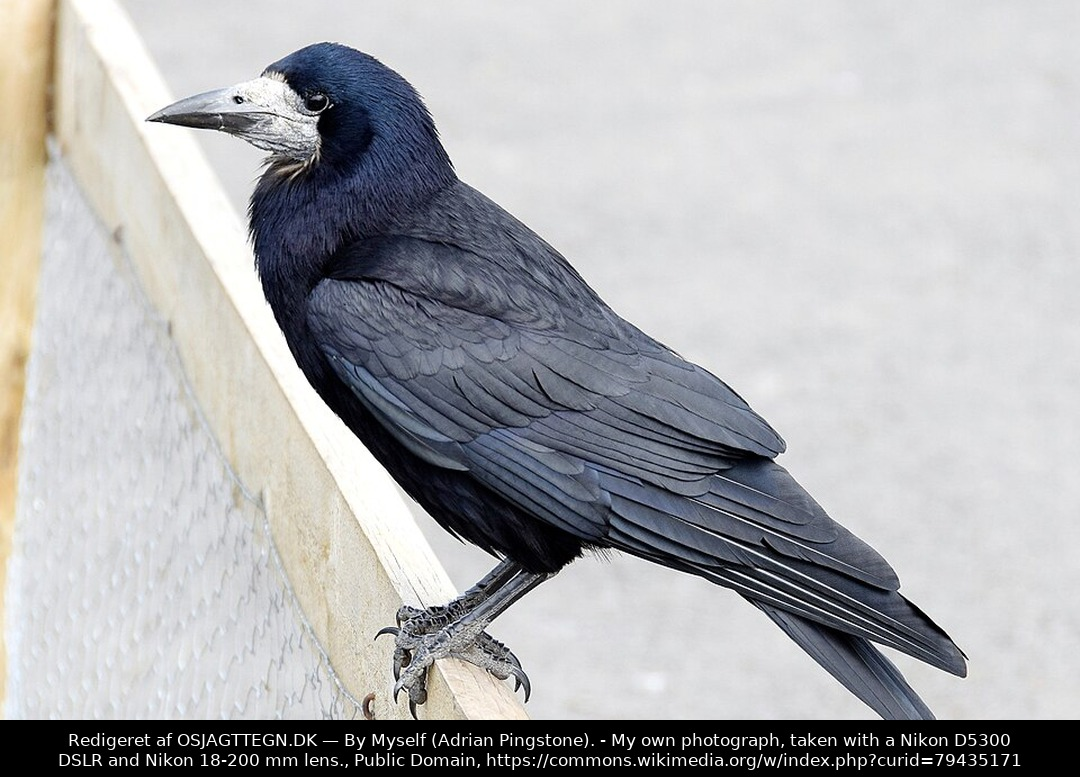
\includegraphics[width=\linewidth, height=7.2cm, keepaspectratio]{Billeder/Dyr/Fugle/Spurvefugle/raage-01.jpg}
  \end{columns}
\end{frame}
% ========== ALLIKE ==========
\begin{frame}{%
  \begin{minipage}[c]{0.30\textwidth}
    Allike
  \end{minipage}%
  \hfill
  \begin{minipage}[c]{0.45\textwidth}
    \footnotesize
    \textbf{Jagttid:} Ingen jagttid
  \end{minipage}%
  \hfill
  \begin{minipage}[c]{0.15\textwidth}
    \noindent\raggedleft
    
\includegraphics[width=0.5cm, height=0.5cm, keepaspectratio]{Billeder/Ikoner/star.png}
  \end{minipage}%
}
  \vspace{0.25em}
  \begin{columns}[T]
    \column{0.45\textwidth}
    \setlength{\parskip}{0.5em}
    \tiny
    \RaggedRight
    \textbf{\textit{Coloeus monedula}} – mindste kragefugl i Danmark med hvidgule øjne \par
    \textbf{Udseende:}\\
    \quad – Mindre end de andre kragefugle \\
    \quad – Grå nakke og hals \\
    \quad – Kendes især på det hvidgule øje
    \column{0.52\textwidth}
    \centering
    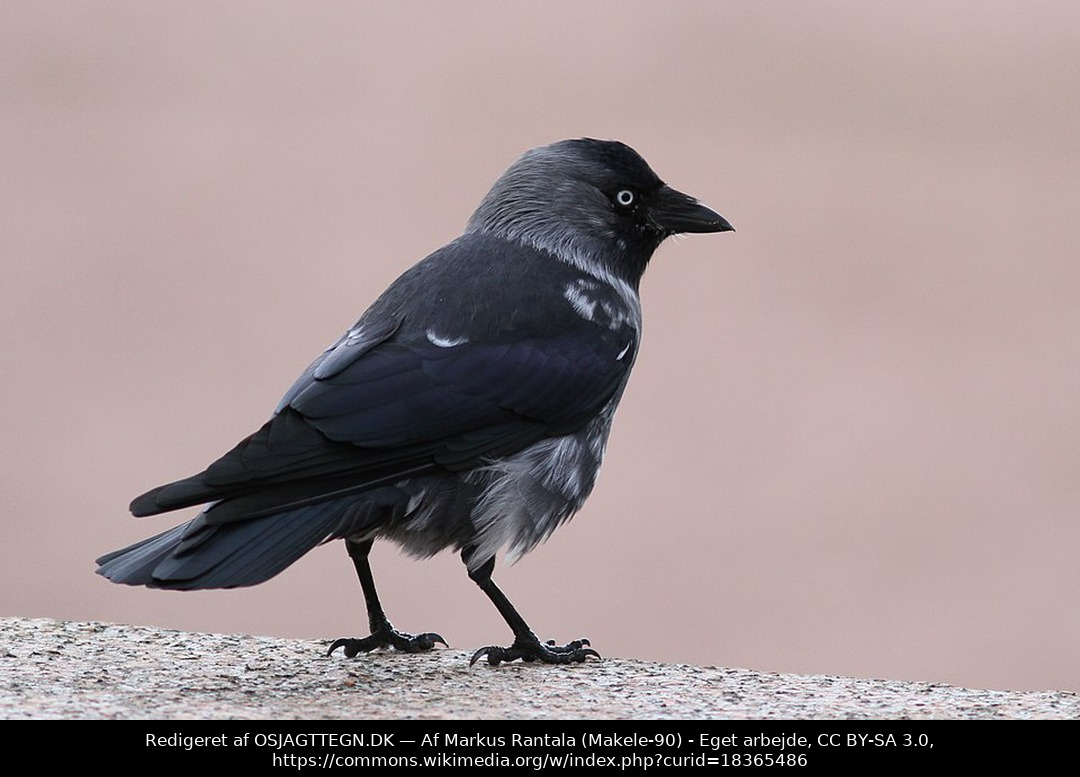
\includegraphics[width=\linewidth, height=7.2cm, keepaspectratio]{Billeder/Dyr/Fugle/Spurvefugle/allike-01.jpg}
  \end{columns}
\end{frame}
% ========== HUSSKADE ==========
\begin{frame}{%
  \begin{minipage}[c]{0.30\textwidth}
    Husskade
  \end{minipage}%
  \hfill
  \begin{minipage}[c]{0.45\textwidth}
    \footnotesize
    \textbf{Jagttid:} 1.\ september -- 31.\ januar
  \end{minipage}%
  \hfill
  \begin{minipage}[c]{0.15\textwidth}
    \noindent\raggedleft
    
\includegraphics[width=0.5cm, height=0.5cm, keepaspectratio]{Billeder/Ikoner/star.png}%
    \hspace{0.2em}%
    
\includegraphics[width=0.5cm, height=0.5cm, keepaspectratio]{Billeder/Ikoner/star.png}
  \end{minipage}%
}
  \vspace{0.25em}
  \begin{columns}[T]
    \column{0.45\textwidth}
    \setlength{\parskip}{0.5em}
    \tiny
    \RaggedRight
    \textbf{\textit{Pica pica}} – kendes på den lange hale og den sort-hvide fjerdragt \par
    \textbf{Udseende:}\\
    \quad – Sort og hvid med blågrønne metalskær \\
    \quad – Hoved og ryg sorte \\
    \quad – Bug og dele af vingerne hvide \par
    \textbf{Levesteder:} Alle landskabstyper, oftest i bynære zoner. \par
    \textbf{Føde:} Altædende. \par
    \textbf{Udbredelse:} Hele Danmark. \par
    \textbf{Træk/standfugl:} Standfugl
    \column{0.52\textwidth}
    \centering
    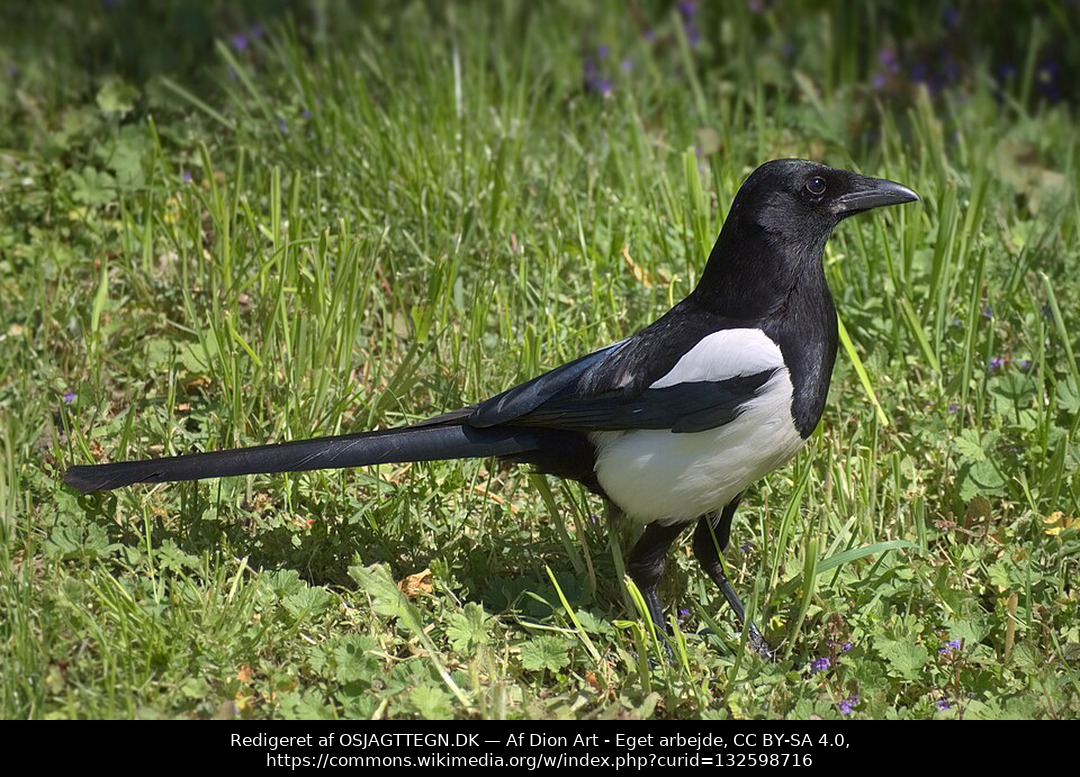
\includegraphics[width=\linewidth, height=7.2cm, keepaspectratio]{Billeder/Dyr/Fugle/Spurvefugle/husskade-01.jpg}
  \end{columns}
\end{frame}
% ========== SKOVSKADE ==========
\begin{frame}{%
  \begin{minipage}[c]{0.30\textwidth}
    Skovskade
  \end{minipage}%
  \hfill
  \begin{minipage}[c]{0.45\textwidth}
    \footnotesize
    \textbf{Jagttid:} Ingen jagttid
  \end{minipage}%
  \hfill
  \begin{minipage}[c]{0.15\textwidth}
    \noindent\raggedleft
    
\includegraphics[width=0.5cm, height=0.5cm, keepaspectratio]{Billeder/Ikoner/star.png}
  \end{minipage}%
}
  \vspace{0.25em}
  \begin{columns}[T]
    \column{0.45\textwidth}
    \setlength{\parskip}{0.5em}
    \tiny
    \RaggedRight
    \textbf{\textit{Garrulus glandarius}} – kendes på den rødbrune fjerdragt og det lyseblå felt på vingen \par
    \textbf{Udseende:}\\
    \quad – Rødbrun med hvid strube \\
    \quad – Sort hale \\
    \quad – Lyseblåt felt med sorte striber på vingen
    \column{0.52\textwidth}
    \centering
    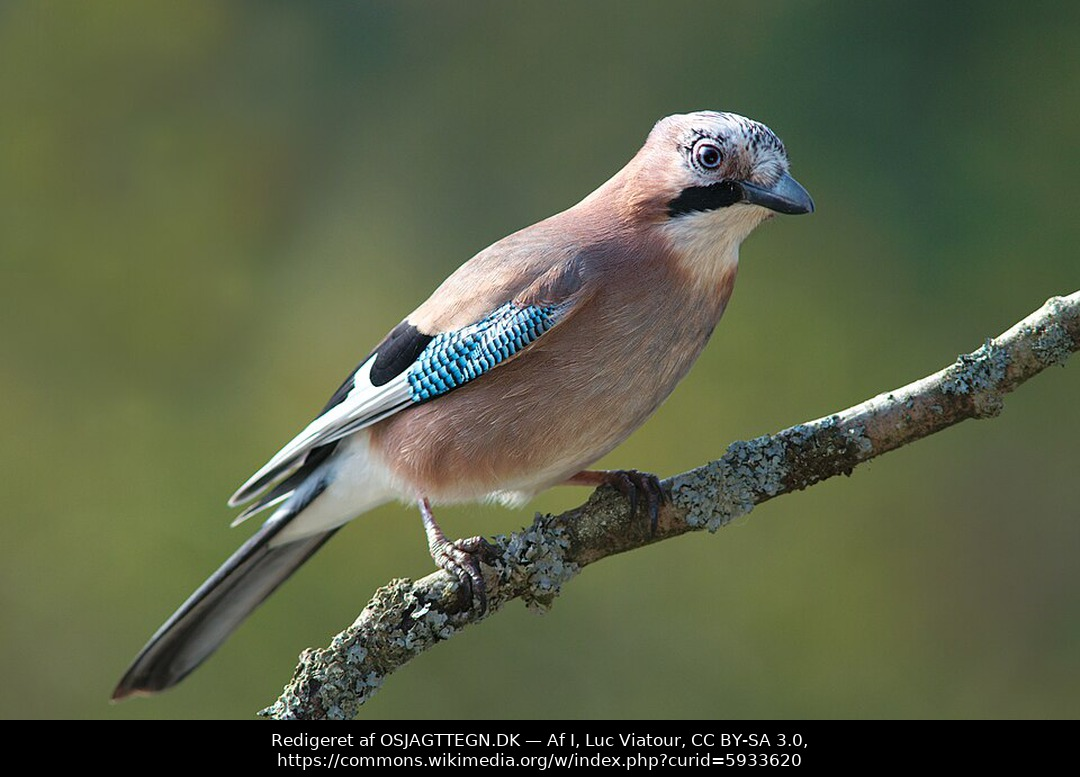
\includegraphics[width=\linewidth, height=7.2cm, keepaspectratio]{Billeder/Dyr/Fugle/Spurvefugle/skovskade-01.jpg}
  \end{columns}
\end{frame}

\begin{frame}
  \vspace{1.8em}
  \begin{center}
    \begin{minipage}{0.22\textwidth}
      \centering
      
\includegraphics[width=\linewidth]{Billeder/Dyr/Fugle/Spurvefugle/qr/spurvefugle_qr.png}
    \end{minipage}%
    \hspace{0.8em}%
    \begin{minipage}{0.62\textwidth}
      \raggedright
      \Large
      \textbf{Træning i artsbestemmelse af spurvefugle}\\[0.35em]
      {\large https://osjagttegn.dk/spurvefugle}
    \end{minipage}
  \end{center}
\end{frame}
% ========== TITEL: DUER ==========
\begin{frame}
  \vspace{1.5em}
  \begin{center}
    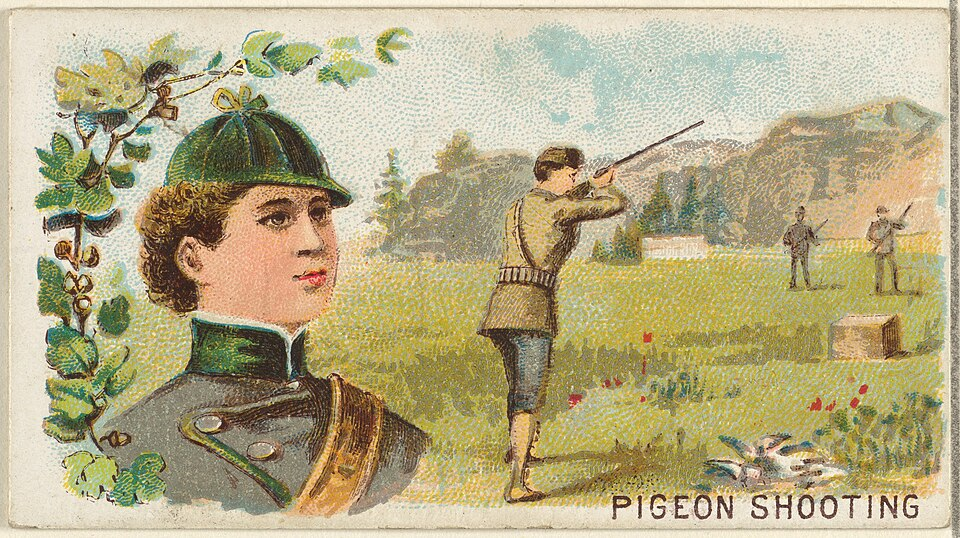
\includegraphics[width=12cm, height=4cm, keepaspectratio]{Billeder/Dyr/Fugle/Duer/duer.jpg}\\[1.2em]
    {\LARGE \textbf{Duer}}\\[0.6em]
    Artsbestemmelse \& vildtbiologi \\[0.9em]
    {\tiny\color{gray}
    CC BY 4.0 – kan frit anvendes, også kommercielt. Rettighederne må ikke skærpes.\\[0.05em]
    Udviklet af Aleksander Sønder, OSJAGTTEGN.DK}
  \end{center}
\end{frame}

\section{Duer (vildtkending og biologi)}

% ========== RINGDUE ==========
\begin{frame}{%
  \begin{minipage}[c]{0.30\textwidth}
    Ringdue
  \end{minipage}%
  \hfill
  \begin{minipage}[c]{0.45\textwidth}
    \footnotesize
    \textbf{Jagttid:} 11.\ november -- 31.\ januar
  \end{minipage}%
  \hfill
  \begin{minipage}[c]{0.15\textwidth}
    \noindent\raggedleft
    
\includegraphics[width=0.5cm, height=0.5cm, keepaspectratio]{Billeder/Ikoner/star.png}%
    \hspace{0.2em}%
    
\includegraphics[width=0.5cm, height=0.5cm, keepaspectratio]{Billeder/Ikoner/star.png}%
    \hspace{0.2em}%
    
\includegraphics[width=0.5cm, height=0.5cm, keepaspectratio]{Billeder/Ikoner/star.png}
  \end{minipage}%
}
  \vspace{0.25em}
  \begin{columns}[T]
    \column{0.45\textwidth}
    \setlength{\parskip}{0.45em}
    \tiny
    \RaggedRight
    \textbf{\textit{Columba palumbus}} – mest almindelige due i Danmark, også kaldet skovdue \par
    \textbf{Udseende:}\\
    \quad – Gråblå fjerdragt \\
    \quad – Hvid halsplet \\
    \quad – Gult næb \par
    \textbf{Levesteder:} Alle landskabstyper, hyppigst nær byer. \par
    \textbf{Føde:} Plantefrø og landbrugsafgrøder. \par
    \textbf{Udbredelse:} Hele Danmark. \par
    \textbf{Træk/standfugl:} Begge \par
    \textbf{Forplantning:}\\
    \quad – \textbf{Yngleforhold:} Bygger enkel rede af kviste \\
    \quad – \textbf{Kønsmoden:} 1 år \\
    \quad – \textbf{Mono/polygam:} Monogam \\
    \quad – \textbf{Bestandsomsætning:} Hurtig \\
    \quad – \textbf{Kuld:} 2 æg, 2--4 gange om året
    \column{0.52\textwidth}
    \centering
    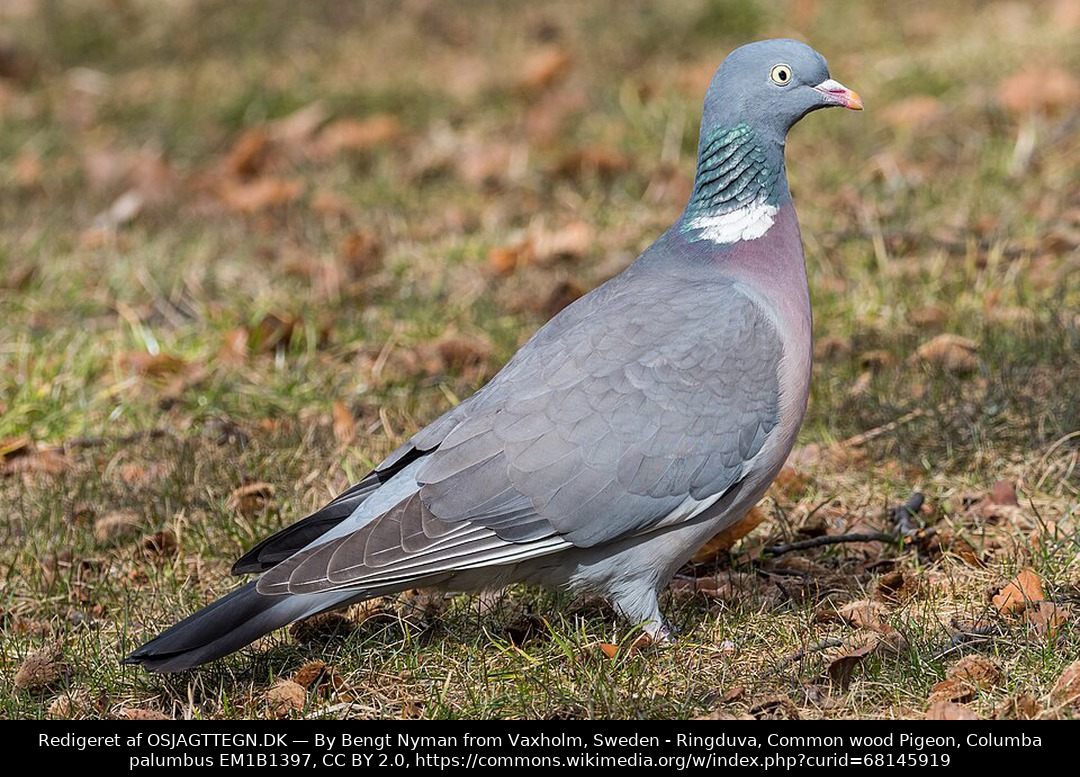
\includegraphics[width=\linewidth, height=7.2cm, keepaspectratio]{Billeder/Dyr/Fugle/Duer/ringdue-01.jpg}
  \end{columns}
\end{frame}
% ========== TYRKERDUE ==========
\begin{frame}{%
  \begin{minipage}[c]{0.30\textwidth}
    Tyrkerdue
  \end{minipage}%
  \hfill
  \begin{minipage}[c]{0.45\textwidth}
    \footnotesize
    \textbf{Jagttid:} Ingen jagttid
  \end{minipage}%
  \hfill
  \begin{minipage}[c]{0.15\textwidth}
    \noindent\raggedleft
    
\includegraphics[width=0.5cm, height=0.5cm, keepaspectratio]{Billeder/Ikoner/star.png}
  \end{minipage}%
}
  \vspace{0.25em}
  \begin{columns}[T]
    \column{0.45\textwidth}
    \setlength{\parskip}{0.5em}
    \tiny
    \RaggedRight
    \textbf{\textit{Streptopelia decaocto}} – lille, slank due \par
    \textbf{Udseende:}\\
    \quad – Lyst beigegrå eller sandfarvet \\
    \quad – Lang hale og forholdsvis smalle vinger med afrundede, mørke vingespidser \\
    \quad – Tydeligt sort, halvcirkelformet nakkebånd
    \column{0.52\textwidth}
    \centering
    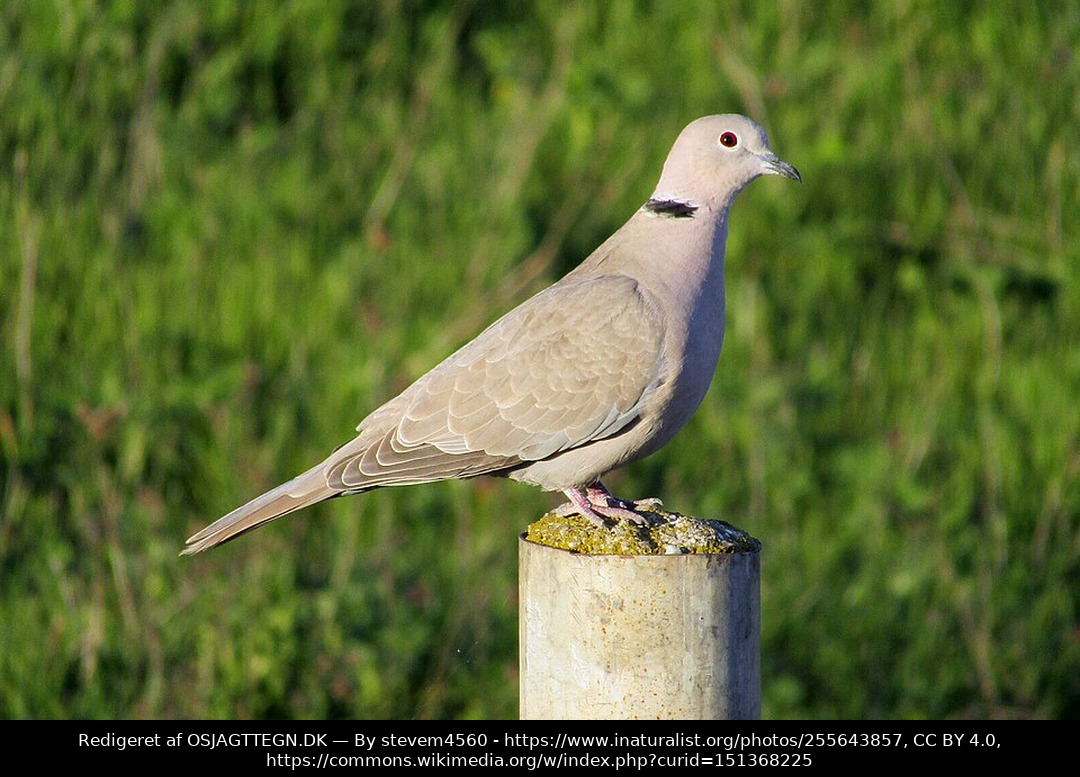
\includegraphics[width=\linewidth, height=7.2cm, keepaspectratio]{Billeder/Dyr/Fugle/Duer/tyrkerdue-01.jpg}
  \end{columns}
\end{frame}
% ========== HULDUE ==========
\begin{frame}{%
  \begin{minipage}[c]{0.30\textwidth}
    Huldue
  \end{minipage}%
  \hfill
  \begin{minipage}[c]{0.45\textwidth}
    \footnotesize
    \textbf{Jagttid:} Ingen jagttid
  \end{minipage}%
  \hfill
  \begin{minipage}[c]{0.15\textwidth}
    \noindent\raggedleft
    
\includegraphics[width=0.5cm, height=0.5cm, keepaspectratio]{Billeder/Ikoner/star.png}
  \end{minipage}%
}
  \vspace{0.25em}
  \begin{columns}[T]
    \column{0.45\textwidth}
    \setlength{\parskip}{0.5em}
    \tiny
    \RaggedRight
    \textbf{\textit{Columba oenas}} – fåtallig dansk ynglefugl, men temmelig almindelig som trækgæst. Den er fredet. \par
    \textbf{Udseende:}\\
    \quad – Rimelig ensfarvet, blålig fjerdragt \\
    \quad – Grønlig plet på halsen \\
    \quad – To sorte striber på hver vinge
    \column{0.52\textwidth}
    \centering
    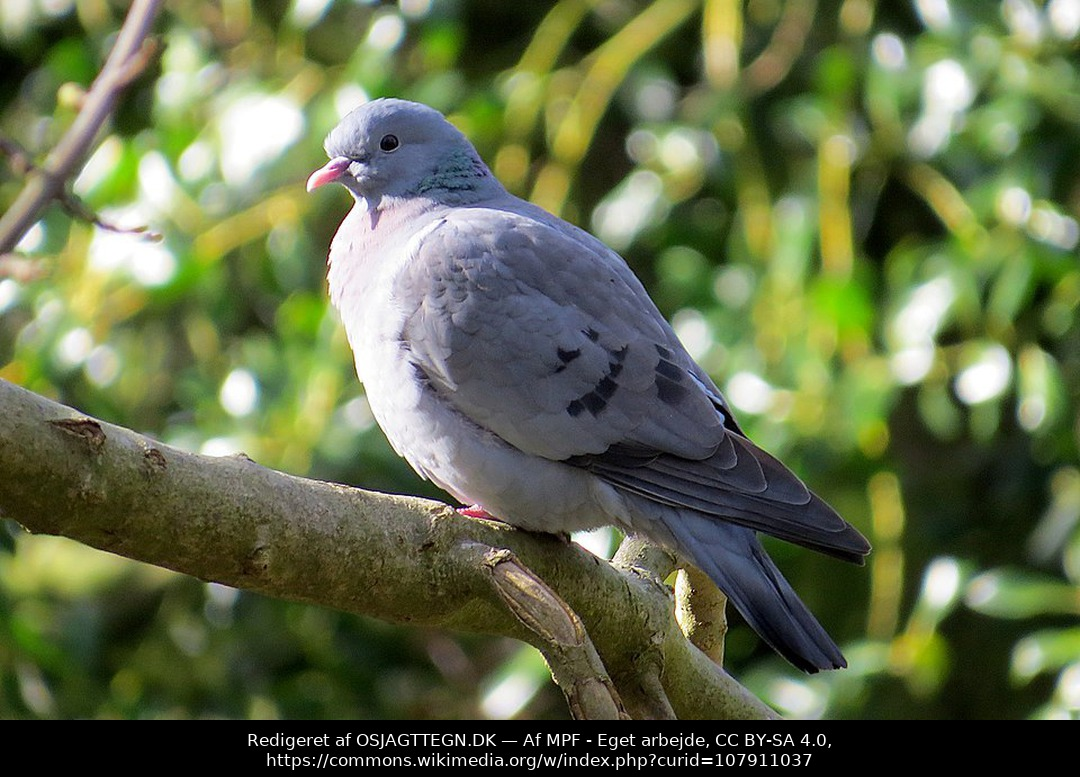
\includegraphics[width=\linewidth, height=7.2cm, keepaspectratio]{Billeder/Dyr/Fugle/Duer/huldue-01.jpg}
  \end{columns}
\end{frame}

\begin{frame}
  \vspace{1.8em}
  \begin{center}
    \begin{minipage}{0.22\textwidth}
      \centering
      
\includegraphics[width=\linewidth]{Billeder/Dyr/Fugle/Duer/duer_qr.png}
    \end{minipage}%
    \hspace{0.8em}%
    \begin{minipage}{0.62\textwidth}
      \raggedright
      \Large
      \textbf{Træning i artsbestemmelse af duer}\\[0.35em]
      {\large https://osjagttegn.dk/duer}
    \end{minipage}
  \end{center}
\end{frame}

\section{Jagttermer Del 2}

\begin{frame}
  \vspace{3em}
  \begin{center}
    {\LARGE \textbf{Jagttermer - Del 2}
    }
    \\
    \vspace{1em}
  \end{center}
\end{frame}


\begin{frame}{Jagttermer - Del 2 (H-P)}

\vspace{0.3em} % Mindre top-afstand

\begin{columns}[T]
    % --- Venstre kolonne: H, J, K ---
    \column{0.48\textwidth}
    \textbf{\large H, J, K}
    \setlength{\parskip}{0.1em} % Mindre afstand mellem punkter
    \scriptsize % Mindre skriftstørrelse
    \RaggedRight
    \begin{itemize}
        \item \textbf{Jagtkonsortium:} Gruppe af personer, der har lejet et jagtareal sammen.
        \item \textbf{Jagtleder:} Den person, der leder en fællesjagt.
        \item \textbf{Jagttryk:} Den påvirkning, som jagt i form af afskydning og forstyrrelse har på en vildtbestand.
        \item \textbf{Knæk og bræk:} Hilsen som udtrykker ønske om et positivt udbytte for jægere og fiskere. Bruges i stedet for ”Held og lykke”, som ifølge traditionen bringer uheld.
        \item \textbf{Krybskytte:} Person, der driver ulovlig jagt på anden persons jagtområde, på arter uden jagttid eller uden for jagttid på jagtbare arter.
        \item \textbf{Kuglebane:} Riffelprojektilets bane gennem luften på vej mod målet.
        \item \textbf{Kunstgrav:} Menneskabt rævegrav ofte etableret med gravjagt og regulering af ræve for øje.
    \end{itemize}

    % --- Højre kolonne: M, N, O, P ---
    \column{0.48\textwidth}
    \textbf{\large M, N, O, P}
    \setlength{\parskip}{0.1em} % Mindre afstand mellem punkter
    \scriptsize % Mindre skriftstørrelse
    \RaggedRight
    \begin{itemize}
        \item \textbf{Markvildt:} Vildt, der primært lever i det dyrkede agerland. Anvendes især om hare og agerhøne.
        \item \textbf{Nedlægge:} Skyde og dræbe vildt under jagt.
        \item \textbf{Opsats:} (se beskrivelse under "Gevir")
        \item \textbf{Opbrække:} Rettelig hedder det, brække op: Tage klovbærende vildts indvolde ud.
        \item \textbf{Opfløj:} Jagtudtryk for at fugle letter.
        \item \textbf{Parole:} Jagtlederens instruktion til jægerne på en fællesjagt før jagten går i gang.
        \item \textbf{Post:} Tildelt plads på en fællesjagt.
    \end{itemize}
\end{columns}

\end{frame}

\end{document}